\documentclass[11pt,letterpaper]{article}
\usepackage[margin=1in]{geometry}
\usepackage[T1]{fontenc}
\usepackage{lmodern,microtype}
\usepackage{amsmath,amssymb,amsthm,mathtools,bm}
\usepackage{booktabs,array,xcolor,tikz}
\usepackage{flafter}
\usetikzlibrary{arrows.meta,positioning,calc,fit}
\usepackage[colorlinks=true,linkcolor=black,citecolor=black,urlcolor=blue]{hyperref}
\definecolor{navy}{HTML}{20354D}
\definecolor{teal}{HTML}{087E8B}
\definecolor{violet}{HTML}{7656A3}
\definecolor{paleTeal}{HTML}{E5F3F3}
\definecolor{paleViolet}{HTML}{EFEAF6}
\definecolor{amber}{HTML}{B97718}
\definecolor{mist}{HTML}{F3F5F8}
\definecolor{rust}{HTML}{A8432F}
\definecolor{paleRust}{HTML}{F6E3DD}
\definecolor{leaf}{HTML}{3F7D4E}
\definecolor{paleLeaf}{HTML}{E7F1E8}
\newtheorem{theorem}{Theorem}
\newtheorem{lemma}[theorem]{Lemma}
\newtheorem{corollary}[theorem]{Corollary}
\newtheorem{proposition}[theorem]{Proposition}
\theoremstyle{definition}\newtheorem{definition}[theorem]{Definition}
\newtheorem{remark}[theorem]{Remark}
\newcommand{\C}{\mathbb C}
\newcommand{\E}{\mathbb E}
\newcommand{\I}{I}
\newcommand{\Tr}{\operatorname{Tr}}
\newcommand{\TD}{\operatorname{TD}}
\newcommand{\Ad}{\operatorname{Ad}}
\newcommand{\Dom}{\operatorname{Dom}}
\newcommand{\Img}{\operatorname{Im}}
\newcommand{\ket}[1]{\lvert#1\rangle}
\newcommand{\bra}[1]{\langle#1\rvert}
\newcommand{\proj}[1]{\ket{#1}\!\bra{#1}}
\newcommand{\vket}[1]{\lvert#1\rangle\!\rangle}
\newcommand{\vbra}[1]{\langle\!\langle#1\rvert}
\newcommand{\norm}[1]{\lVert#1\rVert}
\newcommand{\SW}{\mathcal S}
\newcommand{\QC}{\mathcal Q}
\newcommand{\id}{\operatorname{id}}
\newcommand{\ind}[1]{\mathbf 1_{\{#1\}}}
\newcommand{\reffig}[1]{Figure~\ref{#1}}
\newcommand{\Same}{\textnormal{\textsc{Same}}}
\newcommand{\Mub}{\textnormal{\textsc{Mub}}}
\newcommand{\before}{\prec}
% Locator of the supplementary material (URL or DOI with commit hash). Fill in before submission,
\makeatletter
\newenvironment{resulttable}{\par\medskip\noindent\begin{minipage}{\textwidth}\def\@captype{table}\centering}{\end{minipage}\par\medskip}
\newenvironment{resultfigure}{\par\medskip\noindent\begin{minipage}{\textwidth}\def\@captype{figure}\centering}{\end{minipage}\par\medskip}
\makeatother
\tikzset{
 flowbox/.style={draw=navy!38,fill=white,rounded corners=3.5pt,line width=.55pt},
 flowend/.style={draw=navy,fill=mist,rounded corners=3.5pt,line width=.9pt},
 flowtab/.style={fill=navy,text=white,font=\small\sffamily\bfseries,rounded corners=2pt,minimum width=.52cm,minimum height=.52cm,inner sep=0pt},
 flowname/.style={font=\small\sffamily\bfseries,text=navy,anchor=west,align=left,inner sep=0pt},
 flownote/.style={font=\small\sffamily,text=navy,anchor=west,align=left,inner sep=0pt},
 flowstep/.style={font=\footnotesize\sffamily\itshape,text=navy!70,anchor=west,inner sep=0pt},
 flowdown/.style={draw=navy!22,line width=5.5pt,-{Triangle[length=6.5pt,width=12.5pt]}},
 fsA/.style={draw=teal,fill=paleTeal,rounded corners=1pt,line width=.6pt,minimum width=.56cm,minimum height=.56cm,font=\small,inner sep=0pt},
 fsB/.style={draw=violet,fill=paleViolet,rounded corners=1pt,line width=.6pt,minimum width=.56cm,minimum height=.56cm,font=\small,inner sep=0pt},
 fsI/.style={draw=navy!35,fill=white,rounded corners=1pt,line width=.5pt,minimum width=.56cm,minimum height=.56cm,font=\scriptsize,text=navy!55,inner sep=0pt},
 figlab/.style={font=\small\sffamily,text=navy,align=center},
 figtitle/.style={font=\small\sffamily\bfseries,text=navy,anchor=west},
 figtiny/.style={font=\scriptsize\sffamily,text=navy,align=center},
 figwire/.style={draw=navy,line width=.7pt},
 figmem/.style={draw=navy,line width=1.6pt},
 gateA/.style={draw=teal,fill=paleTeal,rounded corners=1.5pt,line width=.7pt,minimum width=.78cm,minimum height=.62cm,font=\small,inner sep=1pt},
 gateB/.style={draw=violet,fill=paleViolet,rounded corners=1.5pt,line width=.7pt,minimum width=.78cm,minimum height=.62cm,font=\small,inner sep=1pt},
 gateK/.style={draw=navy,fill=mist,rounded corners=1.5pt,line width=.7pt,minimum width=.62cm,font=\small,inner sep=1pt},
 figcc/.style={draw=amber,line width=.6pt,double,double distance=.9pt,-{Latex[length=4pt,width=4pt]}},
 figpanel/.style={draw=navy!35,fill=mist,rounded corners=4pt,line width=.5pt},
 figstep/.style={font=\small\sffamily\bfseries,text=navy,anchor=north west},
 figarrow/.style={->,draw=navy,line width=1.1pt},
}
\hypersetup{pdftitle={Infinite or indefinite: the query cost of simulating the quantum switch},pdfauthor={Dantong Li}}
\title{Infinite or indefinite:\\ the query cost of simulating the quantum switch}
\author{Dantong Li\\\small Department of Computer Science, Yale University}
\date{November 2026}
\begin{document}
\maketitle

\begin{abstract}
The quantum switch applies two black-box operations in a coherent
superposition of their two orders and calls each of them once. We ask
how many calls an ordinary strategy needs to do the same, where an
ordinary strategy is a quantum circuit that calls the boxes in an order
that is definite on every run and may be chosen adaptively. For unitary
operations three calls suffice. For general quantum channels we prove
three lower bounds. First, for every dimension $d\ge2$, no ordinary strategy
with a bounded number of calls reproduces the switch exactly on all
pairs of channels. Exact simulation therefore requires an indefinite order of
calls or a number of calls that no bound limits. Second, approximate
simulation is expensive: any fixed diamond-norm error below $1/2$
requires $\Omega(d^{1/4})$ calls, which is exponential in the number of
qubits. Third, a single number is already hard. The switch estimates the
interference visibility of its control qubit, which quantifies the
incompatibility of two measurements, with a constant number of uses. An
ordinary strategy needs $\Omega(d^{1/16})$ calls even to decide whether
two measurement devices with hidden bases and unread outcomes perform
the same measurement or maximally incompatible ones, whatever quantum
memory and adaptivity it uses. The same number certifies a mismatch
between a noisy device and a model of its noise. The
three theorems have been formalized in the Lean proof assistant
(Appendix~\ref{sec:formal-status}).
We end by asking in which computational tasks such black boxes arise.
\end{abstract}

\section{Introduction}

In a quantum circuit, operations are applied one after another. Quantum
theory also allows processes in which the order of two operations is
itself a quantum degree of freedom. The simplest is the \emph{quantum
switch}~\cite{chiribella2013}. It takes two black-box operations $A$ and
$B$ and a control qubit. If the control is in the state $\ket0$, a
target system undergoes $A$ and then $B$. If the control is in the state
$\ket1$, the target undergoes $B$ and then $A$. If the control is in a
superposition, so is the order (\reffig{fig:switch}(a)). Each box is called exactly once: the output depends only on the two operations and is linear in each of them. The switch has been realized in several laboratories~\cite{procopio2015,rozema2024}, and it has been reported to help in
discriminating channels~\cite{chiribella2012}, in promise problems on
unknown gates~\cite{araujo2014}, in communication~\cite{guerin2016,ebler2018}, in
metrology~\cite{zhao2020}, and in measuring the incompatibility of quantum measurements~\cite{gao2023}. Some of these advantages have since been reassessed against other resources, such as coherent control of the channels~\cite{abbott2020} and more general strategies with a definite order~\cite{mothe2024}.

\begin{figure}[t]
\centering
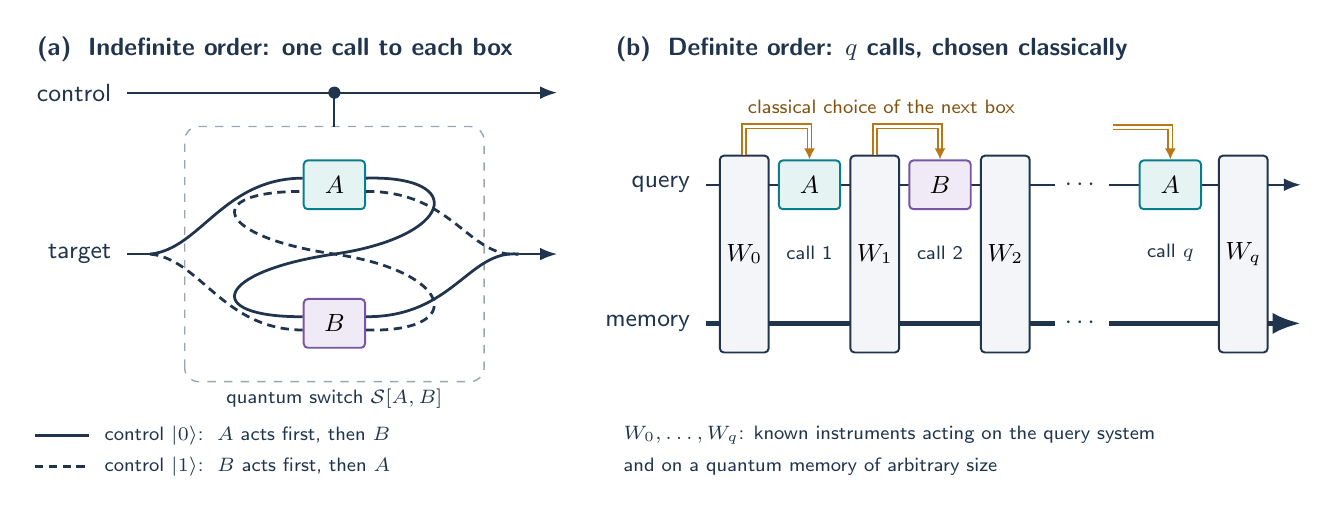
\begin{tikzpicture}[x=.975cm,y=1cm,>=Latex]
%% ---------- panel (a): the switch ----------
\node[figtitle] at (-1.3,2.6) {(a)\; Indefinite order: one call to each box};
\draw[draw=navy!45,dashed,rounded corners=5pt,line width=.5pt] (.75,-1.62) rectangle (4.65,1.62);
\node[figtiny] at (2.7,-1.84) {quantum switch $\SW[A,B]$};
\node[gateA] (A) at (2.7,.88) {$A$};
\node[gateB] (B) at (2.7,-.88) {$B$};
% control |0>: A then B (teal, solid)
\draw[draw=navy,line width=1pt] (.3,.0) .. controls (.95,.06) and (1.25,.96) .. ([yshift=2.4pt]A.west);
\draw[draw=navy,line width=1pt] ([yshift=2.4pt]A.east) .. controls (4.45,1.0) and (4.25,.22) .. (2.7,.0)
      .. controls (1.15,-.22) and (.95,-.80) .. ([yshift=2.4pt]B.west);
\draw[draw=navy,line width=1pt] ([yshift=2.4pt]B.east) .. controls (4.25,-.80) and (4.45,.06) .. (5.1,.0);
% control |1>: B then A (violet, dashed)
\draw[draw=navy,line width=1pt,densely dashed] (.3,.0) .. controls (.95,-.06) and (1.25,-.96) .. ([yshift=-2.4pt]B.west);
\draw[draw=navy,line width=1pt,densely dashed] ([yshift=-2.4pt]B.east) .. controls (4.45,-1.0) and (4.25,-.22) .. (2.7,.0)
      .. controls (1.15,.22) and (.95,.80) .. ([yshift=-2.4pt]A.west);
\draw[draw=navy,line width=1pt,densely dashed] ([yshift=-2.4pt]A.east) .. controls (4.25,.80) and (4.45,-.06) .. (5.1,.0);
\draw[figwire] (0,0) -- (.3,0); \draw[figwire,->] (5.1,0) -- (5.6,0);
% control wire
\draw[figwire,->] (0,2.05) -- (5.6,2.05);
\fill[navy] (2.7,2.05) circle (2.2pt);
\draw[figwire] (2.7,2.05) -- (2.7,1.62);
\node[figlab,anchor=east] at (-.08,2.05) {control};
\node[figlab,anchor=east] at (-.08,0) {target};
% legend, stacked
\draw[draw=navy,line width=1pt] (-1.2,-2.3) -- (-.5,-2.3);
\node[figtiny,anchor=west] at (-.42,-2.3) {control $\ket0$:\ \ $A$ acts first, then $B$};
\draw[draw=navy,line width=1pt,densely dashed] (-1.2,-2.7) -- (-.5,-2.7);
\node[figtiny,anchor=west] at (-.42,-2.7) {control $\ket1$:\ \ $B$ acts first, then $A$};
%% ---------- panel (b): an ordinary strategy ----------
\begin{scope}[xshift=7.35cm]
\node[figtitle] at (-1.3,2.6) {(b)\; Definite order: $q$ calls, chosen classically};
\draw[figwire] (0,.88) -- (4.55,.88);  \draw[figwire,->] (5.25,.88) -- (7.75,.88);
\draw[figmem] (0,-.88) -- (4.55,-.88); \draw[figmem,->] (5.25,-.88) -- (7.75,-.88);
\node[figlab] at (4.9,.88) {$\cdots$}; \node[figlab] at (4.9,-.88) {$\cdots$};
\foreach \x/\l in {.5/0,2.2/1,3.9/2,7.0/q}
  \node[gateK,minimum height=2.5cm] (W\l) at (\x,0) {$W_{\l}$};
\node[gateA] (s1) at (1.35,.88) {$A$};
\node[gateB] (s2) at (3.05,.88) {$B$};
\node[gateA] (s3) at (6.05,.88) {$A$};
\foreach \w/\s in {W0/s1,W1/s2}
  \draw[figcc] (\w.north) -- ++(0,.36) -| (\s.north);
\draw[figcc] (5.3,1.61) -| (s3.north);
\node[figtiny,text=amber!70!black,anchor=south west] at (.42,1.66) {classical choice of the next box};
\node[figlab,anchor=east] at (-.08,.88) {query};
\node[figlab,anchor=east] at (-.08,-.88) {memory};
\node[figtiny] at (1.35,.02) {call 1}; \node[figtiny] at (3.05,.02) {call 2}; \node[figtiny] at (6.05,.02) {call $q$};
\node[figtiny,anchor=west] at (-1.2,-2.3) {$W_0,\dots,W_q$: known instruments acting on the query system};
\node[figtiny,anchor=west] at (-1.2,-2.7) {and on a quantum memory of arbitrary size};
\end{scope}
\end{tikzpicture}
\caption{The two kinds of access compared in this paper. (a)~The quantum
switch sends a target system through the boxes $A$ and $B$ in an order
set by a control qubit. A control in superposition puts the two orders
in superposition, and each box is called once. (b)~An ordinary strategy
calls one box at a time and applies known instruments $W_0,\dots,W_q$ to
the query system and a quantum memory. A classical record of earlier
outcomes decides which box is called next, so the order of calls is
definite on each run; the sequence $A,B,\dots,A$ is one possible run.
The cost of a strategy is the number $q$ of its calls.}
\label{fig:switch}
\end{figure}

How much is an indefinite order of calls worth as a resource? One way to put a price on it is to ask
what an ordinary quantum computer must pay to do without it. An
\emph{ordinary strategy} calls the boxes one at a time
(\reffig{fig:switch}(b)). It may keep a quantum memory of any size, apply
any known operations between calls, and decide which box to call next
from what it has measured so far. The order of its calls is therefore
definite on every run, although it may differ from run to run.

\begin{samepage}
\noindent We ask:
\begin{quote}
\emph{How many calls to $A$ and $B$ does an ordinary strategy need in
order to reproduce what the quantum switch does with one call to each?}
\end{quote}
\end{samepage}

If $A$ and $B$ are unitary gates the answer is three: it suffices to
call one of the gates twice~\cite{chiribella2013} (Remark~\ref{rem:unitary}). The black boxes met
in practice are rarely unitary, however. A noisy gate, a measurement
whose outcome is not read, and any process coupled to an environment are
quantum \emph{channels}, and for channels the question is much harder.
Bavaresco et al.~\cite{bavaresco2025} proved that no quantum circuit
simulates the switch on two $n$-qubit channels with one call to one of
them and fewer than $2^n$ calls to the other. They conjectured that
simulation remains impossible when both channels may be called about $2^n$ times, and asked whether any finite number of calls
is sufficient at all.

This paper answers the question at three levels of demand. Reproducing the switch exactly is impossible with any bounded number of calls.
Reproducing it approximately, to any fixed diamond-norm error below
$1/2$, takes a number of calls that is exponential in the number of
qubits. And the cost does not come from asking for the
whole output: a single number that the switch reads off its control
qubit is already exponentially expensive. Whoever wants exactly what the switch delivers must call the boxes in an indefinite order, or accept that no bound on the number of calls of an ordinary strategy
suffices.

\subsection{Our results}\label{sec:results}

Throughout, $A$ and $B$ are unknown channels on a $d$-dimensional system, and $\SW[A,B]$ is the switch, a channel on the control and the target. Theorems~\ref{thm:exact-simulation} and~\ref{thm:simulation-summary} hold for every $d\ge2$; Theorem~\ref{thm:c6} is stated for $n$ qubits, $d=2^n$. An ordinary strategy has
\emph{budget} $q$ if it makes at most $q$ calls in total on every run.
Section~\ref{sec:framework} gives the definitions, and
\reffig{fig:landscape} summarizes the three results.

\begin{figure}[t]
\centering
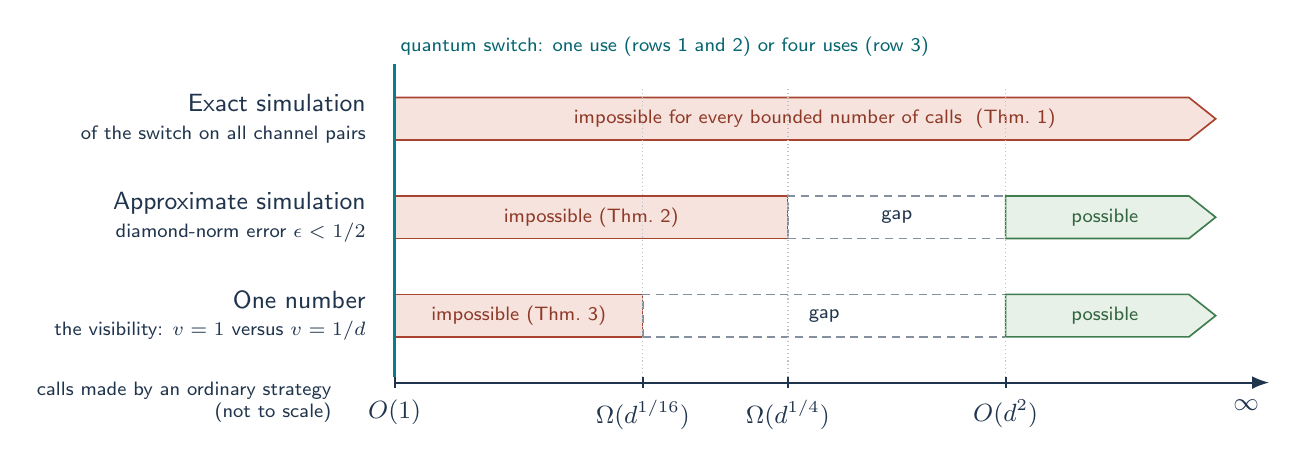
\begin{tikzpicture}[x=.97cm,y=1cm,>=Latex,
 impbar/.style={draw=rust,fill=paleRust,line width=.6pt},
 posbar/.style={draw=leaf,fill=paleLeaf,line width=.6pt},
 opnbar/.style={draw=navy!55,fill=white,line width=.6pt,densely dashed},
 rowlab/.style={font=\small\sffamily,text=navy,align=right,anchor=east},
 inbar/.style={font=\scriptsize\sffamily,text=navy}]
\def\xa{4.5}\def\xb{7.75}\def\xc{9.65}\def\xd{12.5}\def\xe{15.7}
% rows: y centers
\def\ya{2.5}\def\yb{1.25}\def\yc{0}\def\h{.27}
% --- exact ---
\draw[impbar] (\xa,\ya-\h) -- (\xe-.8,\ya-\h) -- (\xe-.45,\ya) -- (\xe-.8,\ya+\h) -- (\xa,\ya+\h) -- cycle;
\node[inbar,text=rust!85!black] at (10.0,\ya) {impossible for every bounded number of calls \ (Thm.~1)};
% --- approximate ---
\draw[impbar] (\xa,\yb-\h) rectangle (\xc,\yb+\h);
\draw[opnbar] (\xc,\yb-\h) rectangle (\xd,\yb+\h);
\draw[posbar] (\xd,\yb-\h) -- (\xe-.8,\yb-\h) -- (\xe-.45,\yb) -- (\xe-.8,\yb+\h) -- (\xd,\yb+\h) -- cycle;
\node[inbar,text=rust!85!black] at ({(\xa+\xc)/2},\yb) {impossible (Thm.~2)};
\node[inbar] at ({(\xc+\xd)/2},\yb) {gap};
\node[inbar,text=leaf!80!black] at ({(\xd+\xe)/2-.3},\yb) {possible};
% --- one number ---
\draw[impbar] (\xa,\yc-\h) rectangle (\xb,\yc+\h);
\draw[opnbar] (\xb,\yc-\h) rectangle (\xd,\yc+\h);
\draw[posbar] (\xd,\yc-\h) -- (\xe-.8,\yc-\h) -- (\xe-.45,\yc) -- (\xe-.8,\yc+\h) -- (\xd,\yc+\h) -- cycle;
\node[inbar,text=rust!85!black] at ({(\xa+\xb)/2},\yc) {impossible (Thm.~3)};
\node[inbar] at ({(\xb+\xd)/2},\yc) {gap};
\node[inbar,text=leaf!80!black] at ({(\xd+\xe)/2-.3},\yc) {possible};
% row labels
\node[rowlab] at (\xa-.25,\ya) {Exact simulation\\[-1pt]{\scriptsize of the switch on all channel pairs}};
\node[rowlab] at (\xa-.25,\yb) {Approximate simulation\\[-1pt]{\scriptsize diamond-norm error $\epsilon<1/2$}};
\node[rowlab] at (\xa-.25,\yc) {One number\\[-1pt]{\scriptsize the visibility: $v=1$ versus $v=1/d$}};
% axis
\draw[figwire,->] (\xa,-.85) -- (\xe+.25,-.85);
\foreach \x/\l in {\xa/{$O(1)$},\xb/{$\Omega(d^{1/16})$},\xc/{$\Omega(d^{1/4})$},\xd/{$O(d^{2})$}}
  {\draw[figwire] (\x,-.78) -- (\x,-.92); \node[figlab,anchor=north] at (\x,-.95) {\l};}
\node[figlab,anchor=north] at (\xe-.05,-.95) {$\infty$};
\node[figtiny,anchor=north east,align=right] at (\xa-.7,-.72) {calls made by an ordinary strategy\\(not to scale)};
% guide lines
\foreach \x in {\xb,\xc,\xd} \draw[draw=navy!30,line width=.4pt,densely dotted] (\x,-.78) -- (\x,\ya+\h+.12);
% the switch marker
\draw[draw=teal,line width=1.1pt] (\xa,-.78) -- (\xa,\ya+\h+.42);
\node[figtiny,text=teal!80!black,anchor=south west] at (\xa-.05,\ya+\h+.4) {quantum switch: one use (rows 1 and 2) or four uses (row 3)};
\end{tikzpicture}
\caption{The three results. Each row is a task that the quantum switch
performs with a constant number of uses, and the axis is the number of
calls made by an ordinary strategy on boxes of dimension $d=2^n$. Red
regions are excluded by Theorems~\ref{thm:exact-simulation},
\ref{thm:simulation-summary} and~\ref{thm:c6}. Green regions are
achievable (Section~\ref{sec:simulation} and
Remark~\ref{rem:crossover}). Dashed regions are the gaps that our
bounds leave undetermined. Exact simulation is only
approached as the number of calls grows. Constants are omitted:
Remarks~\ref{rem:approx-content} and~\ref{rem:crossover} give the sizes
at which the bounds exceed the cost of the switch.}
\label{fig:landscape}
\end{figure}

\paragraph{Exact simulation is impossible with a bounded number of calls.}
An ordinary strategy simulates the switch exactly if it implements
$\SW[A,B]$ for every pair of channels $A,B$.

\begin{theorem}[Exact simulation]\label{thm:exact-simulation}
For every $d\ge2$ and every finite budget $q$, no ordinary strategy with
budget $q$ simulates the switch exactly on $\C^d$, that is, implements
$\SW[A,B]$ for all channels $A,B$ on $\C^d$. This holds even if the
strategy is required to work only for the control input $\ket+$. The
target input is arbitrary, and the output consists of the control and
the target.
\end{theorem}

The theorem proves Conjecture~1 of~\cite{bavaresco2025}. It answers the
question of~\cite{bavaresco2025}, whether a finite number of calls
suffices, in the negative for every bounded number of calls: no
dependence of the budget on $d$ is enough. Three
features of the statement matter. The strategy is fixed first and must
then work for all pairs of channels; this is what a simulation of the
switch as a device means. The order of calls may be chosen adaptively,
so the statement covers every circuit with classical control of causal
order~\cite{wechs2021}; by a recent result~\cite{wechs2026} this class
contains every causally separable process. And the boxes range over all
channels: for unitary boxes three calls suffice, and our proof uses
mixtures of channels in an essential way.

The theorem has three limits. It concerns exact, deterministic
simulation with a bounded number of calls. It does not bound the error
of a strategy with a given budget; arbitrarily good approximations exist
with finitely many calls. It does not exclude heralded simulation, which
succeeds only with some probability~\cite{bavaresco2025}. And it does
not exclude strategies that stop with probability one but have no bound
on their number of calls; this case is open (Section~\ref{sec:open}).


\paragraph{Approximate simulation is expensive.}
The error of a strategy $\QC$ is its largest distance to the switch,
$\operatorname{err}(\QC;d)=\sup_{A,B}\frac12\norm{\QC[A,B]-\SW[A,B]}_\diamond$.

\begin{theorem}[Approximate simulation]\label{thm:simulation-summary}
For $d\ge2$, an ordinary strategy $\QC$ with budget $q$ obeys, for every
integer $r\ge1$,
\begin{equation}\label{eq:tradeoff-intro}
 \operatorname{err}(\QC;d)\ge
 \frac12-\frac{13r^2}{3d}-\frac{q(q-1)}{2r}.
\end{equation}
Thus attaining a fixed error $\epsilon<1/2$ requires
$\Omega_\epsilon(d^{1/4})$ calls. For instance, error at most $1/48$
requires more than $d^{1/4}/8$ calls whenever $d\ge64$. The bound holds
already when the supremum in the error is restricted to pairs of uniform
mixtures of $r$ unitary channels.
\end{theorem}

The integer $r$ is a free parameter. It is the number of unitaries
mixed in each hard box of the proof, and the choice $r\approx\sqrt d$
balances the two negative terms and gives the bound $\Omega(d^{1/4})$.
The value $1/48$ in the example is a convenient choice and not a
threshold: with the same $r$, the bound~\eqref{eq:tradeoff-intro} gives
more than $d^{1/4}/8$ calls for every error up to $71/192$, in
particular for error $1/3$. The threshold $1/2$ is the natural one, since a strategy that
measures the control and then calls the boxes in the corresponding order
has error at most $1/2$ with two calls. In the other direction, about $4d^2/\epsilon$
calls suffice for error $\epsilon$ (Section~\ref{sec:simulation}). At
fixed error the cost of approximate simulation therefore lies between
$d^{1/4}$ and $d^2$, and is exponential in the number of qubits. We do
not claim that the exponent $1/4$ is optimal
(Section~\ref{sec:open}).

\paragraph{A single number is already hard.}
Simulation asks for the whole output of the switch on every input. A common use of the switch asks for much less. Prepare the control in
$\ket+$ and the target in the maximally mixed state, apply the switch,
and measure the control in the basis $\ket\pm$. The outcome $-$ occurs
with probability $(1-v)/2$, where the \emph{visibility}
\[
 v(A,B)=\frac1d\Re\sum_{i,j}\Tr(B_jA_iB_j^\dagger A_i^\dagger)
\]
is computed from Kraus operators $(A_i)$ of $A$ and $(B_j)$ of $B$. The
complement $1-v$ is the squared noncommutativity of $A$ and $B$, a
quantity introduced by Gao et al.~\cite{gao2023}. They used it to
quantify the incompatibility of two measurements and showed that the
switch estimates it with a number of uses that does not depend on the
dimension.

Our third result shows that this one number is exponentially
expensive, in the number of qubits, for ordinary strategies. The hard
instance is the most basic question that the quantity
of~\cite{gao2023} answers: are two measurements the same, or as
incompatible as two measurements can be? The boxes are measurement
devices that do not report their outcomes: each is a \emph{rank-one
dephasing channel}, which measures in a hidden orthonormal basis and
discards the result. For two such channels the visibility lies between
$1/d$ and $1$. It equals $1$ exactly when the two channels coincide; we
call this promise \Same{}. It equals $1/d$ exactly when the two bases
are mutually unbiased; we call this promise \Mub{}.

\begin{theorem}[One number]\label{thm:c6}
Let $d=2^n$, $n\ge1$, and let $A,B$ be rank-one dephasing channels on
$\C^d$.
\begin{enumerate}
\item[\textup{(a)}] \emph{One bit.} Every ordinary strategy that
distinguishes \Same{}, where $v(A,B)=1$, from \Mub{}, where
$v(A,B)=1/d$, with success probability at least $2/3$ on every promised
pair has budget greater than $d^{1/16}/100$. Four independent uses of
the quantum switch suffice: they make eight calls in total and have
one-sided error at most $81/256<1/3$.
\item[\textup{(b)}] \emph{One scalar.} Let $0<\epsilon<1/4$. Every
ordinary strategy that outputs, for every pair $A,B$, an estimate of
$v(A,B)$ that is within $\epsilon$ of the true value with probability
at least $2/3$ has budget greater than $d^{1/16}/100$. With the switch,
$\lceil4/\epsilon^2\rceil$ uses give such an estimate, with probability
at least $1-2e^{-2}>2/3$, for every pair of channels.
\end{enumerate}
\end{theorem}

Part~(b) follows from part~(a), since an estimate within $1/4$ tells the
value $1$ from the value $1/d\le1/2$. Part~(a) says more than a bound on
estimation. The two extreme values of the quantity, which differ by
almost its whole range, cannot be told apart: an ordinary strategy does
not learn even whether the two measurements are the same.

The ordinary strategy in these statements has unbounded quantum memory,
may entangle its queries with that memory, may adapt, and may end with a
collective measurement. What it lacks is the switch, and also any access
to the insides of the boxes: their outcomes, their environments, and the
unitaries that rotate to the hidden bases. Under both promises the two
channels commute: composing them in either order gives the same channel.
The visibility nevertheless differs between the two promises. It is an
interference term between the two orders: it pairs $B_jA_i$ with
$A_iB_j$ for each pair of Kraus operators. Neither composite channel
contains this term.

The separation is asymptotic. The exponent $1/16$ and the constant are
not optimized, and $d^{1/16}/100$ exceeds the eight calls of the switch
test only from $n=155$ qubits on (Remark~\ref{rem:crossover}). For two
copies of the same qubit channel, a four-call circuit that reproduces
the control output of the switch on a fixed input was found numerically
in~\cite{bavaresco2025}; the hardness shown here is an effect of large
dimension. The content of the theorem is that the cost of this one
number grows exponentially with $n$ for ordinary strategies and not at
all for the switch.

The proof of the lower bound given in this paper is complete except for
four structural statements about the recording process of
Section~\ref{sec:c6-proof}. They are listed in
Appendix~\ref{sec:c6-recording} with the reasons they hold, and the
Lean formalization of the theorem does not rely on them
(Appendix~\ref{sec:formal-status}).

\paragraph{Why this number.}
The visibility is what many uses of the switch read out. In each of the
following protocols the control starts in $\ket+$ and is measured in the
basis $\ket\pm$, or in the $Y$ basis for the imaginary counterpart
below. The statistics are those of $v$, with the maximally mixed target
state replaced by the target state of the protocol. For a pair of
unitaries that commute or anticommute, $v$ equals $+1$ or $-1$, so the
switch tells the two cases apart with one call to each
box~\cite{procopio2015,chiribella2012}.
For two measurements, $1-v$ quantifies their
incompatibility~\cite{gao2023}. For two unitaries, $v$ and its imaginary
counterpart give the Bargmann invariants of a set of
states~\cite{azado2025}. For displacements, $v$ is the cosine of the
geometric phase estimated in metrology with indefinite causal
order~\cite{zhao2020}. In switch-assisted
communication~\cite{ebler2018} and refrigeration~\cite{felce2020} the
boxes are known, and the same trace gives the bias of the control
measurement on which those protocols condition. None of these works proves a lower bound on the calls of an ordinary
strategy that grows with the dimension of the boxes. Zhao et
al.~\cite{zhao2020} bound the precision of fixed-order strategies as a
function of the number of uses, not of the dimension. For unitary boxes no large cost is possible, because
three calls reproduce the whole switch. Theorem~\ref{thm:c6} shows that for some irreversible boxes, namely
measurement devices with hidden bases, the number itself is
exponentially expensive for ordinary strategies.

\paragraph{The number at work.}
Section~\ref{sec:validation} gives a use of the number in the
characterization of noise. For a noisy device that applies a channel
$\mathcal E$, the switch with the device in both slots measures the
self-visibility $v(\mathcal E,\mathcal E)$, which is $1$ exactly when
the Kraus operators of $\mathcal E$ commute with one another. A
difference between the measured value and the value predicted by a
noise model $\mathcal M$ certifies that the model is wrong:
$\frac12\norm{\mathcal E-\mathcal M}_\diamond\ge\frac14\lvert
v(\mathcal E,\mathcal E)-v(\mathcal M,\mathcal M)\rvert$
(Proposition~\ref{prop:mismatch}). We then consider noise of strength
$p$ that dephases in a hidden basis and a depolarizing model with the
same average gate fidelity. The switch tells the two apart with
$O(1/p)$ uses of the device, whereas ordinary strategies need
$\Omega(d^{1/16}/p)$ (Corollary~\ref{cor:validation}). Already for two
qubits and two uses the switch beats every ordinary strategy
(Proposition~\ref{prop:two-call}). The same section marks where the hardness ends: a hidden basis from
a short list, and noise that acts on each qubit separately, are easy
for ordinary strategies.

\subsection{Technical overview}\label{sec:overview}

The three theorems have independent proofs. The first two share one
elementary fact: an ordinary
strategy that calls each box at most once uses the boxes in a definite
order on each run. The positive operator that represents such a
strategy (its Choi operator, Section~\ref{sec:ordered}) is therefore a
sum of two positive operators, one for each order
(Lemma~\ref{lem:ordered}).

\paragraph{Exact simulation: polarization and a certificate.}
Suppose a strategy were exact, and pad it with calls on dummy systems
so that every run makes exactly $M$ calls to $A$ and $N$ calls to $B$.
The output of the padded strategy is a polynomial of degree $M$ in $A$
and of degree $N$ in $B$, whereas $\SW[A,B]$ is linear in each.
Exactness on mixtures of channels lets us compare the two sides term by
term (polarization), and shows the following. If one call to each box,
chosen uniformly at random, is kept and every other call is replaced by
the identity channel, the strategy outputs a \emph{diluted switch}
\[
 \tfrac1{MN}\,\SW[A,B]+\tfrac1M\bigl(1-\tfrac1N\bigr)\SW[A,\id]
 +\bigl(1-\tfrac1M\bigr)\tfrac1N\,\SW[\id,B]
 +\bigl(1-\tfrac1M\bigr)\bigl(1-\tfrac1N\bigr)\SW[\id,\id],
\]
with one call to each box. A finite budget has thus been traded for a
small but positive weight on the switch. It remains to show that no
strategy with one call to each box produces a diluted switch, for any
positive weight. For qubits this is a finite problem in linear algebra.
Positivity confines the two operators of Lemma~\ref{lem:ordered}, one
for each order, to an explicit $25$-dimensional space. A linear
functional vanishes on both of them and on every operator that gives
zero on all pairs of channels. On the diluted switch it takes the value
$1/(2MN)$, a contradiction. An embedding of a
qubit extends the contradiction to every dimension
(Section~\ref{sec:exact}, \reffig{fig:exact}).

\paragraph{Approximate simulation: hidden indices and reversed products.}
The hard boxes are uniform mixtures of $r$ Haar-random unitaries,
$A=\frac1r\sum_i\Ad(U_i)$ and $B=\frac1r\sum_j\Ad(V_j)$, where $\Ad(U)$
denotes the channel $\rho\mapsto U\rho U^\dagger$. Each call
applies one of the unitaries, with an index that the strategy never
sees. If $q^2\ll r$ then, with high probability, no index repeats. With
respect to each pair $(U_i,V_j)$ the strategy then calls each box at
most once, in a definite order. The switch, on the other hand, outputs
the superposition
\[
 \tfrac1{\sqrt2}\bigl(\ket0\ket{V_jU_i}+\ket1\ket{U_iV_j}\bigr),
\]
where $\ket W$ denotes the normalized vectorization of a unitary $W$.
We prove that a circuit that calls $U$ before $V$
has average fidelity at most $b_d\approx4/d^2$ with the reversed product
$UV$, so that it can build only a coherence of order $1/d$ between the two orders. A
measurement that detects this coherence then separates the strategy
from the switch. The argument needs $r$ to be at most about $\sqrt d$: each of the
$r^2$ pairs may contribute a coherence of order $1/d$, and the $r^2$
products are orthogonal only up to errors of total size $r^2/d$.
Balancing $r\approx\sqrt d$ against $q^2\ll r$ gives $q=\Omega(d^{1/4})$
(Section~\ref{sec:approximation}, \reffig{fig:approx}).

\paragraph{One number: a cache of rotation-invariant labels.}
A rank-one dephasing channel in the basis given by a unitary $U$ applies
$U^\dagger$, a known dephasing whose outcome stays private, and $U$. We
take $U$ Haar-random and shared by the two boxes, which differ only by a
known rotation of the basis. An ordinary strategy with $q$ calls then
becomes an experiment with $2q$ forward and inverse queries to $U$, and
the path-recording theorem of Ma and Huang~\cite{mahuang2025} replaces
$U$ by a private record of its queries. The entries of this record are
$d$-dimensional registers inside the device, which we call labels; they
are not the indices of the previous paragraph. The main
technical work is to reduce this record to a \emph{label cache}: at each
call the device either retrieves a stored label, dephases it in its own
basis, and stores it again, or creates a fresh, maximally mixed label.
The hidden bases enter only through the dephasing of a retrieved label.
The stored labels are invariant under a common unknown rotation, and we
show that dephasing one of $k$ such labels differs from depolarizing it
by at most $6(k-1)/d$. After every dephasing is replaced by a
depolarization, the cache no longer depends on the two bases. Hence the
two promises produce nearly the same final state. The exponent $1/16$ is inherited from the error of the
recording theorem (Section~\ref{sec:c6-proof}, Figures~\ref{fig:geometry}
and~\ref{fig:cache}). The comparison of the two caches is proved in full
in Section~\ref{sec:c6-proof}. For the reduction to the cache we give a
guide in which every error term is derived
(Appendix~\ref{sec:c6-recording}). Four structural statements listed
there are given with their reasons only; the Lean formalization
establishes the comparison without taking any of them as a hypothesis
(Appendix~\ref{sec:formal-status}).

\subsection{Related work}\label{sec:related}

\paragraph{Simulating the switch.}
That a circuit with a fixed order needs an extra call to simulate the
switch on unitaries goes back to~\cite{chiribella2013}. For the switch
of $N$ unitary gates, ordinary circuits with a number of calls of order
$N^2$ are known~\cite{colnaghi2012,facchini2015}, so for unitary boxes
the cost of ordinary simulation is polynomial. For channels,
Bavaresco et al.~\cite{bavaresco2025} gave the first exponential lower
bound, for circuits that call one of the channels once, excluded several
small budgets for qubits by computer-assisted proofs, and studied
probabilistic and approximate simulation numerically for qubits.
Theorem~\ref{thm:exact-simulation} removes the restrictions on the
budget, and Theorem~\ref{thm:simulation-summary} gives a
dimension-dependent bound for approximation in the diamond norm.
Results of the same kind are known for other transformations of unknown
operations: adding control to an unknown unitary is impossible with any
finite number of calls~\cite{gavorova2024}, whereas inverting it takes
about $d^2$ calls~\cite{odake2025}. Theorem~\ref{thm:exact-simulation}
places the switch on channels in the first category. Two concurrent and independent works~\cite{cheng2026,goldin2026} are
discussed in Section~\ref{sec:concurrent}.

\paragraph{Advantages of indefinite causal order.}
Query advantages of the switch were first found for promise problems on
unknown unitaries~\cite{chiribella2012,araujo2014}. An improved ordinary
algorithm later reduced the gap for the problem of~\cite{araujo2014} to
a logarithmic factor~\cite{renner2021}. Promise problems on qubit gates
with a proved lower bound for causal algorithms were given
in~\cite{renner2022}. For Boolean functions, quantum circuits with
quantum control of causal order, which include the switch, do not reduce
the query complexity~\cite{abbott2024}. More general processes with
indefinite causal order lower the error at a fixed number of
queries~\cite{abbott2024}, and polynomial separations are known for
classical process functions~\cite{abbott2025}. An exponential advantage is known in
communication complexity~\cite{guerin2016}. For discriminating two known
channels, strategies with indefinite order do strictly better at a
finite number of copies~\cite{bavaresco2021} but have the same Stein
exponent as strategies with definite order~\cite{zhuwang2026}. Our third theorem is a query
separation for unknown irreversible channels against ordinary strategies
with unrestricted memory.

\paragraph{The visibility.}
Gao et al.~\cite{gao2023} introduced the statistic, its estimator with
the switch, and its interpretation for measurements; they also noted
that it can be estimated by ordinary means if the outcomes of the
measurements are available. We prove that without the outcomes the number of ordinary calls must
grow with the dimension, at least as $d^{1/16}$. For two rank-one dephasing channels, $1-v$ equals the mutual
averaged noncommutativity of the two maximal abelian algebras in the
sense of Zanardi~\cite{zanardi2024}, and $v$ has the algebraic form of an infinite-temperature
out-of-time-order correlator of two phase-randomized unitaries, without
any time evolution (Appendix~\ref{sec:connections}).

\paragraph{Techniques.}
The lower bound for the visibility builds on the path-recording
framework for Haar-random unitaries with forward and inverse
queries~\cite{mahuang2025}. Our contribution there is the reduction of
the shared recording process to a trace-preserving cache and the control
of the information in that cache. All results are about oracle queries.
The hard boxes are built from Haar-random unitaries and cannot be
implemented efficiently. Appendix~\ref{sec:connections} gives a version
with efficiently implementable boxes, under a cryptographic
assumption.

\paragraph{Organization.}
Section~\ref{sec:framework} defines the model.
Sections~\ref{sec:exact}, \ref{sec:approximation}
and~\ref{sec:c6-proof} prove the three theorems.
Section~\ref{sec:discussion} discusses where such black boxes arise,
lists open problems, and compares with concurrent work. The appendices
contain the remaining technical parts of the proofs, an application
under an explicit promise, and the scope of the formal verification.

\section{Framework}\label{sec:framework}

This section fixes the objects that the three theorems are about: black
boxes, the quantum switch, ordinary strategies and how their calls are
counted, the two notions of simulation, and the number that the switch
reads off its control qubit.

\subsection{Black boxes}

A \emph{black box} is a device that implements a fixed quantum channel,
that is, a completely positive trace-preserving (CPTP) map $A$ on the
operators of $\C^d$. One \emph{call} applies $A$ to a $d$-dimensional
system chosen by the user, who may keep that system entangled with
anything else. The device has no memory, so different calls act
independently. Only this input--output action is available. If
$A(\rho)=\sum_iA_i\rho A_i^\dagger$ for Kraus operators $(A_i)$, then
the index $i$, the environment in any dilation of $A$, and any classical
outcome produced inside the device stay hidden. When $A$ describes a
measurement, the outcome is not reported.

\subsection{The quantum switch}

Let $A$ and $B$ be channels on $\C^d$ with Kraus operators $(A_i)$ and
$(B_j)$. The \emph{quantum switch}~\cite{chiribella2013} is the channel
$\SW[A,B]$ on a control qubit and a $d$-dimensional target with Kraus
operators
\begin{equation}\label{eq:switch}
 K_{ij}=\proj0\otimes B_jA_i+\proj1\otimes A_iB_j.
\end{equation}
The channel $\SW[A,B](\omega)=\sum_{i,j}K_{ij}\,\omega K_{ij}^\dagger$
does not depend on the Kraus operators chosen to represent $A$ and
$B$~\cite{chiribella2013}, so that it is defined for black boxes, and it
is linear in $A$ and in $B$ separately. If the control is in the state $\ket0$ the target undergoes
$B\circ A$, and if it is in the state $\ket1$ the target undergoes
$A\circ B$. A superposition of the two control states leaves the control
and the target in a state that carries interference between the ordered
products $B_jA_i$ and $A_iB_j$. One use of the switch makes one call to each of the two boxes.

\subsection{Ordinary strategies}\label{sec:model}

The competitor is a quantum circuit with classical control of causal
order in the sense of~\cite{wechs2021}, in which a box may fill several
slots. We call it an ordinary strategy.

\begin{definition}[Ordinary strategy]\label{def:ordinary}
An \emph{ordinary strategy} with \emph{budget} $q$ consists of an input
system, which may be trivial, a query system of dimension $d$, a quantum
memory of arbitrary finite dimension, and known quantum instruments
$W_0,\dots,W_q$ that act on the query system and the memory. The
instrument $W_0$ also receives the input, and $W_t$ may depend on the
outcomes of $W_0,\dots,W_{t-1}$. After $W_t$, the outcomes of $W_0,\dots,W_t$
determine whether the strategy stops and returns a designated output
system, or calls a box on the query system, and which of $A$ and $B$ it
calls.
Every sequence of outcomes leads to at most $q$ calls. The channel
$\QC[A,B]$ that the strategy implements, from its input to its output,
is the sum over all sequences of outcomes: nothing is postselected. The
same definition applies to any finite set of boxes.
\end{definition}

\reffig{fig:switch}(b) shows one run. The definition gives the strategy
arbitrary entangled memory, arbitrary known operations between calls,
adaptive choice of the next box, early stopping, and a collective final
measurement. Circuits with a fixed order of calls, also called quantum
combs, are the special case in which the choice of the next box does not
depend on the outcomes.
Known operations may be controlled coherently. What the strategy cannot
do is put the choice of the unknown box into superposition. The budget
counts calls to $A$ and to $B$ together, on the worst run.

For simulation, the input and the output are a control qubit and a
target. For the tasks of Theorem~\ref{thm:c6} the input is trivial and
the output is a classical guess. A circuit with $k_A$ slots for $A$ and
$k_B$ slots for $B$, as in~\cite{bavaresco2025}, is an ordinary strategy
with budget $k_A+k_B$. Conversely, an ordinary strategy with budget $q$
can be padded, by calls on discarded systems, so that every run makes
exactly $q$ calls to each box (Section~\ref{sec:polarization}); the
order of the calls remains adaptive.

\subsection{Simulating the switch}

An ordinary strategy with a control qubit and a target as input and as
output \emph{simulates the switch exactly} if $\QC[A,B]=\SW[A,B]$ for
every pair of channels $A,B$ on $\C^d$. Its \emph{error} is the largest
distance to the switch over all pairs of boxes,
\begin{equation}\label{eq:simulation-error}
 \operatorname{err}(\QC;d)=
 \sup_{A,B\ \mathrm{CPTP}}\frac12\norm{\QC[A,B]-\SW[A,B]}_\diamond .
\end{equation}
The diamond norm allows the input to be entangled with a reference, so
that $\operatorname{err}(\QC;d)$ is the largest difference, over all
pairs of boxes and all tests, between the probabilities with which a
single test accepts the strategy and accepts the switch.
Both notions ask for the full output, control and target together, on
every input.

\subsection{The visibility}\label{sec:visibility}

The simplest experiment with the switch prepares the control in
$\ket+=(\ket0+\ket1)/\sqrt2$ and the target in the maximally mixed
state $I/d$, and measures the Pauli observable $X$ on the control. From
\eqref{eq:switch}, its expectation value is
\begin{equation}\label{eq:visibility}
 v(A,B)=\frac1d\Re\sum_{i,j}\Tr(B_jA_iB_j^\dagger A_i^\dagger).
\end{equation}
We call $v(A,B)$ the \emph{visibility} of the pair. The outcomes $+$ and
$-$ occur with probabilities $(1\pm v)/2$. The visibility is the
interference statistic of Gao et al.~\cite{gao2023}, with
$1-v=\operatorname{NCOM}_{I/d}^2$ in their notation. It equals $1$ when
every $A_i$ commutes with every $B_j$, and in general
$1-v=\frac1{2d}\sum_{i,j}\norm{[A_i,B_j]}_{\rm HS}^2$. For projective
measurements $1-v$ vanishes exactly when the two measurements are
compatible; for general instruments it quantifies the noncommutativity
of the Kraus operators.

The boxes in our third theorem are measurements with unread outcomes.
For an orthonormal basis $\mathcal B=(b_j)_{j=1}^d$ of $\C^d$, write
\[
 \Delta_{\mathcal B}(\rho)=\sum_j P_j\rho P_j,
 \qquad P_j=\proj{b_j},\qquad \Omega(\rho)=I\Tr(\rho)/d.
\]
The channel $\Delta_{\mathcal B}$ is a \emph{rank-one dephasing
channel}: it measures in the basis $\mathcal B$ and discards the
outcome. The channel $\Omega$ is completely depolarizing. For two such boxes,
with bases $(b_j)$ and $(c_k)$,
\begin{equation}\label{eq:basis-visibility}
 v(\Delta_{\mathcal B},\Delta_{\mathcal C})
 =\frac1d\sum_{j,k}|\langle b_j,c_k\rangle|^4 .
\end{equation}
Two dephasing channels satisfy the promise \Same{} if they coincide as
channels, and the promise \Mub{} if their bases are mutually unbiased,
$|\langle b_j,c_k\rangle|^2=1/d$ for all $j,k$. The visibility is $1$
under \Same{} and $1/d$ under \Mub{}. Under \Same{} either composition
of the two channels is $\Delta_{\mathcal B}$, and under \Mub{} either
composition is $\Omega$. The two channels therefore commute under both
promises. The visibility detects interference between the Kraus
operators of the two boxes. The two composite channels are equal and do
not contain it.

\subsection{Strategies that call each box once}\label{sec:ordered}

The switch calls each box once. An ordinary strategy that also calls
each box at most once must call them in one order or the other on each
run. The following standard fact~\cite{wechs2021} makes this precise and
is used in the proofs of Theorems~\ref{thm:exact-simulation}
and~\ref{thm:simulation-summary}. It is stated for Choi operators, which we now define.

Consider a strategy with input system $P$ and output system $F$ that
calls each box exactly once, appending a call on a discarded system
where one is missing. Let the two calls have input and output systems
$A_I,A_O$ and $B_I,B_O$. Fix a sequence $\alpha$ of outcomes and Kraus
indices of the instruments. The corresponding product of Kraus operators
is a tensor $v_\alpha$ on $P\otimes A_I\otimes A_O\otimes B_I\otimes
B_O\otimes F$. When the boxes have Kraus operators $(A_i)$ and $(B_j)$,
the strategy has Kraus operators $\mathcal L(A_i,B_j)v_\alpha$, where
the \emph{link} $\mathcal L$ contracts the first box with the legs
$A_I,A_O$ and the second with the legs $B_I,B_O$:
\[
 [\mathcal L(K,K')v]_{p,f}
 =\sum_{a,a',b,b'}v_{p,a,a',b,b',f}\,K_{a',a}K'_{b',b},
\]
without complex conjugation. (The Kraus vectors $v_\alpha$ are not
related to the visibility $v(A,B)$.) The \emph{Choi operator} of the strategy
is $C=\sum_\alpha v_\alpha v_\alpha^\dagger$, and we call the $v_\alpha$
its \emph{Kraus vectors}. It is a positive semidefinite operator that
determines $\QC[A,B]$ for all $A,B$, linearly in $A$ and in $B$. The
same definition applies to any process whose Kraus operators are
bilinear in the Kraus operators of the two boxes, such as the switch.

\begin{lemma}[Ordered components]\label{lem:ordered}
Let $\QC$ be an ordinary strategy that calls $A$ at most once and $B$ at
most once on every run. Then its Choi operator is a sum
\[
 C=C_{A\before B}+C_{B\before A}
\]
of two positive semidefinite operators. The first satisfies the
homogeneous comb equations of a circuit that calls $A$ before $B$,
\begin{equation}\label{eq:ordered-comb}
\begin{aligned}
 d\,\Tr_F C_{A\before B}&=\bigl(\Tr_{B_OF}C_{A\before B}\bigr)\otimes I_{B_O},\\
 d\,\Tr_{B_IB_OF} C_{A\before B}&=\bigl(\Tr_{A_OB_IB_OF}C_{A\before B}\bigr)\otimes I_{A_O},
\end{aligned}
\end{equation}
and the second satisfies the same equations with the roles of $A$ and
$B$ exchanged. For a fixed input state, the first call is to $A$ with a
probability $p_{A\before B}$ and to $B$ with probability
$p_{B\before A}=1-p_{A\before B}$, and these probabilities do not
depend on the boxes.
\end{lemma}

\begin{proof}
Append any missing call on a discarded register, so that every run calls
both boxes. Group the runs by the box that is called first. Everything
that happens before the first call is known processing, so this grouping
is the outcome of an instrument that does not depend on the boxes; for a
fixed input state its two outcomes have probabilities
$p_{A\before B}+p_{B\before A}=1$. Given the outcome, the remaining
circuit calls the two boxes in a fixed order, with arbitrary memory in
between. Summing its Kraus vectors over all later outcomes gives a Choi
operator that is positive and obeys the comb equations of that
order~\cite{wechs2021}. The equations in~\eqref{eq:ordered-comb}
are homogeneous because the weight of each group may depend on the input
state, so neither component need be normalized on its own.
\end{proof}

Later instruments of the strategy can split a component further. If
$C_{\rm out}$ is the part of a component selected by some later outcome,
then $0\preceq C_{\rm out}\preceq C_{A\before B}$, and $C_{\rm out}$ need
not satisfy~\eqref{eq:ordered-comb} itself. We call $C_{A\before B}$ the
\emph{completed parent} of $C_{\rm out}$. This notion is used in
Lemma~\ref{lem:reverse} and in the proof of
Corollary~\ref{cor:coherence}.

\section{Exact simulation: no bounded number of calls suffices}\label{sec:exact}

We prove Theorem~\ref{thm:exact-simulation}. The proof has three steps,
shown in \reffig{fig:exact}. First, an exact simulator with any finite
budget is converted into an ordinary strategy that calls each box
\emph{once} and outputs a diluted switch, a mixture in which the switch
appears with a small but positive weight. Second, a strategy that calls
each box once is a sum of two components with definite orders
(Lemma~\ref{lem:ordered}). Third, for qubits a linear functional
separates every such sum from the diluted switch. An embedding then
extends the qubit contradiction to every dimension.

\begin{figure}[!b]
\centering
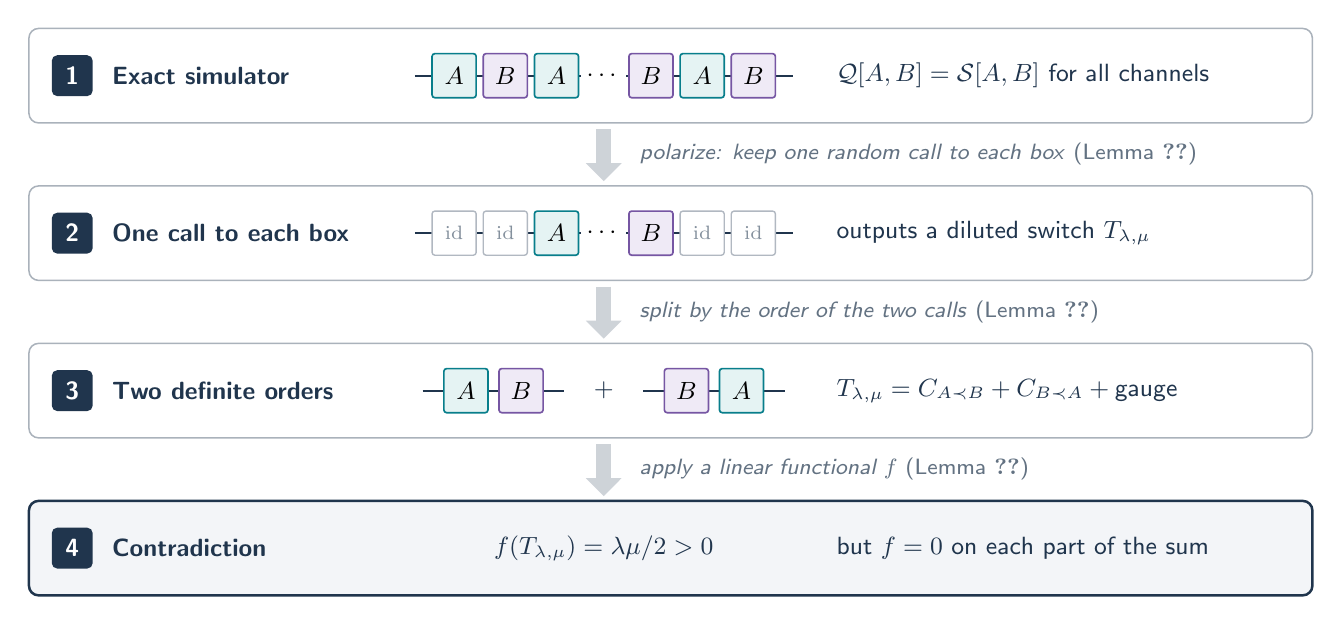
\begin{tikzpicture}[x=1cm,y=1cm]
\def\H{1.2}\def\W{16.3}
%% rows (top to bottom)
\foreach \y/\k/\nm in {6.0/1/{Exact simulator},4.0/2/{One call to each box},2.0/3/{Two definite orders}}{
 \draw[flowbox] (0,\y) rectangle (\W,\y+\H);
 \node[flowtab] at (.55,\y+.6) {\k};
 \node[flowname] at (1.05,\y+.6) {\nm};}
\draw[flowend] (0,0) rectangle (\W,\H);
\node[flowtab] at (.55,.6) {4};
\node[flowname] at (1.05,.6) {Contradiction};
%% arrows between rows, with the proof step that they stand for
\foreach \y/\t in {6.0/{polarize: keep one random call to each box \textup{(Lemma~\ref{lem:polarization})}},
                   4.0/{split by the order of the two calls \textup{(Lemma~\ref{lem:ordered})}},
                   2.0/{apply a linear functional $f$ \textup{(Lemma~\ref{lem:exact-obstruction})}}}{
 \draw[flowdown] (7.3,\y-.08) -- (7.3,\y-.74);
 \node[flowstep] at (7.75,\y-.4) {\t};}
%% row 1: a strategy with many calls
\draw[figwire] (4.9,6.6) -- (9.7,6.6);
\foreach \x/\s/\l in {5.4/fsA/A,6.05/fsB/B,6.7/fsA/A,7.9/fsB/B,8.55/fsA/A,9.2/fsB/B} \node[\s] at (\x,6.6) {$\l$};
\node[fill=white,inner sep=2pt,font=\small] at (7.3,6.6) {$\cdots$};
\node[flownote] at (10.25,6.6) {$\QC[A,B]=\SW[A,B]$ for all channels};
%% row 2: all calls but one to each box replaced by the identity
\draw[figwire] (4.9,4.6) -- (9.7,4.6);
\foreach \x/\s/\l in {5.4/fsI/\mathrm{id},6.05/fsI/\mathrm{id},6.7/fsA/A,7.9/fsB/B,8.55/fsI/\mathrm{id},9.2/fsI/\mathrm{id}} \node[\s] at (\x,4.6) {$\l$};
\node[fill=white,inner sep=2pt,font=\small] at (7.3,4.6) {$\cdots$};
\node[flownote] at (10.25,4.6) {outputs a diluted switch $T_{\lambda,\mu}$};
%% row 3: the two ordered parts
\draw[figwire] (5.0,2.6) -- (6.8,2.6); \node[fsA] at (5.55,2.6) {$A$}; \node[fsB] at (6.25,2.6) {$B$};
\node[font=\small,text=navy] at (7.3,2.6) {$+$};
\draw[figwire] (7.8,2.6) -- (9.6,2.6); \node[fsB] at (8.35,2.6) {$B$}; \node[fsA] at (9.05,2.6) {$A$};
\node[flownote] at (10.25,2.6) {$T_{\lambda,\mu}=C_{A\before B}+C_{B\before A}+{}$gauge};
%% row 4: the two evaluations of f
\node[font=\small,text=navy] at (7.3,.6) {$f(T_{\lambda,\mu})=\lambda\mu/2>0$};
\node[flownote] at (10.25,.6) {but $f=0$ on each part of the sum};
\end{tikzpicture}
\caption{The proof of Theorem~\ref{thm:exact-simulation} as a chain of
four statements; each arrow is one step of the proof. Row~1: suppose an
ordinary strategy reproduced the switch exactly, with $M$ calls to $A$
and $N$ calls to $B$. Row~2: because the strategy must work for all
channels, including mixtures, one may keep one call to each box, chosen
at random, and give every other call the identity channel. The result
is a diluted switch, a mixture in which the switch has weight
$\lambda\mu=1/(MN)$. Row~3: a strategy that calls each box once is a
sum of two parts with definite orders, up to the \emph{gauge}, the
operators that give zero on every pair of channels. Row~4: for qubits,
a linear functional $f$ vanishes on both parts and on the gauge but is
strictly positive on every diluted switch.}
\label{fig:exact}
\end{figure}

\subsection{From many calls to one call each}\label{sec:polarization}

Suppose that an ordinary strategy $\QC$ with budget $q$ simulates the
switch exactly on $\C^d$.

\paragraph{Normal form.}
A call made on a discarded dummy system does not change the channel that
a strategy implements. Appending such calls, we may assume that every
run makes exactly $M$ calls to $A$ and exactly $N$ calls to $B$, with
$M=N=q$. We keep two letters because the two boxes play separate roles
below.

\paragraph{Slot channels.}
On each run, number the calls to $A$ in the order in which they are
made, and likewise the calls to $B$. Now let the $k$th call to $A$ apply
a channel $A^{(k)}$ and the $l$th call to $B$ apply a channel $B^{(l)}$,
where $A^{(1)},\dots,A^{(M)}$ and $B^{(1)},\dots,B^{(N)}$ are arbitrary
channels on $\C^d$. (Superscripts label slots; the subscripts $i,j$ label Kraus operators.) This defines a channel
$\QC(A^{(1)},\dots,A^{(M)};B^{(1)},\dots,B^{(N)})$ that is linear in each
of its $M+N$ arguments, because each of them is used exactly once on
every run. Permuting the labels of the $A$-slots and those of the
$B$-slots uniformly at random before the computation gives a strategy
$\QC_{\mathrm{sym}}$ that is, in addition, symmetric in its first $M$
arguments and in its last $N$ arguments. It is still an ordinary
strategy: the relabelling is classical randomness, and the adaptive
choice of the next box is untouched. When all $A^{(k)}$ equal $A$ and
all $B^{(l)}$ equal $B$ the relabelling has no effect, so
$\QC_{\mathrm{sym}}(A,\dots,A;B,\dots,B)=\QC[A,B]=\SW[A,B]$.

\begin{lemma}[Polarization]\label{lem:polarization}
For all channels $A^{(1)},\dots,A^{(M)}$ and $B^{(1)},\dots,B^{(N)}$ on
$\C^d$,
\begin{equation}\label{eq:polarization}
 \QC_{\mathrm{sym}}\bigl(A^{(1)},\ldots,A^{(M)};B^{(1)},\ldots,B^{(N)}\bigr)
 =\frac1{MN}\sum_{k=1}^{M}\sum_{l=1}^{N}\SW\bigl[A^{(k)},B^{(l)}\bigr].
\end{equation}
\end{lemma}

\begin{proof}
Let $x=(x_1,\dots,x_M)$ and $y=(y_1,\dots,y_N)$ be probability vectors.
The mixtures $\sum_kx_kA^{(k)}$ and $\sum_ly_lB^{(l)}$ are channels, so
the strategy is exact on them. Insert them in every slot and expand both
sides, using the multilinearity of $\QC_{\mathrm{sym}}$ and the
bilinearity of the switch:
\[
 \sum_{\substack{k_1,\dots,k_M\\ l_1,\dots,l_N}}
 x_{k_1}\!\cdots x_{k_M}\,y_{l_1}\!\cdots y_{l_N}\;
 \QC_{\mathrm{sym}}\bigl(A^{(k_1)},\ldots,A^{(k_M)};B^{(l_1)},\ldots,B^{(l_N)}\bigr)
 =\sum_{k,l}x_ky_l\,\SW\bigl[A^{(k)},B^{(l)}\bigr].
\]
Multiply the right side by
$(\sum_kx_k)^{M-1}(\sum_ly_l)^{N-1}=1$. Both sides are now polynomials
that are homogeneous of degree $M$ in $x$ and of degree $N$ in $y$. They
agree on the product of the two simplices, hence on the product of the
two positive cones by homogeneity, hence identically. Compare the
coefficients of $x_1\cdots x_M\,y_1\cdots y_N$. On the left it is
$M!\,N!\,\QC_{\mathrm{sym}}(A^{(1)},\ldots,A^{(M)};B^{(1)},\ldots,B^{(N)})$,
by symmetry. On the right it is
$(M-1)!\,(N-1)!\sum_{k,l}\SW[A^{(k)},B^{(l)}]$. Dividing
gives~\eqref{eq:polarization}.
\end{proof}

\paragraph{Dilution.}
In~\eqref{eq:polarization}, put the unknown channel $A$ in one $A$-slot
and the identity channel in the other $M-1$, and do the same for $B$.
Because $\QC_{\mathrm{sym}}$ permutes the slots at random, this keeps a
uniformly random call to each box.
The identity channels are known operations and can be absorbed into the
strategy. What remains is an ordinary strategy that calls $A$ once and
$B$ once and implements
\begin{equation}\label{eq:dilution}
\begin{split}
 T_{\lambda,\mu}(A,B)={}&\lambda\mu\,\SW[A,B]
 +\lambda(1-\mu)\,\SW[A,\id]\\
 &+(1-\lambda)\mu\,\SW[\id,B]
 +(1-\lambda)(1-\mu)\,\SW[\id,\id],
\end{split}
\end{equation}
with $\lambda=1/M>0$ and $\mu=1/N>0$. We call $T_{\lambda,\mu}$ a
\emph{diluted switch}. The switch itself appears in it with weight
$\lambda\mu=1/(MN)$, which is small for a large budget but never zero.

\begin{remark}[Channels are essential]\label{rem:unitary}
The polarization step evaluates the simulator on mixtures of channels,
which are channels. The set of unitary channels is not convex, and for
unitary boxes the conclusion of Theorem~\ref{thm:exact-simulation} is
false. \reffig{fig:unitary} shows a circuit with three calls. If the
control is $\ket1$, swap the target with a dummy system prepared in a
fixed pure state, call $A$, and undo the swap. Call $B$ on the target. If the control is $\ket0$, swap
the target with the dummy, call $A$ a second time, and undo the swap. On
either branch the target undergoes the two boxes in the right order and
the dummy undergoes $A$ once. When $A$ is unitary the dummy ends in the
same pure state on both branches and factors out, so three calls
reproduce the switch exactly on all pairs of
unitaries~\cite{chiribella2013}. When $A$ is a channel, its two calls
have independent Kraus indices, whereas the switch needs the same index
on both branches. The dummy becomes correlated with the control, the
coherence of the control is reduced, and the output differs from the
switch.
\end{remark}

\begin{figure}[t]
\centering
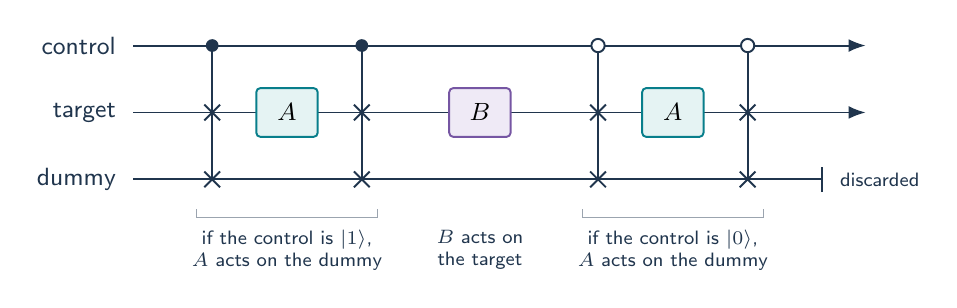
\begin{tikzpicture}[x=1cm,y=1cm,>=Latex,
 ctl/.style={circle,fill=navy,inner sep=0pt,minimum size=4.6pt},
 octl/.style={circle,draw=navy,fill=white,line width=.7pt,inner sep=0pt,minimum size=4.8pt}]
\def\swapx#1#2{\draw[figwire] (#1-.1,#2-.1) -- (#1+.1,#2+.1) (#1-.1,#2+.1) -- (#1+.1,#2-.1);}
\draw[figwire,->] (0,1.7) -- (9.3,1.7);
\draw[figwire,->] (0,.85) -- (9.3,.85);
\draw[figwire] (0,0) -- (8.75,0);
\draw[figwire] (8.75,-.16) -- (8.75,.16);
\node[figlab,anchor=east] at (-.1,1.7) {control};
\node[figlab,anchor=east] at (-.1,.85) {target};
\node[figlab,anchor=east] at (-.1,0) {dummy};
\node[figtiny,anchor=west] at (8.85,0) {discarded};
\foreach \x in {1.0,2.9} {\draw[figwire] (\x,1.7) -- (\x,0); \node[ctl] at (\x,1.7) {}; \swapx{\x}{.85} \swapx{\x}{0}}
\foreach \x in {5.9,7.8} {\draw[figwire] (\x,1.7) -- (\x,0); \node[octl] at (\x,1.7) {}; \swapx{\x}{.85} \swapx{\x}{0}}
\node[gateA] at (1.95,.85) {$A$};
\node[gateB] at (4.4,.85) {$B$};
\node[gateA] at (6.85,.85) {$A$};
\draw[draw=navy!45,line width=.5pt] (.8,-.38) -- (.8,-.48) -- (3.1,-.48) -- (3.1,-.38);
\draw[draw=navy!45,line width=.5pt] (5.7,-.38) -- (5.7,-.48) -- (8.0,-.48) -- (8.0,-.38);
\node[figtiny,anchor=north] at (1.95,-.52) {if the control is $\ket1$,\\$A$ acts on the dummy};
\node[figtiny,anchor=north] at (4.4,-.52) {$B$ acts on\\the target};
\node[figtiny,anchor=north] at (6.85,-.52) {if the control is $\ket0$,\\$A$ acts on the dummy};
\end{tikzpicture}
\caption{Three calls simulate the switch on unitary boxes. Controlled
swaps send the first call to $A$ to the target if the control is
$\ket0$ and to a dummy system if it is $\ket1$, and the second call the
other way round. The target undergoes $A$ then $B$ on the first branch
and $B$ then $A$ on the second, and the dummy undergoes $A$ once on
either branch. A unitary $A$ leaves the dummy in the same pure state on
both branches. A channel $A$ does not: its two calls act with
independent Kraus operators, and the dummy partly records which branch
was taken.}
\label{fig:unitary}
\end{figure}

\subsection{One call each means a definite order}

Fix the control input of the strategy obtained above to $\ket+$. Its
input $P$ is then the target, and its output $F=F_c\otimes F_t$ consists
of the control and the target. By Lemma~\ref{lem:ordered} its Choi
operator is a sum $C_{A\before B}+C_{B\before A}$ of two positive
operators that obey the homogeneous comb equations of their orders. The
input-dependent weights of the two orders play no role in what follows:
only positivity and the homogeneous equations~\eqref{eq:ordered-comb}
are used.

\subsection{A linear certificate for qubits}\label{sec:qubit-certificate}

Let $d=2$, so that $P,A_I,A_O,B_I,B_O,F_c,F_t$ are qubits. A Kraus
vector of an ordered component, in the sense of
Section~\ref{sec:ordered}, is a vector $v\in\C^{128}$ on these seven
factors. Inserting unitary boxes $U$ and $V$ maps it to a vector on
$P\otimes F_c\otimes F_t$ by the link of Section~\ref{sec:ordered},
which now reads
\begin{equation}\label{eq:vector-link}
 [\mathcal L(U,V)v]_{pct}
 =\sum_{a_i,a_o,b_i,b_o}
 v_{p,a_i,a_o,b_i,b_o,c,t}\,U_{a_o,a_i}V_{b_o,b_i}.
\end{equation}
There is no complex conjugation in this convention.

\paragraph{Support.}
Let $\mathcal H(U,V)$ be the span of the vectorizations of $\ket+I$,
$\ket+U$, $\ket+V$, and $(\ket0VU+\ket1UV)/\sqrt2$, with the factors
ordered as in~\eqref{eq:vector-link}. These are the Kraus operators of
the four terms of~\eqref{eq:dilution} on unitary boxes, so for unitary
boxes the Choi operator of the channel $T_{\lambda,\mu}(U,V)$ is
supported on $\mathcal H(U,V)$. Define the \emph{universal support}
\[
 \mathcal V=\{v:\mathcal L(U,V)v\in\mathcal H(U,V)
                    \text{ for all qubit unitaries }U,V\}.
\]
Every Kraus vector $v_\alpha$ of $C_{A\before B}$ and of
$C_{B\before A}$ lies in $\mathcal V$. Indeed, for
$w\perp\mathcal H(U,V)$, equality with the diluted switch gives
$\sum_\alpha|\langle w,\mathcal L(U,V)v_\alpha\rangle|^2=0$, where the
sum runs over the Kraus vectors of both components. Both components
are positive, so the sum has only nonnegative terms, and support
outside $\mathcal H(U,V)$ cannot cancel between them. Hence every
summand vanishes.

The lemma below refers to one particular Choi operator for the diluted
switch. Let $C_T$ be the Choi operator, in the convention of
Section~\ref{sec:ordered}, of the following process with one slot for
each box and control input $\ket+$. With probabilities $\lambda\mu$,
$\lambda(1-\mu)$, $(1-\lambda)\mu$ and $(1-\lambda)(1-\mu)$ it applies
the switch to $(A,B)$, $(A,\id)$, $(\id,B)$ and $(\id,\id)$, and it
sends a maximally mixed dummy state through each box that it does not
use. This process implements $T_{\lambda,\mu}(A,B)$ for all channels
$A,B$.

\begin{lemma}[Finite qubit obstruction]\label{lem:exact-obstruction}
The support $\mathcal V$ is the range of an explicit full-column-rank integer
matrix $E\in\mathbb Z^{128\times25}$. On real symmetric coordinate matrices
$X\in\mathbb R^{25\times25}$, there is a linear
functional $f$ with the following properties. It vanishes when $EXE^T$
satisfies either set of homogeneous comb
equations~\eqref{eq:ordered-comb}. It vanishes when $EXE^T$ lies in the
CPTP gauge (the subspace of operators that give zero on every pair of
channels).
The operator $C_T$ defined above has the form $C_T=EX_TE^T$, and
$f(X_T)=\lambda\mu/2$ for all $\lambda,\mu\in[0,1]$.
\end{lemma}

Appendix~\ref{sec:certificate} gives $E$, $f$ and $X_T$ explicitly and
states the three exact-arithmetic checks that prove the lemma. The data
for these checks are part of the supplementary material, and the checks
are also part of the Lean formalization
(Appendix~\ref{sec:formal-status}).

\paragraph{Coordinates.}
Write the two components as $C_{A\before B}=EX_{AB}E^T$ and
$C_{B\before A}=EX_{BA}E^T$; recall that $E$ is real. Since $E$ has full column rank and
both components are supported on its range, $X_{AB}$ and $X_{BA}$ are
Hermitian and positive semidefinite. Averaging each with its entrywise
complex conjugate makes them real symmetric and preserves the comb
equations and the equality with the diluted switch, because $E$, the
equations, and $C_T$ are real.

\paragraph{Gauge.}
The strategy agrees with the diluted switch on channels only, so the two
Choi operators need not be equal. For a subsystem $S$, write
${}_SC=(I_S/\dim S)\otimes\Tr_SC$, with the original order of the
factors restored, and set
\[
 \Lambda_A(C)=C-{}_{A_O}C+{}_{A_IA_O}C,\qquad
 \Lambda_B(C)=C-{}_{B_O}C+{}_{B_IB_O}C .
\]
These are projections whose ranges
are spanned by the Choi operators of channels
(Appendix~\ref{sec:certificate}). The kernel of $\Lambda_A\Lambda_B$ is
the \emph{gauge}: the operators that give zero on every pair of
channels. Equality of the strategy and the diluted switch on all pairs
of channels is therefore the single linear equation
\[
 \Lambda_A\Lambda_B\bigl(E(X_{AB}+X_{BA}-X_T)E^T\bigr)=0 .
\]

\paragraph{Contradiction.}
Lemma~\ref{lem:exact-obstruction} gives $f(X_{AB})=f(X_{BA})=0$ from the
comb equations and $f(X_{AB}+X_{BA}-X_T)=0$ from the gauge. Hence
$f(X_T)=0$. But $f(X_T)=\lambda\mu/2=1/(2MN)>0$. Hence no ordinary
strategy with a bounded budget simulates the qubit switch exactly, even
when the control input is fixed to the state $\ket+$.

\begin{figure}[t]
\centering
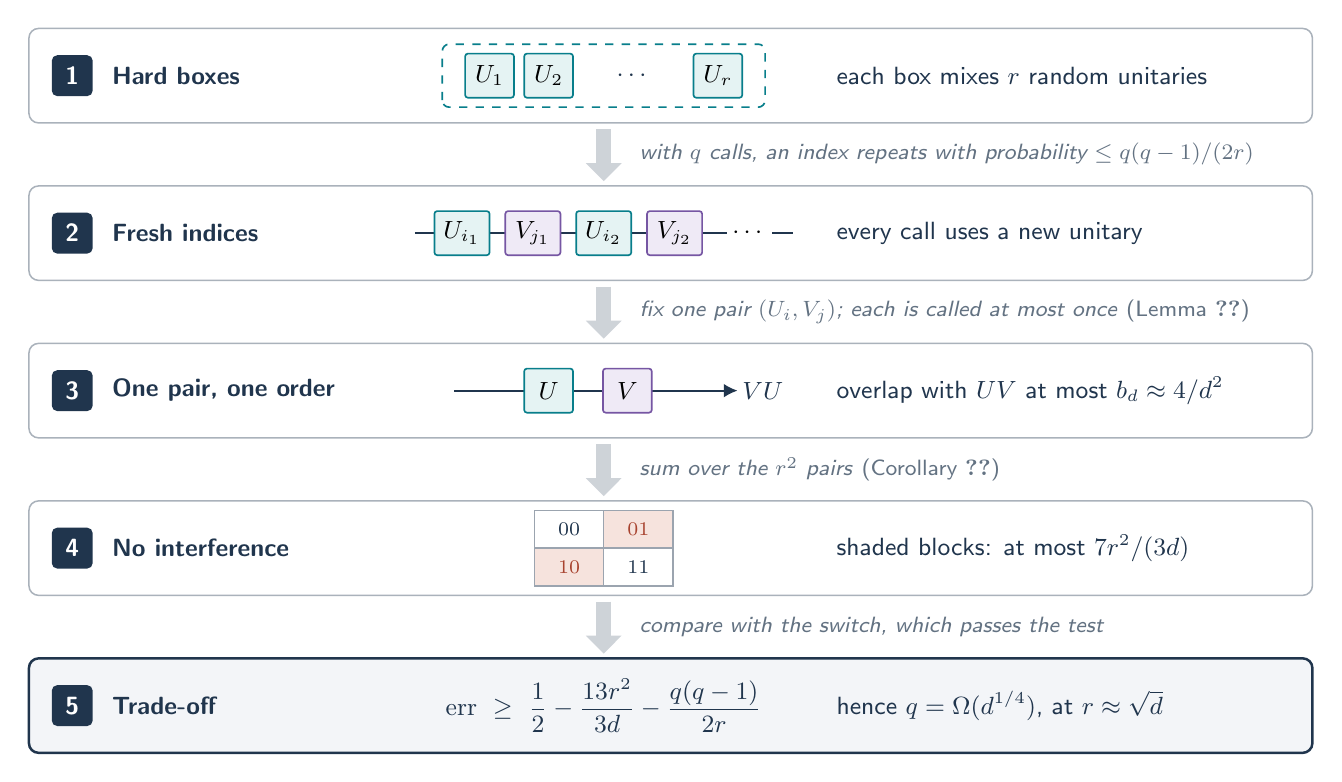
\begin{tikzpicture}[x=1cm,y=1cm]
\def\H{1.2}\def\W{16.3}
\foreach \y/\k/\nm in {8.0/1/{Hard boxes},6.0/2/{Fresh indices},4.0/3/{One pair, one order},2.0/4/{No interference}}{
 \draw[flowbox] (0,\y) rectangle (\W,\y+\H);
 \node[flowtab] at (.55,\y+.6) {\k};
 \node[flowname] at (1.05,\y+.6) {\nm};}
\draw[flowend] (0,0) rectangle (\W,\H);
\node[flowtab] at (.55,.6) {5};
\node[flowname] at (1.05,.6) {Trade-off};
\foreach \y/\t in {8.0/{with $q$ calls, an index repeats with probability $\le q(q-1)/(2r)$},
                   6.0/{fix one pair $(U_i,V_j)$; each is called at most once \textup{(Lemma~\ref{lem:reverse})}},
                   4.0/{sum over the $r^2$ pairs \textup{(Corollary~\ref{cor:coherence})}},
                   2.0/{compare with the switch, which passes the test}}{
 \draw[flowdown] (7.3,\y-.08) -- (7.3,\y-.74);
 \node[flowstep] at (7.75,\y-.4) {\t};}
%% row 1: a box is a mixture of r unitaries
\draw[draw=teal,dashed,line width=.6pt,rounded corners=2.5pt] (5.25,8.2) rectangle (9.35,9.0);
\foreach \x/\l in {5.85/U_1,6.6/U_2,8.75/U_r} \node[fsA,minimum width=.62cm] at (\x,8.6) {$\l$};
\node[font=\small,text=navy] at (7.68,8.6) {$\cdots$};
\node[flownote] at (10.25,8.6) {each box mixes $r$ random unitaries};
%% row 2: a run of the strategy
\draw[figwire] (4.9,6.6) -- (9.7,6.6);
\foreach \x/\s/\l in {5.5/fsA/U_{i_1},6.4/fsB/V_{j_1},7.3/fsA/U_{i_2},8.2/fsB/V_{j_2}} \node[\s,minimum width=.7cm] at (\x,6.6) {$\l$};
\node[fill=white,inner sep=2pt,font=\small] at (9.15,6.6) {$\cdots$};
\node[flownote] at (10.25,6.6) {every call uses a new unitary};
%% row 3: one order cannot produce the other
\draw[figwire,-{Latex[length=5pt,width=5pt]}] (5.4,4.6) -- (9.0,4.6);
\node[fsA,minimum width=.62cm] at (6.6,4.6) {$U$}; \node[fsB,minimum width=.62cm] at (7.6,4.6) {$V$};
\node[font=\small,text=navy,anchor=west,inner sep=1pt] at (9.02,4.6) {$VU$};
\node[flownote] at (10.25,4.6) {overlap with $UV$ at most $b_d\approx4/d^2$};
%% row 4: the block between the two control states
\begin{scope}[shift={(6.42,2.12)}]
 \draw[draw=navy!45,fill=white,line width=.5pt] (0,0) rectangle (1.76,.96);
 \fill[paleRust] (.88,.48) rectangle (1.76,.96); \fill[paleRust] (0,0) rectangle (.88,.48);
 \draw[draw=navy!45,line width=.5pt] (0,0) rectangle (1.76,.96) (.88,0) -- (.88,.96) (0,.48) -- (1.76,.48);
 \node[font=\scriptsize,text=navy] at (.44,.72) {$00$}; \node[font=\scriptsize,text=rust] at (1.32,.72) {$01$};
 \node[font=\scriptsize,text=rust] at (.44,.24) {$10$}; \node[font=\scriptsize,text=navy] at (1.32,.24) {$11$};
\end{scope}
\node[flownote] at (10.25,2.6) {shaded blocks: at most $7r^2/(3d)$};
%% row 5: the bound
\node[font=\small,text=navy] at (7.3,.6) {$\displaystyle\operatorname{err}\ \ge\ \frac12-\frac{13r^2}{3d}-\frac{q(q-1)}{2r}$};
\node[flownote] at (10.25,.6) {hence $q=\Omega(d^{1/4})$, at $r\approx\sqrt d$};
\end{tikzpicture}
\caption{The proof of Theorem~\ref{thm:simulation-summary} as a chain of
five statements; each arrow is one step of the proof. Row~1: each hard
box is a uniform mixture of $r$ fixed Haar-random unitaries, so every
call applies one of them, with an index that the strategy never sees.
Row~2: with few calls, with high probability no index repeats. Row~3:
each pair $(U_i,V_j)$ is then called at most once, in one order; a
circuit that calls $U$ before $V$ can output the product $VU$ but has
almost no overlap with the reversed product $UV$. Row~4: summed over
the pairs, the block of the output between the two control states
(shaded) is small. Row~5: the switch has this block at full size, which
gives the bound.}
\label{fig:approx}
\end{figure}

\subsection{From qubits to every dimension}

Let $d\ge2$. Encode a qubit in $\C^d$ by an isometry
$J:\C^2\to\C^d$, and use the known recovery map
$R(\rho)=J^\dagger\rho J+\Tr[(I-JJ^\dagger)\rho]\proj0$.
Extend a qubit channel $A$ to the channel
$A^\uparrow(\rho)=JA(R(\rho))J^\dagger$ on $\C^d$.
Each call to $A^\uparrow$ uses exactly one call to $A$. For every state
$\omega$ of the control and a qubit,
\[
 \SW[A^\uparrow,B^\uparrow]\bigl((I\otimes J)\,\omega\,(I\otimes J)^\dagger\bigr)
 =(I\otimes J)\,\SW[A,B](\omega)\,(I\otimes J)^\dagger ,
\]
because every Kraus operator of $A^\uparrow$ or $B^\uparrow$ either has
the form $JKJ^\dagger$, with $K$ a Kraus operator of the qubit channel,
or annihilates the range of $J$. Now take an exact simulator on $\C^d$.
Encode the target with $J$, implement each call to $A^\uparrow$ by $R$,
one call to $A$, and $J$, and decode with $R$. The result is an
exact simulator for qubits with the same budget, which
Section~\ref{sec:qubit-certificate} excludes.
Theorem~\ref{thm:exact-simulation} follows for control input $\ket+$. A
simulator for arbitrary control inputs is in particular one for
$\ket+$, and is therefore excluded as well.

\begin{remark}[What the exact theorem does not say]\label{rem:exact-scope}
The gap exhibited by the certificate is $1/(2MN)$, which tends to zero
as the budget grows. Theorem~\ref{thm:exact-simulation} therefore gives
no lower bound on the error of a strategy with a given budget; that is
the subject of Section~\ref{sec:approximation}. The theorem concerns
deterministic simulation with a bounded budget. Heralded simulation,
strategies that stop with probability one without a bound on their
number of calls, and simulation with access to a dilation of the boxes
are different problems (Section~\ref{sec:discussion}).
\end{remark}

\section{Approximate simulation}\label{sec:approximation}

We prove Theorem~\ref{thm:simulation-summary}. The hard boxes are
mixtures of many Haar-random unitaries. A strategy with few calls meets
each unitary at most once, so with respect to any pair of them it is a
strategy that calls each box once, and by Lemma~\ref{lem:ordered} it
uses them in a definite order. The proof combines three ingredients, shown in \reffig{fig:approx}. The
first is a bound on how well a circuit that calls $U$ before $V$ can
imitate the reversed product $UV$. The second is a measurement that
detects the coherence between the two orders in the output of the
switch. The third is a coupling argument for the hidden indices.

\subsection{Reversing a composition}\label{sec:reverse}

We first show that a circuit that calls $U$ before $V$ has small overlap
with the reversed product $UV$.
Write $\vket X=\sum_{a,b}X_{ab}\ket b\ket a$ for vectorization and
$\ket X=\vket X/\sqrt d$ for its normalized version when $X$ is unitary.
Let $\ket\Phi=d^{-1/2}\sum_a\ket a\ket a$ and $\Pi=\proj\Phi$. Consider
a positive operator $C$ that obeys the comb equations of a circuit
calling $U$ before $V$, as in Lemma~\ref{lem:ordered}. Its \emph{mass}
is $p=\Tr C/d^3$; this is the probability of the corresponding branch
when the input is half of a maximally entangled state.

\begin{lemma}[Causal reverse-composition bound]\label{lem:reverse}
For independent Haar $U,V$, a positive $U$-before-$V$ comb of mass $p$ has
average entanglement fidelity to $UV$ at most
\begin{equation}\label{eq:bd}
 p b_d,\qquad b_d=\left(\frac1d+\frac d{d^2-1}\right)^2.
\end{equation}
Here the fidelity is the overlap with $\ket{UV}$ of the unnormalized
output of the comb, with $U$ and $V$ inserted, on half of a maximally
entangled state. For a selected instrument outcome, $p$ is the mass of
its completed parent comb.
\end{lemma}

For $d=2$ the lemma is vacuous, since $b_2>1$. For large $d$, $b_d$ is
close to $4/d^2$.

\begin{proof}
Use factors $P,a,b,c,e,f$, with $P$ the target input, $(a,b)$ the input
and output of the $U$ slot, $(c,e)$ those of the $V$ slot, and $f$ the
output. Causality gives
$\Tr_f C=C_2\otimes I_e$ and $\Tr_c C_2=C_1\otimes I_b$, and these
equations give $\Tr C_2=pd^2$. Chronological calls to $U$ then $V$
implement $VU$, while the target $UV$ reverses this order. Put
$\beta=(d^2-1)^{-1}$.
Let $x$ and $x'$ be two auxiliary copies of the target. The
second-moment formula for Haar unitaries~\cite{collins2006} gives
\begin{equation}\label{eq:frame}
\begin{split}
 M_U&=\E\bigl[(\vket{U^*}_{ab}\otimes\vket U_{xf})
              (\vbra{U^*}_{ab}\otimes\vbra U_{xf})\bigr]\\
 &=\Pi_{ax}\Pi_{bf}+\beta(I-\Pi_{ax})(I-\Pi_{bf})
 \preceq\Pi_{ax}\Pi_{bf}+\beta I.
\end{split}
\end{equation}
The same formula with $(a,b,x,f)$ replaced by $(c,e,P,x')$ gives
$M_V\preceq\Pi_{Pc}\Pi_{ex'}+\beta I$ for the operator $M_V$ defined
with $\vket{V^*}_{ce}\otimes\vket V_{Px'}$.
The fidelity is $\Tr(C\Gamma)$, where $\Gamma=\E\proj{z_{U,V}}$ and
\[
 \ket{z_{U,V}}=d^{-1}\,\vket{U^*}_{ab}\otimes\vket{V^*}_{ce}\otimes\vket{UV}_{Pf},
 \qquad
 \vket{UV}_{Pf}=\vbra I_{xx'}\bigl(\vket V_{Px'}\otimes\vket U_{xf}\bigr),
\]
with the factors reordered as above. Since $U,V$ are independent,
\[
 \Gamma=d^{-2}\,\vbra I_{xx'}\bigl(M_U\otimes M_V\bigr)\vket I_{xx'} .
\]
The tensor product of the two inequalities between positive operators
is again an inequality, and the contraction with $\vket I_{xx'}$ is a
positive map, so it preserves that inequality. The two Bell terms contribute
$\Pi_{ae}/d$ on the internal wires; either mixed term contributes $I/d$;
and two identity terms contribute $d$. The four resulting terms give
\begin{equation}\label{eq:envelope}
\begin{split}
 \Gamma\preceq d^{-3}\bigl(&\Pi_{Pc}\Pi_{ae}\Pi_{bf}
 +\beta I_{Pace}\Pi_{bf}\\
 &+\beta I_{abef}\Pi_{Pc}+d^2\beta^2 I\bigr).
\end{split}
\end{equation}
For the triple-Bell term, causality and positivity give
\[
\begin{aligned}
 \Tr(C\Pi_{Pc}\Pi_{ae}\Pi_{bf})
 &\le\Tr(C\Pi_{Pc}\Pi_{ae}I_{bf})\\
 &=d^{-1}\Tr(C_2\Pi_{Pc}I_{ab})
 \le d^{-1}\Tr C_2=pd.
\end{aligned}
\]
The equality uses $\Tr_e\Pi_{ae}=I_a/d$ and the first causal equation.
Each single-Bell term is at most $\Tr C=pd^3$. Substitution into
\eqref{eq:envelope} gives $p(d^{-2}+2\beta+d^2\beta^2)=pb_d$.
For instrument outcomes, use $0\preceq C_{\mathrm{out}}\preceq C$ and positivity
of $\Gamma$. A selected outcome need not itself satisfy the parent comb's
causal equations, and we do not renormalize it.
\end{proof}

The bound must refer to the completed parent. A circuit can prepare a
Choi state of $U$, apply $V$ to its input, and teleport through the
stored state; one of the $d^2$ teleportation outcomes then implements
$UV$ exactly, with outcome probability $d^{-2}$. Its fidelity with $UV$
relative to its own probability is one, although relative to its parent
it is $d^{-2}\le b_d$.

\begin{corollary}[Coherence between the two orders]\label{cor:coherence}
Fix the control input $\ket+$ and a maximally entangled state of the
target and a reference. Let $\sigma(U,V)$ be the output of an ordinary
strategy that calls each of $U$ and $V$ at most once, and let
$\sigma_{01}$ be its block between the control states $\ket0$ and
$\ket1$. For independent Haar $U,V$,
\begin{equation}\label{eq:coherence}
 \left|\E\bra{VU}\sigma_{01}(U,V)\ket{UV}\right|\le\sqrt{b_d}.
\end{equation}
\end{corollary}
\begin{proof}
By Lemma~\ref{lem:ordered} the output is a sum of two ordered
components, $k\in\{U\before V,\,V\before U\}$, with probabilities $p_k$
that sum to one and do not depend on $U,V$. Positivity bounds the off-diagonal element of each component
by the geometric mean of its two diagonal elements,
$\bra{VU}\sigma_{00}\ket{VU}$ and $\bra{UV}\sigma_{11}\ket{UV}$. Average
over $U,V$ and apply the Cauchy--Schwarz inequality to the two factors.
For the component that calls $U$ first, the first factor is at most its
probability $p_k$, and the second is at most $p_kb_d$ by
Lemma~\ref{lem:reverse}, applied to the outcome with control value $1$
and its completed parent, with the control output traced out. For the component that calls $V$ first the
roles are exchanged. Each component thus contributes at most
$p_k\sqrt{b_d}$.
\end{proof}

\subsection{Hard boxes and a witness for coherence}

Let $r\ge1$ be an integer. If $q>r$, then $q(q-1)/(2r)\ge1$, so the
right side of \eqref{eq:tradeoff-intro} is nonpositive and
Theorem~\ref{thm:simulation-summary} holds trivially. Assume henceforth
$q\le r$.

\paragraph{The boxes.}
Sample independent Haar-random unitaries $U_1,\ldots,U_r$ and
$V_1,\ldots,V_r$ once, and set
\[
 A=\frac1r\sum_{i=1}^{r}\Ad(U_i),\qquad B=\frac1r\sum_{j=1}^{r}\Ad(V_j).
\]
These are fixed, memoryless channels. Define
\[
 a_{ij}=\ket{V_jU_i},\quad b_{ij}=\ket{U_iV_j},\quad
 s_{ij}=(\ket0a_{ij}+\ket1b_{ij})/\sqrt2.
\]
Let $X$, $Y$ and $Z$ be the matrices whose columns are the $a_{ij}$, the
$b_{ij}$ and the $s_{ij}$; each has $r^2$ columns.

\paragraph{The probe.}
The probe is the input state: the control in $\ket+$ and the target
maximally entangled with a reference. It is an admissible input for the
diamond norm in~\eqref{eq:simulation-error}. On it the switch outputs
$\rho_S=ZZ^\dagger/r^2$, the normalized Choi state of the switch with
its control input fixed to $\ket+$.

\paragraph{The witness.}
Define
\begin{equation}\label{eq:effect}
 W=ZZ^\dagger,\qquad L=\max(1,\norm W_\infty),\qquad E=W/L.
\end{equation}
Then $0\preceq E\preceq I$, so $E$ is a valid measurement effect. It
depends on the sampled unitaries. This is allowed: a lower bound on the
distance between two channels may use any effect, and $E$ is not a test
that a strategy would have to carry out. Throughout,
$\norm{\cdot}_\infty$ denotes the operator norm. In this section $W$,
$E$, $X$, $Y$, $Z$ denote the objects just defined; they are unrelated
to the instruments $W_t$ of Definition~\ref{def:ordinary} and to the
matrices $E$ and $X$ of Section~\ref{sec:qubit-certificate}.

\paragraph{Near-orthogonality.}
The $r^2$ columns of $X$, of $Y$ and of $Z$ are nearly orthonormal;
this is used twice below. For $K=X,Y,Z$, the Gram matrices obey
\begin{equation}\label{eq:gram}
 \E\norm{K^\dagger K-I}_\infty\le r^2/d.
\end{equation}
Every off-diagonal Gram entry of $X$ or $Y$ has expected squared modulus $d^{-2}$:
a shared unitary cancels inside the trace; otherwise a factor occurring once
makes the product Haar. Thus the expected squared Frobenius norm is
$(r^4-r^2)/d^2$. The operator norm is at most the Frobenius norm, and
Jensen's inequality gives \eqref{eq:gram}.
For $Z$, use $Z^\dagger Z=(X^\dagger X+Y^\dagger Y)/2$ and the triangle
inequality.
Set $G_Z=Z^\dagger Z$ and $\zeta=\norm{G_Z-I}_\infty$. Since
$L\le1+\zeta$, $\Tr G_Z=r^2$, and $\Tr G_Z^2\ge r^2$,
\[
 \Tr(E\rho_S)=\frac{\Tr G_Z^2}{r^2L}
 \ge\frac1{1+\zeta}\ge1-\zeta.
\]
Taking expectations and using \eqref{eq:gram}, the effect $E$ accepts
the output of the switch with mean probability at least $1-r^2/d$.

\subsection{Hidden indices and the proof of Theorem~\ref{thm:simulation-summary}}

\paragraph{Fresh indices.}
Each call to $A$ applies $U_i$ for an independent uniform index $i$,
which remains hidden, and likewise for $B$. Compare these index streams
with streams drawn without replacement, in which no index is ever
repeated for $A$ or for $B$; we call these \emph{fresh indices}. The index of a call is uniform and independent of
everything that came before, whatever the strategy did, so it repeats an
earlier index of the same box with probability at most $(t-1)/r$ at the
$t$th call. A union bound over the calls couples the two processes
except with probability $\eta=q(q-1)/(2r)$, and the output states of
any adaptive strategy under the two processes differ by at most $\eta$
in trace distance. This comparison does not condition on the outcomes that the strategy
has observed. The process without replacement has memory and is used only
in the analysis; the hard boxes themselves are fixed channels without memory.

\paragraph{The witness on fresh indices.}
Write $\rho_{\mathrm{fresh}}$ for the output of the strategy with fresh
indices. The unnormalized witness has block form
\[
 W=\frac12\begin{pmatrix}XX^\dagger&XY^\dagger\\
                          YX^\dagger&YY^\dagger\end{pmatrix}.
\]
Its diagonal contribution to $\Tr(W\rho_{\mathrm{fresh}})$ is at most
\[
 \tfrac12\bigl(1+\max\{\norm{X^\dagger X-I}_\infty,
 \norm{Y^\dagger Y-I}_\infty\}\bigr).
\]
Bounding the maximum by the sum and using \eqref{eq:gram}, its mean is
at most $1/2+r^2/d$.
Its cross contribution is
$\Re\sum_{i,j}\bra{a_{ij}}(\rho_{\mathrm{fresh}})_{01}\ket{b_{ij}}$.

For each pair $(i,j)$, fix the index streams and all matrices except
$U_i,V_j$, without conditioning on the observed outcomes. These two
unitaries remain independent and Haar, and each is used at most once.
All other matrices can be granted to the strategy as known gates. The
strategy is then one that calls each of $U_i$ and $V_j$ at most once,
and Corollary~\ref{cor:coherence} applies. Averaging the fixed data back
in and summing over $i,j$, the mean cross contribution is at most
$r^2\sqrt{b_d}\le7r^2/(3d)$.

\paragraph{Conclusion.}
Write $\rho_{\mathrm{ordinary}}$ for the output of the strategy on the
actual boxes. The coupling of the indices and $0\preceq E\preceq W$
give the first inequality below, the two bounds above the second:
\[
 \E\Tr(E\rho_{\mathrm{ordinary}})
 \le\E\Tr(W\rho_{\mathrm{fresh}})+\eta
 \le\frac12+\frac{10r^2}{3d}+\eta.
\]
For each fixed pair of boxes, the gap between the acceptance
probabilities of a valid effect lower-bounds the trace distance of the
two outputs on our probe, and hence half the diamond distance.
Subtracting from the acceptance probability of the switch and averaging
shows that some fixed pair of boxes has error at least the right side
of~\eqref{eq:tradeoff-intro}:
\[
 \Bigl(1-\frac{r^2}d\Bigr)-\Bigl(\frac12+\frac{10r^2}{3d}+\eta\Bigr)
 =\frac12-\frac{13r^2}{3d}-\frac{q(q-1)}{2r}.
\]

\paragraph{Explicit consequences.}
Suppose the error is at most $1/48$ and $d\ge64$. We claim $q>d^{1/4}/8$.
Suppose instead that $q\le d^{1/4}/8$, that is, $d\ge4096q^4$. If
$q\ge1$, choose $r=8q^2$.
The first penalty is at most $13/192$ and the second is less than
$1/16$, so \eqref{eq:tradeoff-intro} gives error at least $71/192>1/48$.
If $q=0$, choose $r=1$. For a general error $\epsilon<1/2$, put
$\delta=1/2-\epsilon$ and $r=\lfloor\sqrt{3\delta d/26}\rfloor$, which is
at least $1$ when $d\ge26/(3\delta)$. The first penalty is then at most
$\delta/2$, and the second is below $\delta/2$ whenever
$q^2\le\delta r$. Hence error at most $\epsilon$ forces
$q>\sqrt{\delta r}$, which is $\Omega(\delta^{3/4}d^{1/4})$. This
completes the proof of Theorem~\ref{thm:simulation-summary} for every
error below $1/2$.

\begin{remark}[Where the bound has content]\label{rem:approx-content}
The trade-off \eqref{eq:tradeoff-intro} holds for every $d$ but has
content only for large $d$. Optimized over $r$, its right side is positive for
$q=2$, the number of calls the switch itself makes, only when
$d\ge235$, and the explicit consequence $q>d^{1/4}/8$ forces $q\ge3$
only when $d\ge65536$. The hard boxes are mixtures of unitaries and are
almost surely not unitary when $r\ge2$. Neither the constants nor the
exponent $1/4$ is optimized.
\end{remark}

\subsection{What ordinary strategies can achieve}\label{sec:simulation}

Two simple constructions show that the threshold $1/2$ in
Theorem~\ref{thm:simulation-summary} is sharp and that every error is
attainable with finitely many calls.

\begin{figure}[t]
\centering
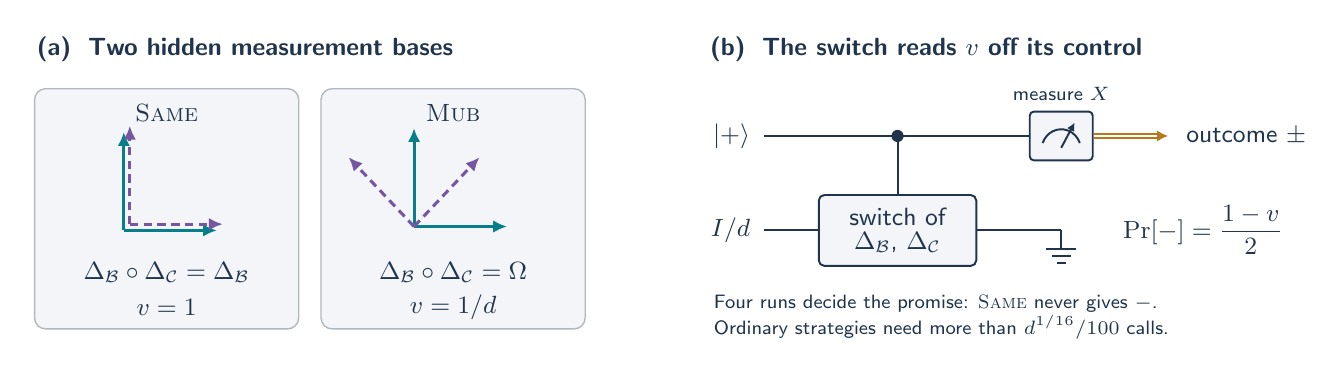
\begin{tikzpicture}[x=.945cm,y=1cm,>=Latex,
 axA/.style={draw=teal,line width=1.1pt,-{Latex[length=5pt,width=4.5pt]}},
 axB/.style={draw=violet,line width=1.1pt,densely dashed,-{Latex[length=5pt,width=4.5pt]}}]
%% (a) the two promises
\node[figtitle] at (-.1,3.55) {(a)\; Two hidden measurement bases};
\draw[figpanel] (0,0) rectangle (3.55,3.05);
\node[figstep,anchor=north] at (1.775,2.98) {\Same};
\draw[axA] (1.2,1.25) -- (2.45,1.25); \draw[axA] (1.2,1.25) -- (1.2,2.5);
\draw[axB] (1.28,1.33) -- (2.53,1.33); \draw[axB] (1.28,1.33) -- (1.28,2.58);
\node[figlab] at (1.775,.72) {$\Delta_{\mathcal B}\circ\Delta_{\mathcal C}=\Delta_{\mathcal B}$};
\node[figlab] at (1.775,.27) {$v=1$};
\draw[figpanel] (3.85,0) rectangle (7.4,3.05);
\node[figstep,anchor=north] at (5.625,2.98) {\Mub};
\draw[axA] (5.1,1.3) -- (6.35,1.3); \draw[axA] (5.1,1.3) -- (5.1,2.55);
\draw[axB] (5.1,1.3) -- (5.98,2.18); \draw[axB] (5.1,1.3) -- (4.22,2.18);
\node[figlab] at (5.625,.72) {$\Delta_{\mathcal B}\circ\Delta_{\mathcal C}=\Omega$};
\node[figlab] at (5.625,.27) {$v=1/d$};
%% (b) the switch readout
\begin{scope}[xshift=8.55cm]
\node[figtitle] at (-.1,3.55) {(b)\; The switch reads $v$ off its control};
\draw[figwire] (.75,2.45) -- (4.75,2.45);
\draw[figwire] (.75,1.25) -- (4.75,1.25);
\node[figlab,anchor=east] at (.7,2.45) {$\ket+$};
\node[figlab,anchor=east] at (.7,1.25) {$I/d$};
\node[draw=navy,fill=mist,rounded corners=2pt,line width=.7pt,minimum width=2.0cm,minimum height=.9cm,font=\small\sffamily,text=navy,align=center] (sw) at (2.55,1.25) {switch of\\[-2pt]$\Delta_{\mathcal B}$, $\Delta_{\mathcal C}$};
\fill[navy] (2.55,2.45) circle (2.2pt); \draw[figwire] (2.55,2.45) -- (sw.north);
\node[gateK,minimum height=.62cm,minimum width=.8cm] (mx) at (4.75,2.45) {};
\draw[figwire] (4.5,2.36) arc (160:20:.266);
\draw[figwire,-{Latex[length=3pt,width=3pt]}] (4.75,2.3) -- (4.93,2.62);
\node[figtiny,anchor=south] at (4.75,2.78) {measure $X$};
\draw[figcc] (mx.east) -- ++(1.0,0);
\node[figlab,anchor=west] at (6.3,2.45) {outcome $\pm$};
\draw[figwire] (4.75,1.25) -- (4.75,1.02); \draw[figwire] (4.55,1.02) -- (4.95,1.02);
\draw[figwire] (4.62,.93) -- (4.88,.93); \draw[figwire] (4.69,.84) -- (4.81,.84);
\node[figlab,anchor=west] at (5.45,1.25) {$\Pr[-]=\dfrac{1-v}{2}$};
\node[figtiny,anchor=north west,align=left] at (-.05,.55) {Four runs decide the promise: \Same{} never gives $-$.\\Ordinary strategies need more than $d^{1/16}/100$ calls.};
\end{scope}
\end{tikzpicture}
\caption{The task of Theorem~\ref{thm:c6}. (a)~Two boxes measure in
hidden bases $\mathcal B$ (solid) and $\mathcal C$ (dashed) and discard
the outcomes. The bases either coincide or are mutually unbiased. In
both cases the two channels commute: the two orders of composition give
the same channel ($\Delta_{\mathcal B}$ under \Same{}, $\Omega$ under
\Mub{}), so comparing the orders reveals nothing. Telling the two
composites apart is possible but, for hidden bases, costly
(Theorem~\ref{thm:c6}). (b)~The switch, with control
$\ket+$ and a maximally mixed target, turns the relation between the
bases into a bias of the control: the outcome $-$ of an $X$ measurement
has probability $(1-v)/2$, where $v$ is the visibility.}
\label{fig:geometry}
\end{figure}

\paragraph{Error $1/2$ with two calls.}
Measure the control in the basis $\{\ket0,\ket1\}$ and apply $B\circ A$
or $A\circ B$ to the target accordingly. This ordinary strategy
implements $\mathcal D\circ\SW[A,B]$, where $\mathcal D$ dephases the
control. Since $\frac12\norm{\id-\mathcal D}_\diamond=\frac12$, its
error is at most $1/2$. Hence
the threshold $\epsilon<1/2$ in Theorem~\ref{thm:simulation-summary}
cannot be raised.

\paragraph{Any error with finitely many calls.}
The deterministic port-based teleportation processor
of~\cite{pirandola2019} consumes $M$ copies
of the Choi state of a channel, each prepared with one call. It applies
the channel to an arbitrary input within diamond-norm distance
$2d(d-1)/M$, that is, with error at most $d(d-1)/M$ in the sense
of~\eqref{eq:simulation-error}. Use it for both boxes. The processors are known operations
on separate program registers, so an ordinary strategy may apply them in
a coherently controlled order. It remains to check
that the switch does not amplify an error made in one box. The switch
with one slot filled by a known channel $B$ is a circuit with one open
slot. Indeed, let $W_B$ be
a unitary dilation of $B$ on the target and an environment. Apply $W_B$
if the control is $\ket1$, call $A$, apply $W_B$ on the same environment
if the control is $\ket0$, and discard the environment. The switch is
therefore contractive in the diamond norm in each slot. Replacing the
two boxes one at a time by their processors gives error at most
$2d(d-1)/M$, with $2M$ calls. Hence the least budget
$Q_{\rm sim}(\epsilon)$ of an ordinary strategy with error at most
$\epsilon$ obeys
\[
 Q_{\rm sim}(\epsilon)
 \le2\left\lceil\frac{2d(d-1)}\epsilon\right\rceil,
 \qquad 0<\epsilon<1.
\]
This construction makes no claim of efficient processing; it bounds the
number of calls only. At fixed error, the number of calls needed for
approximate simulation thus lies between $\Omega(d^{1/4})$ and
$O(d^2)$.

\section{A single number is already hard}\label{sec:c6-proof}

We prove Theorem~\ref{thm:c6}. The task is
shown in \reffig{fig:geometry}. The switch side is a short calculation.
The lower bound has two parts. The first replaces the two hidden
measurement devices by a \emph{label cache}, a simple trace-preserving
process in which the hidden bases enter in one place only. The second
shows that this one place reveals almost nothing, because the labels in
the cache are invariant under a common unknown rotation.

\subsection{The switch reads the number directly}\label{sec:switch-test}

Recall from Section~\ref{sec:visibility} that the experiment with
control $\ket+$, target $I/d$, and an $X$ measurement of the control
gives the outcome minus with probability $(1-v)/2$, and that $v=1$ under
\Same{} and $v=1/d$ under \Mub{} by~\eqref{eq:basis-visibility}. Run
four independent experiments. Declare \Mub{} if any of them gives minus,
and \Same{} otherwise. A \Same{} instance never errs. A \Mub{} instance
is missed with probability $((1+1/d)/2)^4\le(3/4)^4=81/256$. This is the
switch experiment of Gao et al.~\cite{gao2023}, specialized to the two
promises, and it proves the upper bound in Theorem~\ref{thm:c6}.

The same experiment estimates the visibility of any pair of channels.
The mean of $m$ outcomes $\pm1$ has expectation $v(A,B)$. By Hoeffding's
inequality it deviates from $v(A,B)$ by more than $\epsilon$ with
probability at most $2e^{-m\epsilon^2/2}$, which is at most
$2e^{-2}<1/3$ for $m=\lceil4/\epsilon^2\rceil$.

\subsection{A shared hidden orientation defeats ordinary strategies}

\paragraph{The hard instances.}
The lower bound uses one Haar-random unitary $U$, sampled once and
reused at every call. In the two cases the pairs of boxes are
\begin{equation}\label{eq:c6-priors}
 (\Delta_U,\Delta_U)
 \quad\text{and}\quad
 (\Delta_U,\Delta_{UH}),
 \qquad H=H_2^{\otimes n}.
\end{equation}
We call these two distributions over pairs of boxes the two
\emph{priors}. Here $\Delta_U$ dephases in the basis formed by the columns of $U$, and
$H$ is the known Walsh--Hadamard transform. Every sample satisfies its
promise exactly. The shared orientation matters: two independently
chosen random bases would not be mutually unbiased. A strategy that
succeeds with probability $2/3$ on every promised pair succeeds with at
least that probability on average over each prior, so it suffices to
show that few calls cannot tell the two priors apart.


Fix an ordinary strategy with budget $q$, and let $\rho_0,\rho_1$ denote its
final states averaged over the two priors~\eqref{eq:c6-priors}. We use
$\TD(\rho,\sigma)=\norm{\rho-\sigma}_1/2$, also for positive
subnormalized states.

\begin{lemma}[Shared-basis indistinguishability]\label{lem:c6-comparison}
If $q\ge1$ and $4q\le d$, then
\begin{equation}\label{eq:c6-comparison}
\begin{split}
 \TD(\rho_0,\rho_1)\le{}&
 \frac{18(2q)(2q+1)}{d^{1/8}}
 +2E(q,d)+14q\delta_{2q}\\
 &+2B(q,d)+\frac{8q(q-1)}d.
\end{split}
\end{equation}
Here $E(q,d)$, $\delta_t$ and $B(q,d)$ are the errors of forward
deletion, of polar normalization and of fresh births, derived in
Appendix~\ref{sec:c6-recording}:
\begin{gather*}
 E(q,d)=\sum_{i=1}^q\sqrt{\frac{2(2i-1)}{d-2i+2}},\qquad
 \delta_t=\sqrt{\frac{2t(t+1)}d}+\frac td,\\
 B(q,d)=\sum_{i=2}^q\left(\sqrt{\frac{2i-3}{d-i+2}}
       +\sqrt{\frac{2(i-1)}{d-i+1}}\right).
\end{gather*}
In particular, if
$1\le q\le d^{1/16}/100$, the right side is at most $215/10000<1/3$.
\end{lemma}

The functions $E(q,d)$ and $B(q,d)$ are not related to the effect $E$
of Section~\ref{sec:approximation} or to the box $B$. We now carry out
the two parts announced at the start of the section. The comparison of
the two caches explains why quantum memory does not recover the
relation between the bases, and it is proved in full below
(Lemma~\ref{lem:invariant-label} and the paragraph that follows it).
The reduction to the cache justifies applying that explanation to the
actual devices. For it we give a guide here and derive every error term
in Appendix~\ref{sec:c6-recording}. Four structural statements listed
there are given with their reasons only; the Lean formalization
(Appendix~\ref{sec:formal-status}) establishes the lemma and takes none
of them as a hypothesis.

\begin{figure}[t]
\centering
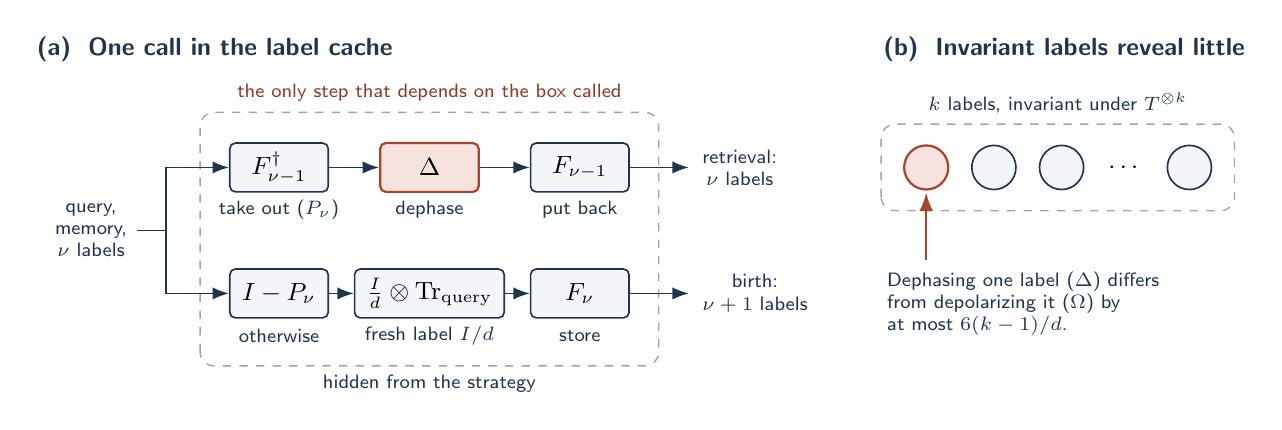
\begin{tikzpicture}[x=.955cm,y=1cm,>=Latex,
 cbox/.style={draw=navy,fill=mist,rounded corners=2pt,line width=.6pt,minimum height=.62cm,minimum width=1.25cm,font=\small,inner sep=2pt},
 hbox/.style={draw=rust,fill=paleRust,rounded corners=2pt,line width=.8pt,minimum height=.62cm,minimum width=1.25cm,font=\small,inner sep=2pt},
 carr/.style={->,draw=navy,line width=.65pt},
 lbl/.style={circle,draw=navy,fill=mist,line width=.6pt,minimum size=.56cm,inner sep=0pt}]
%% (a) one call
\node[figtitle] at (-.1,3.3) {(a)\; One call in the label cache};
\node[figtiny] (in) at (.75,1.0) {query,\\memory,\\$\nu$ labels};
\draw[draw=navy!45,dashed,rounded corners=5pt,line width=.5pt] (2.2,-.72) rectangle (8.3,2.5);
\node[cbox] (dec) at (3.25,1.8) {$F_{\nu-1}^\dagger$};
\node[hbox] (dep) at (5.25,1.8) {$\Delta$};
\node[cbox] (enc) at (7.25,1.8) {$F_{\nu-1}$};
\node[cbox] (prj) at (3.25,.2) {$I-P_\nu$};
\node[cbox,minimum width=1.9cm] (prep) at (5.25,.2) {$\frac Id\otimes\Tr_{\rm query}$};
\node[cbox] (brt) at (7.25,.2) {$F_\nu$};
\node[figtiny,anchor=west] at (8.75,1.8) {retrieval:\\$\nu$ labels};
\node[figtiny,anchor=west] at (8.75,.2) {birth:\\$\nu+1$ labels};
\draw[carr] (in.east) -- (1.75,1.0) |- (dec.west);
\draw[carr] (1.75,1.0) |- (prj.west);
\draw[carr] (dec) -- (dep); \draw[carr] (dep) -- (enc); \draw[carr] (enc) -- (8.7,1.8);
\draw[carr] (prj) -- (prep); \draw[carr] (prep) -- (brt); \draw[carr] (brt) -- (8.7,.2);
\node[figtiny] at (3.25,1.26) {take out ($P_\nu$)}; \node[figtiny] at (5.25,1.26) {dephase}; \node[figtiny] at (7.25,1.26) {put back};
\node[figtiny] at (3.25,-.34) {otherwise}; \node[figtiny] at (5.25,-.34) {fresh label $I/d$}; \node[figtiny] at (7.25,-.34) {store};
\node[figtiny,text=rust!85!black] at (5.25,2.75) {the only step that depends on the box called};
\node[figtiny] at (5.25,-.95) {hidden from the strategy};
%% (b) invariant labels
\begin{scope}[xshift=10.75cm]
\node[figtitle] at (-.1,3.3) {(b)\; Invariant labels reveal little};
\draw[draw=navy!45,dashed,rounded corners=5pt,line width=.5pt] (0,1.25) rectangle (4.7,2.35);
\node[lbl,draw=rust,fill=paleRust,line width=.8pt] (l1) at (.6,1.8) {};
\node[lbl] at (1.5,1.8) {}; \node[lbl] at (2.4,1.8) {}; \node[lbl] at (4.1,1.8) {};
\node[font=\small] at (3.25,1.8) {$\cdots$};
\node[figtiny] at (2.35,2.62) {$k$ labels, invariant under $T^{\otimes k}$};
\draw[draw=rust,line width=.8pt,->] (.6,.62) -- (.6,1.48);
\node[figtiny,anchor=north west,align=left] at (-.05,.6) {Dephasing one label ($\Delta$) differs\\from depolarizing it ($\Omega$) by\\at most $6(k-1)/d$.};
\end{scope}
\end{tikzpicture}
\caption{The mechanism behind the lower bound of Theorem~\ref{thm:c6}.
(a)~One call in the label cache, whose hidden state is a list of $\nu$
labels with their images. With effect $P_\nu$ a stored label is retrieved: it is taken
out, dephased with the dephaser $\Delta$ of the box that was called, and
put back. With the complementary effect $I-P_\nu$ a label is born: the
query is discarded and a maximally mixed label is stored. The hidden bases enter only in the highlighted step. (b)~The stored labels are invariant under a
common rotation $T$. Dephasing one of $k$ such labels in any basis is
within $6(k-1)/d$ of depolarizing it (Lemma~\ref{lem:invariant-label}),
so the two promises give nearly the same final state.}
\label{fig:cache}
\end{figure}

\paragraph{From shared Haar access to a label cache.}
The first part of the proof is a chain of five replacements, listed with
their costs in Table~\ref{tab:hybrids} of
Appendix~\ref{sec:c6-recording}. We say here what each of them does.

A call to $\Delta_U$ or to $\Delta_{UH}$ can be written as $U^\dagger$,
followed by a known dephasing in the computational or in the Hadamard
basis, followed by $U$. The choice of the box affects only the middle
operation. A strategy with $q$ calls is therefore an experiment with
$2q$ alternating inverse and forward queries to one Haar-random unitary.
The inverse queries belong to this description of the devices; the
strategy itself is not given access to $U^\dagger$.

The first replacement is the path-recording theorem of Ma and
Huang~\cite{mahuang2025}. It replaces the Haar unitary by a
\emph{recording process}, which does not apply any fixed unitary.
Instead it keeps hidden lists of input--output pairs, and answers a
query either by undoing a recorded pair or by recording a new one.
For $2q$ queries the replacement costs $9(2q)(2q+1)d^{-1/8}$ in trace
distance, for each prior. We call the first entry of a stored pair
a \emph{label} and the second its \emph{image}.

Four further replacements simplify the recording process. A forward
query may add a pair to the lists or remove one. Because the query has
just been dephased, removal is unlikely, and replacing every forward
step by the creation of a new pair (forward deletion) costs $E(q,d)$. The creation
operators are then replaced by the polar isometries of the bosonic
creation operators, which are exactly covariant under a common rotation
of the labels (polar normalization); this costs $7q\delta_{2q}$. An inverse query either
\emph{retrieves} a stored label or gives \emph{birth} to a new one.
Restricting births to labels orthogonal to all earlier measurement
outcomes, and dropping the part of a retrieval that overlaps an earlier
birth (fresh births), costs $B(q,d)$. After this restriction
the lists record permanently which of the two happened, so that the two
alternatives never interfere again. Finally the birth isometry is replaced by its unnormalized form, and
the weights with which labels are born are made uniform; the two
changes cost $q(q-1)/d$ together. The images recorded at births, which
no later step uses, can then be traced out exactly, although they are
entangled with the memory of the strategy.

What remains is a trace-preserving process on one list, the
\emph{label cache} of \reffig{fig:cache}(a). Its hidden state consists
of a number $\nu$ of stored labels, with $0\le\nu\le q$, and of the
labels themselves. Each stored label keeps its image, which stays
hidden and plays no role below except as part of the reference system
in Lemma~\ref{lem:invariant-label}. A call is made only when $\nu<q$, and at $\nu=q$ the
process is extended by the identity. Let $F_\nu$ be the isometry that
stores the content of the query system as a new label, taking $\nu$
labels to $\nu+1$. Put $P_\nu=F_{\nu-1}F_{\nu-1}^\dagger$ for
$\nu\ge1$, and $P_0=0$. A call to a box with dephasing channel $\Delta$, its \emph{dephaser}
for short, acts as the sum of the two maps
\begin{equation}\label{eq:c6-cache}
\begin{aligned}
 \mathcal R_{\Delta,\nu}(X)
 &=F_{\nu-1}(\Delta\otimes\id)
       (F_{\nu-1}^\dagger XF_{\nu-1})F_{\nu-1}^\dagger,\\
 \mathcal B_\nu(X)
 &=F_\nu\left[\frac Id\otimes\Tr_{\rm query}
       ((I-P_\nu)X(I-P_\nu))\right]F_\nu^\dagger.
\end{aligned}
\end{equation}
The \emph{retrieval} $\mathcal R_{\Delta,\nu}$ takes a stored label out
into the query system, dephases it with the dephaser of the box that was
called, and puts it back. The number of labels stays $\nu$, and the
retrieval is zero at $\nu=0$. The \emph{birth} $\mathcal B_\nu$ discards
the query, stores a maximally mixed label, and raises the number of
labels to $\nu+1$. The two branches occur with the complementary effects
$P_\nu$ and $I-P_\nu$, so the process is trace preserving on all states.
The memory of the strategy is not touched. The hidden bases enter in one
place only: the dephaser $\Delta$ applied to a retrieved label.

\paragraph{The information in an invariant label.}
The second part of the proof rests on the following estimate, shown in
\reffig{fig:cache}(b). It concerns a state of $k$ labels and a reference
system $Z$; the state is assumed not to change when all $k$ labels are
rotated by the same unitary. The reference $Z$ holds everything else:
the images of the stored labels, the memory of the strategy, with
arbitrary entanglement, and any other side information. In the lemma,
$X$ is an arbitrary positive operator and $T$ an arbitrary unitary. The
lemma applies to the cache because the list of $k$ pairs of a label and
an image embeds isometrically in the tensor product of $k$ labels and
$k$ images, and a common rotation of the labels preserves the embedded
subspace.

\begin{lemma}[Dephasing invariant labels]\label{lem:invariant-label}
Let $X\succeq0$ have trace $s$ on $k\ge1$ labels of dimension $d\ge2$ and
a reference $Z$. Suppose $X$ is invariant under $T^{\otimes k}\otimes I_Z$
for every unitary $T$. For any rank-one dephaser $\Delta$ on the first label,
\begin{equation}\label{eq:invariant-label}
 \norm{(\Delta\otimes\id)(X)-(\Omega\otimes\id)(X)}_1
 \le\frac{6(k-1)}d\,s.
\end{equation}
\end{lemma}
\begin{proof}
Take $s=1$ and let $\Delta$ dephase in the computational basis; the
invariance of $X$ then gives the bound for every other basis, and
homogeneity restores $s$. The first label has marginal $I/d$. Let
$\sigma_j=d\bra jX\ket j$ be the state of the other $k-1$ labels and of
$Z$, given that the first label has the value $j$, and let
$\bar\sigma=d^{-1}\sum_j\sigma_j$. Then
\[
 (\Delta\otimes\id)(X)=\frac1d\sum_j\proj j\otimes\sigma_j,
 \qquad
 (\Omega\otimes\id)(X)=\frac Id\otimes\bar\sigma .
\]
The blocks of the difference are orthogonal, so their trace norms add,
and the left side of~\eqref{eq:invariant-label} equals
$d^{-1}\sum_j\norm{\sigma_j-\bar\sigma}_1$. It therefore suffices to
bound $\norm{\sigma_j-\bar\sigma}_1$ for each $j$.

For $j\ne a$, let $P_{ja}$ be the projector onto the subspace in which
none of the remaining $k-1$ labels has the value $j$ or $a$. The unitary
that exchanges $\ket j$ and $\ket a$ acts as the identity on this
subspace, and $X$ is invariant under it, so
$P_{ja}\sigma_jP_{ja}=P_{ja}\sigma_aP_{ja}$. Invariance under diagonal
unitaries implies that $\sigma_j$ commutes with the operators that count
how many of the remaining labels have each basis value, and hence with
$P_{ja}$. The states $\sigma_j$ and $\sigma_a$ are thus positive,
commute with $P_{ja}$, and agree after compression by $P_{ja}$. Hence
\[
 \norm{\sigma_j-\sigma_a}_1
 \le\Tr((I-P_{ja})\sigma_j)+\Tr((I-P_{ja})\sigma_a),
\]
and no off-diagonal block is neglected in this step.

It remains to bound the two traces. Fix one of the remaining labels.
Its joint marginal with the first label is invariant under $T\otimes T$
for every unitary $T$, and the projector onto equal values of the two
labels twirls to $(I+\operatorname{SWAP})/(d+1)$. Given that the first
label has the value $j$, the other label therefore has the same value
$j$ with probability at most $2/(d+1)$. It has a given different value
$a$ with probability at most $1/(d-1)$. A union bound over the $k-1$
remaining labels gives
\[
 \Tr((I-P_{ja})\sigma_j)
 \le(k-1)\left(\frac2{d+1}+\frac1{d-1}\right),
\]
and likewise for $\sigma_a$. Averaging the bound on
$\norm{\sigma_j-\sigma_a}_1$ over $a$, where the term $a=j$ vanishes,
gives
\[
 \norm{\sigma_j-\bar\sigma}_1
 \le\frac{2(k-1)(3d-1)}{d(d+1)}\le\frac{6(k-1)}d.
\]
This proves~\eqref{eq:invariant-label}. The reference $Z$ is carried
along unchanged throughout.
\end{proof}

\paragraph{Comparing the two caches.}
Replace the dephaser $\Delta$ in every retrieval
of~\eqref{eq:c6-cache} by the depolarizing channel $\Omega$. The
resulting \emph{reference cache} does not depend on the hidden bases, so
it is the same for both priors. At every time and for every number
$\nu$ of labels, its state is invariant under a common rotation of all
stored labels. This follows by induction over the calls. Initially
there are no labels. The known operations of the strategy act on the
query and the memory only. The isometries $F_\nu$ are covariant under a
common rotation of the labels (Appendix~\ref{sec:c6-A2}). A birth
stores $I/d$, and a reference retrieval depolarizes the label that it
takes out. The invariance holds with arbitrary correlations with the
memory and for any classical choice of the box.

Now compare the cache of either prior with the reference cache, one
retrieval at a time. Run the reference cache up to a given call and the
actual cache from that call on. In a retrieval at that call, the
isometry $F_{\nu-1}^\dagger$ turns the $\nu$ stored labels into the
label that is taken out and $\nu-1$ remaining labels. These $\nu\le q$
labels are invariant, so by Lemma~\ref{lem:invariant-label}, with all
other systems in $Z$, replacing $\Delta$ by $\Omega$ changes the state
by at most $6(q-1)/d$ times its trace, in trace norm. The later steps
are trace preserving and do not increase this difference. Summing over
the $q$ calls, each cache differs from the reference by at most
$3q(q-1)/d$ in trace distance, and the two caches differ from each
other by at most $6q(q-1)/d$. Adding the costs of the five replacements
of Table~\ref{tab:hybrids}, which are paid once for each prior, proves
Lemma~\ref{lem:c6-comparison}.

\paragraph{Concluding the lower bound.}
If $1\le q\le d^{1/16}/100$, then $4q\le d$.
Lemma~\ref{lem:c6-comparison} gives $\TD(\rho_0,\rho_1)<1/3$, so the
best equal-prior success probability $(1+\TD)/2$ is less than $2/3$.
Worst-case success $2/3$ would imply the same average success on these
priors, a contradiction. A strategy with no calls cannot distinguish the
priors. This proves the lower bound for every $n\ge1$, including the
dimensions with $d^{1/16}/100<1$, for which the theorem asserts only
that at least one call is needed.


\subsection{Estimating and testing the visibility}\label{sec:robust}

\begin{proof}[Proof of Theorem~\ref{thm:c6}\textup{(b)}]
Under \Same{} the visibility is $1$, and under \Mub{} it is
$1/d\le1/2$. An estimate within $\epsilon<1/4$ of the true value is
above $3/4$ in the first case and below $3/4$ in the second. Comparing
the estimate with $3/4$ therefore decides the promise with the same
calls and the same success probability, and part~(a) gives
the lower bound. Section~\ref{sec:switch-test} gave the upper bound.
\end{proof}

\begin{remark}[The separation is asymptotic]\label{rem:crossover}
The quantity $d^{1/16}/100=2^{n/16}/100$ reaches $1$ at $n=107$ qubits,
and it exceeds the eight calls made by the four-switch test only for
$n\ge155$. For smaller $n$ Theorem~\ref{thm:c6} is true but does not
separate the two kinds of access. Neither the constant nor the exponent
is optimized: the exponent $1/16$ is inherited from the error $d^{-1/8}$
of the recording theorem that the proof imports. In the other
direction, simulate each of the four switch uses to error $1/250$ with
the processor of Section~\ref{sec:simulation}. The total error of the
test stays below $1/3$, so $O(d^2)$ calls of an ordinary strategy
suffice. The same holds for estimating $v$ to a fixed accuracy on
arbitrary pairs. For a related promise, an advantage of the switch at
$d=4$ is certified exactly in Proposition~\ref{prop:two-call}.
\end{remark}

\begin{remark}[A possible direct test]\label{rem:direct-test}
For the promise problem alone we expect a direct test to need fewer
calls. The following is a sketch, not a proof. Apply
both boxes in turn to copies of a known Haar-random pure state $\psi$.
Under \Mub{} the output is exactly $I/d$. Under \Same{} it is
$\Delta_{\mathcal B}(\psi)$, whose trace distance from $I/d$ has mean
$(1-1/d)^d\ge1/4$ and concentrates around it by L\'evy's lemma. Testing
a state against the maximally mixed state at constant trace distance
takes a number of copies of order $d$~\cite{odonnell2015}. It suggests
that $O(d)$ calls suffice, so that the exponent for the promise problem
would lie between $1/16$ and $1$.
\end{remark}

For arbitrary channels, the decision problem has a version with a
constant gap in the visibility.


\begin{corollary}[Constant-gap interference testing]\label{thm:testing}
Let $d=2^n$, $n\ge1$. Every ordinary strategy that, for every pair of
channels $A,B$ on $\C^d$ with $v(A,B)\ge2/3$ or $v(A,B)\le1/3$, decides
which of the two holds with probability at least $2/3$ has budget
greater than $d^{1/16}/100$. Eighty uses of the switch, with 160 calls in
total, suffice. For $n\ge2$ the lower bound holds even when both boxes
are rank-one dephasing channels.
\end{corollary}
\begin{proof}
For $n\ge2$, \textnormal{\textsc{Same}} and \textnormal{\textsc{Mub}} have visibilities $1$ and
$1/d\le1/4$, so Theorem~\ref{thm:c6} gives the lower bound. At $n=1$ we have $d^{1/16}/100<1$, so the claim is that at least one
call is needed; a strategy with no calls cannot distinguish two equal
dephasing channels ($v=1$) from two completely depolarizing channels
($v=1/4$). For the upper bound, the switch experiment gives the outcome
$+$ with probability $(1+v)/2$, which is at least $5/6$ in the first
case and at most $2/3$ in the second. Thresholding its empirical frequency at $3/4$,
that is, declaring high visibility when at least $60$ of $80$ outcomes are
plus, leaves margin $1/12$. By Hoeffding's inequality this test, which uses
the estimator of~\cite{gao2023}, errs with probability at most
$e^{-m/72}<1/3$ for $m=80$.
\end{proof}


\subsection{The number at work: validating a noise model}\label{sec:validation}

Theorem~\ref{thm:c6} concerns two measurement devices. The same number
is informative about a single noisy device, and its hardness carries
over. The statements of this subsection are proved here or in the
supplementary material; they are not part of the Lean formalization.

\paragraph{A certificate of model mismatch.}
Let a device apply the same unknown channel $\mathcal E$ on $\C^d$ at
every use, and let a known channel $\mathcal M$ be a model of it. Put
the device in both slots of the switch and write
$v(\mathcal E)=v(\mathcal E,\mathcal E)$ for the resulting
\emph{self-visibility}. Since
$1-v(A,B)=\frac1{2d}\sum_{i,j}\norm{A_iB_j-B_jA_i}_2^2$, the
self-visibility equals $1$ exactly when the Kraus operators of
$\mathcal E$ commute with one another. It is $1$ for every unitary
channel and for dephasing in any one basis, and it is $1/d^2$ for the
completely depolarizing channel $\Omega$.

\begin{proposition}[Model mismatch]\label{prop:mismatch}
For all channels $\mathcal E,\mathcal M$ on $\C^d$,
\[
 \frac12\norm{\mathcal E-\mathcal M}_\diamond
 \ge\frac14\,\bigl\lvert v(\mathcal E)-v(\mathcal M)\bigr\rvert .
\]
\end{proposition}
\begin{proof}
The switch is linear in each slot, so
$\SW[\mathcal E,\mathcal E]-\SW[\mathcal M,\mathcal M]
=\SW[\mathcal E-\mathcal M,\mathcal E]+\SW[\mathcal M,\mathcal E-\mathcal M]$.
It is contractive in the diamond norm in each slot
(Section~\ref{sec:simulation}), so the left side has diamond norm at
most $2\norm{\mathcal E-\mathcal M}_\diamond$. The visibility is the
expectation of the observable $X$ of the control in the output of the
switch on a fixed input, and expectations of $X$ in two states differ
by at most the trace norm of their difference.
\end{proof}

A measured self-visibility that differs from the prediction of the
model by more than the statistical error therefore proves that the
model is wrong, by a stated amount in the diamond norm. The certificate
is one-sided: agreement proves nothing, since all unitary channels have
self-visibility $1$.

\paragraph{Two kinds of noise with the same fidelity.}
Fix a strength $0<p\le1$ and a hidden unitary $U$, and consider the two
channels
\begin{equation}\label{eq:validation-pair}
 \mathcal E_{p,U}=(1-p)\id+p\,\Delta_U,
 \qquad
 \mathcal M_p=(1-p)\id+p\,\Lambda,
 \qquad
 \Lambda=\frac{\id+d\,\Omega}{d+1}.
\end{equation}
The channel $\mathcal E_{p,U}$ is noise with a preferred basis: with
probability $p$ it dephases in the basis given by $U$, the same basis at
every use. The channel $\mathcal M_p$ is a depolarizing channel, the
model with no preferred basis. It is the average of the first channel
over the basis, $\mathcal M_p=\E_U\mathcal E_{p,U}$. Three standard
diagnostics see little or no difference between the two: the fidelity,
the statistics of any single use, and the unitarity. Their
entanglement fidelities are equal, $1-p+p/d$ for every $U$, and so are
their average gate fidelities, which are a function of the entanglement
fidelity. Any experiment that uses the device once has the same
statistics for $\mathcal M_p$ as on average over $U$ for
$\mathcal E_{p,U}$. And the unitarities~\cite{wallman2015} of the two
channels differ by $p^2d/(d+1)^2$, which vanishes as $d$ grows. Yet the
channels are far apart: on half of a maximally entangled state their
outputs have trace distance $p(d-1)/(d+1)$. The self-visibility
separates them by an amount that does not depend on $d$:
\begin{equation}\label{eq:validation-visibility}
 v(\mathcal E_{p,U})=1,
 \qquad
 v(\mathcal M_p)=1-p^2\,\frac{d-1}{d+1}.
\end{equation}
The first value holds because the Kraus operators $\sqrt{1-p}\,I$ and
$\sqrt p\,U\proj jU^\dagger$ commute. For the second, write
$\mathcal M_p=\alpha\id+(1-\alpha)\Omega$ with $\alpha=1-pd/(d+1)$. The
visibility is bilinear, $v(\id,B)=1$ for every channel $B$, and
$v(\Omega)=1/d^2$, so
$v(\mathcal M_p)=1-(1-\alpha)^2(1-d^{-2})$.

\begin{corollary}[Validating a noise model]\label{cor:validation}
Let $d=2^n$, $n\ge1$, and $0<p\le1$. A device applies the same channel
at every use, promised to be either the model $\mathcal M_p$ or
$\mathcal E_{p,U}$ for an unknown $U$.
\begin{enumerate}
\item[\textup{(a)}] Every ordinary strategy that decides which holds
with success probability at least $2/3$, for $\mathcal M_p$ and for
every $U$, has budget greater than $d^{1/16}/(1400\,p)$.
\item[\textup{(b)}] Seven uses of the switch suffice, with
$k=\lceil3/(2p)\rceil$ consecutive uses of the device in each slot.
They make $14k=O(1/p)$ calls and have one-sided error less than $1/3$.
\end{enumerate}
\end{corollary}

\begin{proof}
(b) The channel in each slot is the $k$th power of the device. For
$\mathcal E_{p,U}$ this power is again a mixture of the identity and
$\Delta_U$, so its Kraus operators commute and the outcome minus never
occurs. For the model the power is $\alpha^k\id+(1-\alpha^k)\Omega$,
and the outcome minus has probability
$\frac12(1-\alpha^k)^2(1-d^{-2})$. Since $k\ge(d+1)/(pd)$, we have
$\alpha^k\le e^{-1}$, and this probability is at least
$\frac38(1-e^{-1})^2>0.149$. Declare the model if any of seven
independent uses gives minus. The error is zero for $\mathcal E_{p,U}$
and at most $0.851^7<1/3$ for the model.

(a) Let $L=\lfloor d^{1/16}/200\rfloor$. Consider first a \emph{strong}
device, which applies $\Delta_U$ with Haar-random $U$ or applies
$\Lambda$, and an ordinary strategy that uses it at most $L$ times. We
claim that the strategy decides between the two cases with probability
at most $2053/4000$. For $L=0$ this is trivial. For $L\ge1$, replace
each use by a call to $A$ followed by a call to $B$.
Under the two priors~\eqref{eq:c6-priors} the composition $B\circ A$ is
$\Delta_U$ and $\Delta_{UH}\circ\Delta_U=\Omega$, respectively, so
Lemma~\ref{lem:c6-comparison} with budget $2L\le d^{1/16}/100$ bounds
the distance between the final states for $\Delta_U$, averaged over
$U$, and for $\Omega$ by $215/10000$. Moreover
$\frac12\norm{\Lambda-\Omega}_\diamond\le1/(d+1)$, and $L$ uses add at
most $L/(d+1)\le1/200$. The final states for $\Delta_U$ and for
$\Lambda$ are therefore within $53/2000$, which proves the claim.

Now let an ordinary strategy with budget $Q$ succeed with probability
$2/3$ on $\mathcal M_p$ and on every $\mathcal E_{p,U}$, hence also when $U$ is
Haar-random and the two cases are equally likely. Run it on the strong
device as follows: at each use toss a private coin, and with probability
$p$ use the strong device, otherwise do nothing. This reproduces
$\mathcal E_{p,U}$ and $\mathcal M_p$ exactly. The number of strong uses
has mean at most $pQ$. Stop the strategy when it asks for a strong use
beyond the $L$th; by Markov's inequality this happens with probability
at most $pQ/(L+1)$ in either case, so stopping lowers the success
probability by at most that amount. The stopped strategy, private coins
included, is an ordinary strategy that uses the strong device at most
$L$ times, and therefore
\[
 \frac23-\frac{pQ}{L+1}\le\frac{2053}{4000},
 \qquad\text{that is,}\qquad
 pQ\ge\frac{1841}{12000}\,(L+1)>\frac{d^{1/16}}{1400}. \qedhere
\]
\end{proof}

The dependence on $p$ is optimal for the switch: every use of the device
changes the output of any strategy, with or without the switch, by at
most $\frac12\norm{\mathcal E_{p,U}-\mathcal M_p}_\diamond\le p$, so
success probability $2/3$ needs at least $1/(3p)$ uses. With one use of
the device in each slot the test of part~(b) needs of order $1/p^2$
uses. Part~(b) assumes that one use of the switch orders two blocks of $k$
uses of the device coherently. As in Remark~\ref{rem:crossover}, the
constants in part~(a) are far from tight: the bound exceeds $1/(3p)$
only for $n\ge142$, and it exceeds $21/p$, which the switch test of
part~(b) needs at least, only for $n\ge238$. At $p=3/4$ the two kinds of noise also differ in
their quantum capacity, which is the subject of
Appendix~\ref{sec:capacity-qualification}.

\paragraph{A small exact instance.}
For small systems the advantage can be certified exactly, without the
recording argument.

\begin{proposition}[Two uses, two qubits]\label{prop:two-call}
Let $d=4$. A device applies $\Delta_U$ with Haar-random $U$ or applies
$\Lambda$, each with probability $1/2$. Every ordinary strategy that
uses the device at most twice identifies the case with probability at most
$29/50$. One use of the switch, with the device in both slots,
identifies it with probability $13/20$.
\end{proposition}
\begin{proof}
For the switch, guess $\Lambda$ on the outcome minus, which has
probability $0$ for $\Delta_U$ and $(1-v(\Lambda))/2=3/10$ for
$\Lambda$. For ordinary strategies, the two uses see one of the two
operators $W_0=\E_UJ(\Delta_U)^{\otimes2}$ and
$W_1=J(\Lambda)^{\otimes2}$, where $J$ denotes the unnormalized Choi
operator. A strategy with two uses is a two-slot
tester~\cite{chiribella2008memory}, and its success probability is
$\frac12+\frac12\Tr[(W_0-W_1)T_0]$ for the tester element $T_0$ of the
first guess. The dual of this semidefinite program asks for an operator
$Z\succeq0$ with $Z\succeq W_0-W_1$ whose partial trace over the last
output is $Y\otimes I$, with $I$ on the second input, and with the
partial trace of $Y$ over the first output equal to $\lambda I$ on the
first input; every such $Z$ gives the bound
$\frac12+\frac\lambda2$. The supplementary material contains a rational
matrix $Z$ with $\lambda=4/25$ and a program that constructs $W_0$ from
the Haar moments and verifies the four conditions in exact rational
arithmetic.
\end{proof}

For noise of strength $p$, with $U$ Haar-random and the two cases
equally likely, the same certificate scaled by $p^2$ shows
that two ordinary uses succeed with probability at most
$\frac12+\frac{2}{25}p^2$, whereas the switch attains
$\frac12+\frac{3}{20}p^2$. The bound $29/50$ is not claimed to be
optimal, and the proposition says nothing about more than two uses.

\paragraph{Where the hardness ends.}
Corollary~\ref{cor:validation} needs a basis that is hidden, global and
generic. Three
observations mark the boundary. The first two grant the ordinary
strategy only known operations and the same access to the device; the
third changes the access.
First, suppose that the basis is known to come from a list of $K$
bases. One use of the device on half of a maximally entangled state
gives a copy of its Choi state. After the component along the maximally
entangled state is projected out, the state for $\mathcal E_{p,U}$ is
supported on a $(d-1)$-dimensional subspace determined by the basis,
whereas the state for the model has weight $1/(d+1)$ on each such
subspace. Quantum threshold search~\cite{badescu2024} finds a subspace
of the list that carries the state, if there is one, from
$O(\log^2(K+1))$ copies, and a check of the subspace that it returns
rejects the model. Each copy costs at most $2/p$ uses on average, so
$O(\log^2(K+1)/p)$ uses of the device suffice in total. A basis with a short description is thus not hard in the
number of uses, although the search may take a long time. Second,
suppose that the noise acts on each qubit separately: it dephases
qubit $j$ about its own unknown axis, and the model depolarizes each
qubit with the same fidelity. Take two copies of the Choi state of $k$
consecutive uses. On each qubit, project both copies onto the
complement of the maximally entangled state of that qubit and its
reference, and test the two three-dimensional systems that result for
antisymmetry under exchange. The test never fires for the dephasing noise,
and three repetitions of it miss the model with probability no larger
than that of one use of the switch with the same $k$ in each slot.
Third, if the randomness of the noise can be replayed, so that the same
unitary realization can be applied again, the three-call circuit of
Remark~\ref{rem:unitary} applies to each realization and reproduces the
switch on average. Section~\ref{sec:where} returns to the question of
which devices escape all three observations.

\section{Discussion and open problems}\label{sec:discussion}

\subsection{Where do such black boxes arise?}\label{sec:where}

The three theorems are statements about queries. They show that, for boxes of a particular kind, the switch is worth
exponentially many ordinary calls, or more calls than any bound allows. The main question that they leave open
is whether a computational task of independent interest contains boxes
of that kind.

The proofs and the known counterexamples suggest five properties that
such a box should have.
\begin{enumerate}
\item \emph{Irreversible.} For unitary boxes three calls simulate the
switch.
\item \emph{Record unavailable.} If the outcomes of the two measurements
in Theorem~\ref{thm:c6} are reported, a short ordinary experiment
reproduces the statistics of the switch~\cite{gao2023}.
\item \emph{Generic.} The lower bound uses a Haar-random basis in
dimension $2^n$, and the two structured cases that we checked are easy.
If the strategy can prepare copies of even one vector of the hidden
basis, four swap tests, each after a single call to the other box,
decide the promise with the error of the switch test. If the bases are
known to be stabilizer bases, the boxes are mixtures of Pauli operators,
and calls on halves of maximally entangled states reveal them with a
number of calls of order $n$. Section~\ref{sec:validation} adds two
cases: a basis from a short list, and noise that acts on each qubit
separately.
\item \emph{Persistent.} The same unknown channel is met at every call.
\item \emph{Switchable.} The two orders act on the same instance of the
box, including its environment, so that they share the internal record
of each call. We expect this requirement to be the hardest to meet
physically.
\end{enumerate}

Noise is the operation in a quantum computer that most plainly has the
first two properties, and Section~\ref{sec:validation} works out what
the visibility gives for it. With a noisy device in both slots, the
switch measures how far the Kraus operators of the noise are from
commuting. This certifies a mismatch with a noise model
(Proposition~\ref{prop:mismatch}). It also separates noise that
dephases in a persistent hidden basis from depolarizing noise of the
same fidelity with $O(1/p)$ uses, where an ordinary strategy needs a
number of uses exponential in $n$ (Corollary~\ref{cor:validation}). At
strength $p=3/4$ and for $n\ge4$ the two kinds of noise differ in what
they allow: the first has positive quantum capacity and the second has
none, and any code that works for the first without knowledge of the
basis must have length exponential in $n$
(Appendix~\ref{sec:capacity-qualification}). We regard this as a
candidate and not as an application, for three reasons. Its proof is
not part of the Lean formalization. The hidden basis is generic,
whereas slowly varying noise in hardware is usually low-dimensional or
has Pauli structure; Section~\ref{sec:validation} shows that a basis
with a short description, or noise that acts qubit by qubit, leaves
ordinary strategies with an easy task. And the coherent action of the
switch on the noise is assumed and not derived from a physical model of
the device.

A second candidate is dephasing in the eigenbasis of a Hamiltonian. Let
$H(\lambda)=H_0+\lambda V$ have a nondegenerate spectrum with
eigenvalues $E_i$ at $\lambda=0$, and let $V_{ji}$ be the matrix
elements of $V$ in the eigenbasis of $H_0$. The visibility of the
eigenbasis dephasers of $H(0)$ and $H(\lambda)$ obeys
\[
 1-v=2\lambda^2\chi+O(\lambda^3),
 \qquad
 \chi=\frac1d\sum_{i\ne j}\frac{\lvert V_{ji}\rvert^2}{(E_i-E_j)^2},
\]
by first-order perturbation theory. The quantity $\chi$ is the average
fidelity susceptibility of the eigenstates, a sensitive probe of
quantum chaos~\cite{pandey2020}. Such a dephaser arises when the system
evolves for a random time. But a time average that removes the
coherence between every pair of levels needs a mean evolution time of
at least the order of the inverse of the smallest level spacing, which
is exponential in $n$ for a spectrum of polynomial width; and if the
evolution time is chosen by the experimenter, each realization is a
unitary that can be applied again, and three calls suffice
(Remark~\ref{rem:unitary}). This is an interpretation of the number, and not
yet a task with an advantage.

Other settings share some of the properties. Dissipative primitives and
resets are irreversible and persistent. Error correction without
measurement never produces a classical syndrome, but its checks are
binary measurements in a known Pauli frame, which is far from generic. Commutators govern the error of product formulas, and estimating them
is a natural task; but there the operations are unitary, so the switch
saves a constant factor at most. The difficulty is that persistence invites learning: every natural
family that we know is either structured enough to be learned with
polynomially many calls, or not persistent. We therefore ask:

\begin{quote}
\emph{Is there a natural computational task whose black boxes are
irreversible, generic, persistent and switchable, and keep their
internal record unavailable, so that the exponential query separation
proved here becomes a saving for that task?}
\end{quote}

\subsection{Further open problems}\label{sec:open}

\paragraph{Optimal exponents.}
For approximate simulation at fixed error our bounds place the number
of ordinary calls between $d^{1/4}$ and $d^2$; concurrent work raises
the lower exponent to $1/3$ (Section~\ref{sec:concurrent}). For estimating the visibility it lies between
$d^{1/16}$ and $d^2$, and for the promise problem of
Theorem~\ref{thm:c6} the upper end is probably $d$
(Remark~\ref{rem:direct-test}). Our proof of
Theorem~\ref{thm:simulation-summary} cannot give more than $d^{1/4}$,
because the coherence penalty already limits the number of hidden
unitaries to about $\sqrt d$. The exponent $1/16$ is tied to the error
of the recording theorem with inverse queries. We do not know the true
exponents.

\paragraph{Between unitaries and channels.}
For unitary boxes the switch costs three calls, and for mixtures of
about $\sqrt d$ unitaries it costs $\Omega(d^{1/4})$. It would be
natural to determine how the cost of simulation depends on a measure of
irreversibility, such as the Kraus rank, and in particular what it is
for weakly noisy unitary gates.

\paragraph{Expected cost and postselection.}
Our theorems count calls on the worst run and require success without
conditioning. Two questions are open. Does an exact simulation exist that stops with
probability one without a bound on its number of calls, in particular
one with a finite \emph{expected} number of calls? And how does the
best success probability of a heralded exact simulation depend on the
budget?
Probabilistic simulation was studied in~\cite{bavaresco2025}.

\paragraph{Other processes and other access.}
The switch is the simplest process with indefinite causal order. It
would be interesting to know whether the visibility separation grows for
switches of more than two channels, and whether more general processes
do better than the switch on a learning task. A related axis is access
to a dilation of a channel, which is at least as strong as access to the
switch and has recently been separated from channel
access~\cite{goldin2026,arihara2026}.

\paragraph{Efficient and physically motivated boxes.}
Under a cryptographic assumption, Theorem~\ref{thm:c6} has a version for
boxes with efficient implementations and polynomial-time strategies
(Appendix~\ref{sec:connections}). An unconditional lower bound for a
family of boxes with a natural physical origin would bear
directly on the open question raised in Section~\ref{sec:where}.

\subsection{Concurrent and independent work}\label{sec:concurrent}

The results of this paper were obtained in September 2026. The proofs,
the Lean formalization and the certificates are kept in a
repository~\cite{repo}. Its first commit, of 11 October 2026, already
contains the three theorems with their proofs and the formalization,
whose kernel audit is dated 3 October 2026. While preparing the
manuscript we learned of two preprints, by Cheng~\cite{cheng2026} and by
Goldin~\cite{goldin2026}. Our work is independent of both.

Cheng~\cite{cheng2026} proves that no bounded number of calls gives an
exact simulation of the switch, and treats switches of more than two
channels. Goldin~\cite{goldin2026}, in a study of dilations of
channels, proves that approximate simulation to any fixed error below $1/2$
needs $\Omega(d^{1/3})$ calls, a larger exponent than ours, and gives a
one-bit task that one use of the switch decides.

The proofs have steps in common with ours and are not the same. For
exact simulation, both arguments use mixtures of channels to reduce to
one call to each box, and then treat qubits; ours ends in the exact
certificate of Lemma~\ref{lem:exact-obstruction}, holds for a fixed
control input, and is formalized in Lean. For approximate simulation,
both arguments hide an index that few calls do not repeat; ours bounds
the coherence between the two orders
(Corollary~\ref{cor:coherence}) and gives an explicit trade-off for
mixtures of unitaries. The contents also differ. Neither preprint
considers the visibility of~\cite{gao2023}, measurement devices, or
dephasing in a hidden basis, from which Theorem~\ref{thm:c6} and
Section~\ref{sec:c6-proof} start. The closest statement is the one-bit
task of~\cite{goldin2026}, which one use of the switch decides without
error and for which ordinary strategies need $\Omega(d^{1/3})$ calls.
It differs in the promise and in the number read: one channel from a
specific family occupies both slots, and the control is read for a
known pure target state.

\appendix

\section{From the recording process to the label cache}\label{sec:c6-recording}

This appendix supplies the quantitative first part of
Lemma~\ref{lem:c6-comparison}. Every private register remains inaccessible
to the strategy, and conditional states are never renormalized. The two
experiments share the alternating inverse/forward pattern for the single
Haar unitary in~\eqref{eq:c6-priors}. Known instruments can be purified,
including their classical outputs; stopping can be padded by ignored calls.
Thus the construction covers arbitrary adaptive finite quantum memory.

Table~\ref{tab:hybrids} lists the replacements in the order in which
they are made, with the cost of each.

\begin{resulttable}
\small
\begin{tabular}{@{}clll@{}}
\toprule
Step & Replacement & Cost per prior & Where\\
\midrule
1 & Haar unitary $\to$ recording process~\cite{mahuang2025} & $9(2q)(2q+1)\,d^{-1/8}$ & Appendix~\ref{sec:c6-A1}\\
2 & forward recording step $\to$ creation & $E(q,d)$ & Appendix~\ref{sec:c6-A1}\\
3 & source creators $\to$ polar isometries & $7q\,\delta_{2q}$ & Appendix~\ref{sec:c6-A2}\\
4 & inverse step $\to$ retrieval or fresh birth & $B(q,d)$ & Appendix~\ref{sec:c6-A3}\\
5 & polar birth $\to$ raw birth; images traced; weights uniform & $q(q-1)/d$ & Appendix~\ref{sec:c6-A4}\\
\midrule
6 & each cache $\to$ the common reference & $3q(q-1)/d$ & Section~\ref{sec:c6-proof}\\
\bottomrule
\end{tabular}
\caption{The chain of replacements behind Lemma~\ref{lem:c6-comparison}.
Costs are in trace distance $\TD$. Steps 1 to 5 are paid once for each of
the two priors and step 6 once for each cache, which
gives~\eqref{eq:c6-comparison}.}
\label{tab:hybrids}
\end{resulttable}

\paragraph{Scope of this appendix.}
Each step is given with the estimate that controls its cost. Three of
the steps also rest on four structural statements about the recording
process on coherent states with arbitrary memory of the strategy: the support of the stored
labels (end of Appendix~\ref{sec:c6-A2}), the permanence of the birth and
retrieval flags (Appendix~\ref{sec:c6-A3}), the erasure of inert images,
and the extension of the weighted process to all histories
(Appendix~\ref{sec:c6-A4}). We state these with the reasons they hold and do not prove them in
full. The Lean formalization described in
Appendix~\ref{sec:formal-status} establishes the comparison of
Lemma~\ref{lem:c6-comparison} for the actual devices and takes none of
them as a hypothesis.

\paragraph{Notation.}
Several letters have a meaning in this appendix that differs from the
main text. Here $L$ and $R$ are the multisets of stored pairs (the left
and right lists), $A_+,B_+$ the source creators with range projectors
$P,Q$, $V$ the recording operator, $E_L,E_R$ the raw creators, $F,G$
their polar isometries, and $W$ the polar recording operator. A history
span is denoted $S$, with $k=\dim S$; $l$ and $r$ count left and right
particles, and $t$ bounds the total number of stored pairs. The number
of labels in the cache is $\nu$, as in~\eqref{eq:c6-cache}. Private means hidden from the strategy.

\paragraph{Outline in the terms of the construction.}
Section~\ref{sec:c6-proof} describes the five replacements informally.
The same outline in the vocabulary of the estimates below reads as
follows. A \emph{relation} is a stored pair, a \emph{particle} is one
stored pair counted with multiplicity, a \emph{history} is the sequence
of hidden dephasing outcomes, and its \emph{span} is the span of the
corresponding basis vectors.

A physical dephasing call has the analytical representation
$U^\dagger$, followed by known computational- or $H$-basis dephasing, followed
by $U$. Box selection controls only this middle operation. Purifying known
instruments and retaining their private environments gives a fixed
alternating $2q$-query Haar experiment. Ma--Huang's theorem replaces it by
a private recording process with error in trace distance
$9(2q)(2q+1)d^{-1/8}$ per prior. This inverse access belongs to the
analytical representation of the device and is not given to the
strategy.

The recording process stores private left and right relations. Dephasing
suppresses a forward step's return along an old relation. Replacing that
step by creation costs $E(q,d)$. We normalize the bosonic creators to polar
isometries; replacing the paired inverse/forward steps costs
$7q\delta_{2q}$. On each retained outcome history the left labels lie in
the span of earlier measurement vectors, and right labels lie in its
complex-conjugate span. Restricting inverse births
to the orthogonal complement of this span costs $B(q,d)$.

Accepted births create particles in successive orthogonal right-label
modes. Later operations preserve these mode occupations. Consequently,
birth and retrieval alternatives have permanently orthogonal final records,
so their private branch flags may be retained and eventually traced. After
replacing right polar creation by raw creation, each orthogonal mode carries
one inert image register. An exact product isometry permits tracing these
images even when they are entangled with the strategy. The resulting birth
weight for an outcome vector $\psi_j$ is
$\langle\psi_j|\Pi_{S^\perp}|\psi_j\rangle/d$, where $S$ is the retained
history span. The missing weights sum to $\dim S/d$. Uniformizing them is a
CP comparison on every history, with total error $O(q^2/d)$. Both birth and
retrieval outcomes remain private and retained throughout this hybrid;
only after every weight is uniform can the span history be erased.

\subsection{The imported recording estimate and forward deletion}\label{sec:c6-A1}

We use Theorem 8, equation (9.5), of Ma--Huang,
arXiv:2410.10116v3~\cite{mahuang2025}. For $t$ forward/inverse queries
its recording process differs from the Haar process in trace distance
by at most $9t(t+1)d^{-1/8}$. Our wrapped dephasing experiment has $t=2q$,
and we use the estimate in the range $4q\le d$.
The recording process may lose trace, which we keep throughout.

Its private left and right registers have orthonormal bases of finite
multisets $L,R$ of pairs $(x,y)\in[d]^2$. Labels are first coordinates;
images are second coordinates. Let $A_+$ and $B_+$ be the insertion isometries of~\cite{mahuang2025}
(written $V^L$ and $V^R$ there); we call them the \emph{source
creators}:
\begin{equation}\label{eq:c6-source-creators}
\begin{aligned}
 A_+\ket{x,L,R}
 &=\frac{\sum_{y\notin\Img(L\cup R)}
    \ket{y,L\cup\{(x,y)\},R}}
    {\sqrt{d-|\Img(L\cup R)|}},\\
 B_+\ket{y,L,R}
 &=\frac{\sum_{x\notin\Dom(L\cup R)}
    \ket{x,L,R\cup\{(x,y)\}}}
    {\sqrt{d-|\Dom(L\cup R)|}}.
\end{aligned}
\end{equation}
Set $P=A_+A_+^\dagger$, $Q=B_+B_+^\dagger$. The recording operator is
\begin{equation}\label{eq:c6-recording-V}
 V=A_+(I-Q)+(I-P)B_+^\dagger.
\end{equation}
The creators vanish outside their insertion domains. All used domains have
positive denominators and these operators are contractions there.

For a query unit vector $\psi$ and the projector $\Pi_{\le t}$ onto
total relation degree at most $t<d$,
\begin{equation}\label{eq:c6-delete-compression}
 \norm{\bra\psi\Pi_{\le t}Q\Pi_{\le t}\ket\psi}_\infty
 \le\frac{t}{d-t+1}.
\end{equation}
Indeed, put $C_\psi=(\bra\psi\otimes I)B_+\Pi_{\le t-1}$.
Each output row has at most $t$ eligible predecessors, all with
denominator at least $\sqrt{d-t+1}$. Cauchy--Schwarz in each row, followed
by regrouping by input columns, gives
$\norm{C_\psi z}^2\le t\norm z^2/(d-t+1)$.
Only deletion of a pair with a fresh label is eligible, so its previous
multiplicity is zero; no bosonic multiplicity is omitted.
The compressed projector is $C_\psi C_\psi^\dagger$, proving the claim.

A rank-one dephaser leaves the query separable from the old systems after
tracing its fresh outcome purifier. By convexity,
\eqref{eq:c6-delete-compression} bounds the expectation of $Q$ in that
state, and also in any purification since $Q$ acts trivially on the fresh
purifier. In~\eqref{eq:c6-recording-V}, the terms of
$V-A_+=-A_+Q+(I-P)B_+^\dagger$ have orthogonal output ranges. Therefore
\[
 \norm{(V-A_+)\xi}^2
 \le2\norm{Q\xi}^2
 \le\frac{2t}{d-t+1}\norm\xi^2.
\]
At the $i$th forward step $t\le2i-1$. Replacing only the forward $V$ by
$A_+$ therefore costs, per prior and in trace distance,
\begin{equation}\label{eq:c6-E}
 E(q,d)=\sum_{i=1}^q
       \sqrt{\frac{2(2i-1)}{d-2i+2}}.
\end{equation}
We use the inequality
$\TD(\proj u,\proj v)\le\norm{u-v}$ for vectors of norm at most one,
and telescope products of contractions. Partial trace contracts the distance.

\subsection{Actual polar creation and its support}\label{sec:c6-A2}

With ordinary bosonic creators, including coefficients
$\sqrt{m_{xy}+1}$, define
\begin{equation}\label{eq:c6-raw-creators}
 E_L=\frac1{\sqrt d}\sum_{x,y}\ket y\bra x\otimes a_{xy}^\dagger,
 \qquad
 E_R=\frac1{\sqrt d}\sum_{x,y}\ket x\bra y\otimes b_{xy}^\dagger.
\end{equation}
On $l$ left or $r$ right particles their Grams are
\begin{equation}\label{eq:c6-grams}
\begin{aligned}
 E_L^\dagger E_L&=I+\frac1d\sum_{a=1}^{l}
                    \operatorname{SWAP}_{\mathrm{query},L_{X_a}},\\
 E_R^\dagger E_R&=I+\frac1d\sum_{a=1}^{r}
                    \operatorname{SWAP}_{\mathrm{query},R_{Y_a}}.
\end{aligned}
\end{equation}
Normal ordering gives the identity from the commutator; the remaining
terms are the displayed swaps in the first-quantized tensor space. Their
sum preserves the paired symmetric subspace; bounding it by the sum of
the full-space swap norms gives, on degree at most $t<d$, Grams between
$(1-t/d)I$ and $(1+t/d)I$.

Let $F=E_L(E_L^\dagger E_L)^{-1/2}$ and
$G=E_R(E_R^\dagger E_R)^{-1/2}$ on total degree at most $d-1$, and
extend them by zero. They are isometries on this common domain and
\[
 \norm{F-E_L}_\infty,\ \norm{G-E_R}_\infty\le t/d
\]
on degree at most $t$. This follows by maximizing
$|\sqrt\lambda-1|$ over $\lambda\in[1-t/d,1+t/d]$.
Ma--Huang's Definition 37 and Claim 22, equation (10.25), bound the
source-to-raw creators on the full multiset sector by
$\sqrt{2t(t+1)/d}$. Hence source-to-polar error is at most
\begin{equation}\label{eq:c6-delta}
 \delta_t=\sqrt{\frac{2t(t+1)}d}+\frac td.
\end{equation}
Set $P_F=FF^\dagger$, $P_G=GG^\dagger$, and define
\begin{equation}\label{eq:c6-polar-W}
 W=F(I-P_G)+(I-P_F)G^\dagger.
\end{equation}
The two terms have orthogonal initial and final spaces, so $W,W^\dagger$
are contractions. Expanding the range projectors $P_F$, $P_G$ gives a difference of at
most
$2\delta_t$; expanding~\eqref{eq:c6-recording-V} and
\eqref{eq:c6-polar-W} gives $6\delta_t$ for their operators and
restricted adjoints. An annihilator on output degree $t$ uses the creator
bound on input degree $t-1$; the restriction must be taken on the correct
side of the adjoint. Replacing $V^\dagger,A_+$ by $W^\dagger,F$ therefore
costs $7q\delta_{2q}$ per prior.

The label covariance used in the main text is exact. Rotating the incoming
decoded query and all left labels by the same $T$ intertwines $E_L$ with
$T$ on the output left labels, leaving the external query and images fixed.
Its Gram and polar factor inherit this covariance. The right Gram in
\eqref{eq:c6-grams} acts on images and the external query, so it commutes
with all right-label occupations.

Keep every private measurement outcome. On a history of length $s$, let
$\psi_1,\ldots,\psi_s$ be its outcome vectors and put
$S_s=\operatorname{span}\{\psi_1,\ldots,\psi_s\}$.
Every left label lies in $S_s$, and every right label in $\overline{S_s}$.
For the induction, $F^\dagger$ retrieves a left label while its polar
factor swaps only the query and other left labels; their common subspace
is preserved. Forward $F$ appends the measured outcome vector. Projecting
the output query of $G$ onto $\psi$ appends right label $\bar\psi$,
because its Gram is image-only. The $GG^\dagger F^\dagger$ term has the
same support after this projection. These statements hold on coherent
bosonic states with unrestricted image and strategy registers.

\subsection{Fresh inverse births and permanent flags}\label{sec:c6-A3}

Let $S$ be a $k$-dimensional history span, let $P_S$ project the decoded
query onto $S$, and let $B_S$ project all left labels onto $S$.
Write $R_m$ for the right-particle-number cutoff at $m<d$. These are
different projectors on different systems. The sharp query compression is
\begin{equation}\label{eq:c6-right-compression}
 \norm{P_S G R_m}_\infty
 \le\sqrt{\frac{k+m}{d-m}}.
\end{equation}
Normal ordering bounds $E_R^\dagger P_SE_R$ on $m$ particles by
$(k+m)I/d$: the commutator contributes $kI/d$, and the normally ordered
part has $m$ projected terms of norm at most $1/d$.
The Gram is bounded below by $(1-m/d)I$. Sandwich by its inverse square
root and take square roots to obtain~\eqref{eq:c6-right-compression}.

Before step $i$, take $S=S_{i-1}$ and replace $W^\dagger$ on
its supported inputs by
\begin{equation}\label{eq:c6-fresh-J}
 J_S=F^\dagger+(I-P_S)G(I-P_F).
\end{equation}
Left-support preservation gives $F^\dagger B_S=P_SF^\dagger B_S$:
retrieval's decoded query lies in $S$, while accepted birth lies in
$S^\perp$. The input domains $P_F$ and $I-P_F$ are also orthogonal,
so $J_SB_S$ is a globally contractive extension. The discarded terms are
$P_GF^\dagger$ and $P_SG(I-P_F)$. If the incoming right number is $r$,
the first term uses~\eqref{eq:c6-right-compression} at $r-1$ after
annihilation; its norm is at most $\sqrt{(k+r-1)/(d-r+1)}$, and it
vanishes at $r=0$. The second uses the bound at $r$ and costs at most
$\sqrt{(k+r)/(d-r)}$. Since $k,r\le i-1$, their sum is at most
\[
 \sqrt{\frac{2i-3}{d-i+2}}
 +\sqrt{\frac{2(i-1)}{d-i+1}}
\]
for $i\ge2$, with zero error at the vacuum step. The new process has the
same support induction: outcome $\psi$ enlarges the span by at most that
one vector. Telescoping supported fresh prefixes and original contractive
suffixes gives per-prior error
\begin{equation}\label{eq:c6-B}
 B(q,d)=\sum_{i=2}^q\left(
       \sqrt{\frac{2i-3}{d-i+2}}
       +\sqrt{\frac{2(i-1)}{d-i+1}}\right).
\end{equation}

The branch split in~\eqref{eq:c6-fresh-J} can be made private and classical
because its record orthogonality persists. Fix a complete outcome history
and set $T_s=\overline{S_s}$ and $E_s=T_s\cap T_{s-1}^{\perp}$.
These subspaces are mutually orthogonal and have dimension zero or one.
A nonzero accepted birth adds one right particle in $E_s$; retrieval adds
none. Every later operation preserves its occupation $N_{E_s}$:
left operations do not act on right labels, the right polar Gram is
image-only, and later accepted labels are orthogonal to the accumulated
span. Fresh-label projections commute with these occupations.
Thus two branches first differing in a birth flag have different final
occupations. Tracing the right record erases their cross terms exactly.
One adapted orthonormal basis serves the complete fixed history, keeping
the occupation coordinates fixed through all later steps. Instantaneous
orthogonality alone would not prove permanent erasure.

\subsection{Erasing inert images and uniformizing all histories}\label{sec:c6-A4}

In the birth branch replace $G$ by $E_R$. On right-number $r$ this costs
$r/d$, hence at most $q(q-1)/(2d)$ per prior. The raw fresh step is
still contractive, since on old right labels supported in $\overline S$,
\begin{equation}\label{eq:c6-raw-fresh-gram}
E_R^\dagger(I-P_S)_{\rm query}E_R=(1-k/d)I.
\end{equation}
Insert the projection onto old right labels in $\overline S$ before this
raw step to obtain a contraction on all states. The projection fixes both
the actual flagged prefixes and their accepted-mode cache encodings.
The normal-ordered term vanishes for an accepted label orthogonal to all
old labels; the commutator gives the scalar. Branch orthogonality persists.

For the occupied fresh directions choose orthonormal vectors $v_s$ in
their $E_s$. The canonical commutation relations prove that
\begin{equation}\label{eq:c6-mode-product}
 \bigotimes_s\ket{y_s}\ \longmapsto\
       \prod_s b^\dagger(v_s,y_s)\ket{\mathrm{vac}}
\end{equation}
is an isometry: its inner products are
$\prod_s\langle y_s'|y_s\rangle$. Fresh creation with outcome $\psi_j$
appends the incoming external query as the new image and a right-label
vector $\overline{(I-P_S)\psi_j}/\sqrt d$. All older images are unchanged.
No later operator accesses these images after the polar factor has been
removed. The isometry~\eqref{eq:c6-mode-product} therefore permits tracing
them, including arbitrary entanglement with the strategy.

The reduced birth instrument on a history with span $S$ first compresses
the input by $I-P_\nu$, discards the external query, prepares $\proj{\psi_j}$
with weight $w_j/d$, and applies $F_\nu$, where
\begin{equation}\label{eq:c6-weights}
 w_j=\langle\psi_j|\Pi_{S^\perp}|\psi_j\rangle,
 \qquad 0\le w_j\le1,\qquad
 \sum_j(1-w_j)=\dim S.
\end{equation}
Retrieval retains its rank-one outcome $j$ as well. Both update the private
history by appending the selected basis and outcome. This gives a literal
CP trace-nonincreasing instrument for every positive cache input and every
history, including histories absent from the original process. Its trace
effects are $P_\nu$ for retrieval and $(1-\dim S/d)(I-P_\nu)$ for birth.

Replacing all $w_j$ by one adds a CP instrument of trace at most
$(\dim S/d)\Tr X$. Compare uniform CPTP prefixes with weighted
trace-nonincreasing suffixes, retaining both kinds of outcomes throughout.
At step $i$, $\dim S\le i-1$, so the cost in trace norm sums to at most
$q(q-1)/(2d)$. After every weight has been uniformized the operations no
longer depend on $S$; summing the private outcome histories produces
exactly the basis dephaser in retrieval and $I/d$ in birth. This is the
cache~\eqref{eq:c6-cache}, with its private count sector and ordinary
classical choice of the two boxes. Combined with the raw-creation
replacement, a safe bound in trace distance is $q(q-1)/d$ per prior.

At complete-step boundaries the original left and right counts agree and
are at most $i-1$ before step $i$. Forward creation sees degree at most
$2i-1$. Thus $2q<d$ makes the total-degree cutoff inactive throughout;
removing inert right records changes neither the left polar Gram nor the
active dynamics. The all-state CP extension above ensures that intermediate
histories newly introduced by uniformization remain legal.

\subsection{Constants and completion of the comparison}

Per prior, the error from the actual Haar-averaged experiment to the
cache is bounded by
\[
 \frac{9(2q)(2q+1)}{d^{1/8}}
 +E(q,d)+7q\delta_{2q}+B(q,d)+\frac{q(q-1)}d.
\]
Two such bounds and the $6q(q-1)/d$ cache comparison in the main text
give~\eqref{eq:c6-comparison}. Every comparison uses contractions on
retained purified records or CP trace-nonincreasing maps, ending with a
CPTP cache. None conditions on a successful event or bounds the dimension of the memory of the strategy.

For the explicit threshold write $d=D^{16}$ and suppose
$1\le q\le D/100$. Then $D\ge100$, $4q\le d$, $2q<d$, and all denominators
in~\eqref{eq:c6-E} and~\eqref{eq:c6-B} are at least $D^4$.
The elementary majorants
\[
 E(q,d)\le\frac{2q^2}{D^2},\qquad
 B(q,d)\le\frac{4q^2}{D^2},\qquad
 \delta_{2q}\le\frac{6q}{D^2}
\]
follow by squaring each nonnegative radical bound. For example,
$2(2i-1)\le(2q)^2$ and $d-2i+2\ge D^4$ bound each summand of $E$ by
$2q/D^2$. Also $q^2/D^2\le10^{-4}$ and $d\ge D^2$. Substitution into
\eqref{eq:c6-comparison} gives at most $212/10000$; the Lean statement uses the slightly looser $215/10000$, and both values are well below the required $1/3$.

\section{The exact certificate for qubits}\label{sec:certificate}

This appendix gives the data of Lemma~\ref{lem:exact-obstruction} and
explains how each of its assertions is verified.


Index the rows by $\iota=(p,a_i,a_o,b_i,b_o,c,t)\in\{0,1\}^7$. The nonzero
entries of the integer matrix $E\in\mathbb Z^{128\times25}$ are
\begin{align*}
 E_{\iota,8a_i+4a_o+2b_i+b_o}&=\ind{p=t},\\
 E_{\iota,16+2b_i+b_o}&=\ind{p=a_i}\ind{a_o=t},\\
 E_{\iota,20+2a_i+a_o}&=\ind{p=b_i}\ind{b_o=t},\\
 E_{\iota,24}&=\ind{c=0}\ind{p=a_i}\ind{a_o=b_i}\ind{b_o=t}\\
 &\quad+\ind{c=1}\ind{p=b_i}\ind{b_o=a_i}\ind{a_o=t}.
\end{align*}
The first 16 columns carry an identity target wire; the next two groups of
four carry one wire through a box; the last carries the switch wire. Linking each
column proves its membership in the required four-vector span for every
unitary pair. To prove maximality, test 40 SU(2) pairs of the form
\[
 Q(w,x,y,z)=\frac1{\sqrt{w^2+x^2+y^2+z^2}}
 \begin{pmatrix}w+\mathrm iz&y+\mathrm ix\\-y+\mathrm ix&w-\mathrm iz\end{pmatrix},
\]
where the integer coordinates lie in $\{-1,0,1\}$ and are not all zero.
The selected 103 Gaussian-integer annihilator rows vanish on $E$.
Stack them with 25 coordinate-extraction rows into a $128\times128$ matrix $G$;
the resulting exact identity is $GE=(0,I_{25})^T$.
A right inverse of $G$ modulo 5, under $\mathrm i\mapsto2$, certifies
rank 128 in characteristic zero. Consequently the annihilator kernel is
exactly the range of $E$, of dimension 25. The Lean formalization records the gate
list, all rows, and the modular inverse. The supplementary material also
supplies these data for independent replay.

For real symmetric $X\in\mathbb R^{25\times25}$, take
\begin{align*}
 f(X)={}&2X_{0,3}-4X_{0,16}+6X_{0,19}-2X_{2,18}-2X_{3,6}\\
 &-2X_{3,19}-2X_{3,24}-2X_{4,7}-2X_{6,19}+X_{24,24}.
\end{align*}
The homogeneous $A$-before-$B$ constraints, which are
\eqref{eq:ordered-comb} for $d=2$, are
\begin{align*}
 2\Tr_F C-(\Tr_{B_OF}C)\otimes I_{B_O}&=0,\\
 2\Tr_{B_IB_OF}C-(\Tr_{A_OB_IB_OF}C)\otimes I_{A_O}&=0;
\end{align*}
the reverse order swaps the slots. No independent normalization of the first
comb stage is required. With the trace-and-replace notation ${}_SC$ of
Section~\ref{sec:qubit-certificate}, set
$\Lambda_A(C)=C-{}_{A_O}C+{}_{A_IA_O}C$, with the analogous $\Lambda_B$.
Their ranges are the linear spans of channel Choi matrices. The depolarizing Choi matrix lies in the relative interior of the CPTP
affine space. Perturbing it in both directions along every output-trace-zero
Hermitian direction shows that channel Choi matrices span this range.
Thus equality on CPTP slot products is equivalent to equality after
$\Lambda_A\Lambda_B$.

Three exact row identities express $f$ separately: as a rational
combination of 30 $A$-before-$B$ rows, as a rational combination of 47
reverse-order rows, and as a rational combination of 73 rows of
$16\Lambda_A\Lambda_B(EXE^T)$. Each identity proves one of the three
vanishing claims. Coordinates use
$E_aE_b^T+E_bE_a^T$ for an off-diagonal variable. The verification is finite arithmetic. Complex components
can be averaged with their conjugates because every constraint and target is
real. The coordinate matrix $X_T$ of the target is diagonal, with entries
\[
 (X_T)_{kk}=\begin{cases}
 (1-\lambda)(1-\mu)/8,&0\le k\le15,\\
 \lambda(1-\mu)/4,&16\le k\le19,\\
 (1-\lambda)\mu/4,&20\le k\le23,\\
 \lambda\mu/2,&k=24.
 \end{cases}
\]
The only diagonal coordinate that enters $f$ is $X_{24,24}$, with
coefficient one. Hence $f(X_T)=\lambda\mu/2$.

The operator $EX_TE^T$ is the operator $C_T$ of
Section~\ref{sec:qubit-certificate}. Indeed, columns $0$ to $15$ of $E$
are the vectors
$\sqrt2\,\ket+_c\otimes\vket I_{pt}\otimes\ket{a_i,a_o,b_i,b_o}$, so
the first block of $EX_TE^T$ is
\[
 (1-\lambda)(1-\mu)\;\proj+_c\otimes\vket I\vbra I_{pt}\otimes
 \tfrac12I_{A_I}\otimes I_{A_O}\otimes\tfrac12I_{B_I}\otimes I_{B_O}.
\]
This is the Choi operator of the process that leaves the control in
$\ket+$ and the target untouched, and sends a maximally mixed dummy
state through each box. In the same way, columns $16$ to $19$ and $20$
to $23$ give the terms in which the target passes through $A$ alone or
through $B$ alone, and column $24$ is $\sqrt2$ times the vector of the
switch with control $\ket+$.

\paragraph{Independent certificate verification.}
The supplementary material contains the complete gate, annihilator,
inverse, and rational-coefficient data, with readable CSV views. Its
script \texttt{verify\_all.py} checks them using exact integer and rational
arithmetic, without Lean or third-party Python packages. The checks are:
\begin{enumerate}
\item Reconstruct $E$, the 40 unitary pairs, and each linked annihilator row
using \eqref{eq:vector-link}; verify annihilation of the four target vectors.
\item Verify $RE=0$ for the 103-row annihilator matrix, $LE=I_{25}$ for the
left inverse, and the supplied inverse of $G$ modulo 5. Together with column
membership for every unitary pair, this proves $\mathcal V=\operatorname{ran}E$.
\item Build the causal and gauge rows on the 325 symmetric coordinates.
Verify that the three rational row combinations equal $f$, and that $f$
has coefficient one on $X_{24,24}$ and no other diagonal coordinate.
\end{enumerate}
The membership of every column of $E$ in the support for all unitary
pairs follows by applying the link~\eqref{eq:vector-link} to each
column, and the diagonal form of $X_T$ is the block computation above. With the three checks they give
Lemma~\ref{lem:exact-obstruction}.

\section{The visibility as a correlator, and keyed devices}\label{sec:connections}

This appendix records two consequences of Theorem~\ref{thm:c6}. The
visibility of two dephasing channels has the algebraic form of an
out-of-time-order correlator (OTOC) of two phase-randomized unitaries,
so Theorem~\ref{thm:c6}\textup{(b)} is also a statement about estimating such a
correlator. And the Haar-random hidden basis can be replaced by a
pseudorandom one, which gives a computational version of the theorem
for efficiently implementable devices.


\paragraph{A phase-averaged correlator.}
The visibility~\eqref{eq:basis-visibility} has an operator-algebra
interpretation. Label each basis by $\mathbb Z_d$ and define private
clock-phase unitaries
$R_{\mathcal B}(t)=\sum_j e^{2\pi i tj/d}P_j$ and
$R_{\mathcal C}(s)=\sum_k e^{2\pi i sk/d}Q_k$.
Choose $t,s$ independently and uniformly in $\mathbb Z_d$.
Character orthogonality gives $\E_t e^{2\pi i t(j-a)/d}=\delta_{ja}$.
Expanding the four spectral sums and averaging gives
\begin{equation}\label{eq:otoc}
\begin{aligned}
 v&=\E_{t,s}\Re\frac1d
 \Tr(R_{\mathcal C}R_{\mathcal B}R_{\mathcal C}^\dagger R_{\mathcal B}^\dagger),\\
 1-v&=\frac1{2d}\E_{t,s}
       \norm{[R_{\mathcal B},R_{\mathcal C}]}_{\rm HS}^2.
\end{aligned}
\end{equation}
The surviving terms are $\Tr(Q_kP_jQ_kP_j)=|\langle b_j,c_k\rangle|^4$.
Independent uniform continuous phases give the same identities.
The phases are an analytical representation of the device; their values
and coherent reversible implementations are unavailable to the strategy.

The complement $1-v$ is precisely the mutual averaged noncommutativity of
the two maximal abelian operator algebras in Zanardi's
formulation~\cite{zanardi2024}. His projection-channel/Choi-state protocol
has swap expectations $1/d$ versus $1/d^2$ on our promises. That shrinking
signal is consistent with an ordinary-query lower bound.

\begin{corollary}[Estimating the phase-averaged correlator]\label{cor:otoc}
Fix $0<\epsilon<1/4$. Estimating the correlator in~\eqref{eq:otoc} to
additive error $\epsilon$ with probability at least $2/3$ on every pair
of hidden rank-one dephasing channels requires more than $d^{1/16}/100$
ordinary calls for $d=2^n$, $n\ge1$. Switch access estimates it using
$O(\epsilon^{-2})$ calls, independent of $d$.
\end{corollary}
\begin{proof}
On \textnormal{\textsc{Same}} the value is $1$; on \textnormal{\textsc{Mub}} it is $1/d\le1/2$.
Threshold an estimate at $3/4$. Every successful estimate determines the
promise correctly, so Theorem~\ref{thm:c6} applies. For the upper bound,
take $m=\lceil4/\epsilon^2\rceil$ independent switch $X$ measurements.
Their empirical mean estimates $v$; Hoeffding's inequality bounds the
failure probability by $2e^{-m\epsilon^2/2}\le2e^{-2}<1/3$.
\end{proof}

This is a phase-averaged infinite-temperature correlator, with no specified
time evolution or local probes. Cotler, Schuster, and Mohseni~\cite{cotler2023}
prove an OTOC query separation between forward-only and forward/inverse
unitary access; their comparison excludes entanglement with externally
controllable ancillary memory. Our strategy has arbitrary quantum memory
but queries irreversible measurement channels, and the additional resource
is the switch. The two access models give distinct hardness statements.
The complete-Pauli OTOC averages related to frame potentials by Roberts
and Yoshida~\cite{roberts2017} concern ensemble moments. Our single phase
average does not certify a unitary design or dynamical scrambling.

\paragraph{Conditional keyed implementation.}
A \emph{keyed} device is one whose hidden basis is $U_k$ for a key $k$
of a pseudorandom family of unitaries.
Assume an efficiently implementable pseudorandom-unitary family $\{U_k\}$
secure against both forward and inverse queries. It gives efficient
hidden devices with the same exact promise for every key:
$(\Delta_{U_k},\Delta_{U_k})$ versus
$(\Delta_{U_k},\Delta_{U_kH})$. Each device applies $U_k^\dagger$,
known dephasing, then $U_k$. A polynomial-time ordinary strategy $\QC$ making $q$
calls can be simulated with $2q$ forward/inverse unitary queries, controlling
only the known middle map. Let $\varepsilon_0,\varepsilon_1$ be the
pseudorandomness advantages of these two simulators. For $1\le q$ and $4q\le d$, let
$g(q,d)$ be the Haar bound~\eqref{eq:c6-comparison}. For any binary output of the strategy,
two hybrids give
\begin{equation}\label{eq:pru}
 \left|\Pr_k[\QC(\Delta_{U_k},\Delta_{U_k})=1]
       -\Pr_k[\QC(\Delta_{U_k},\Delta_{U_kH})=1]\right|
\le\varepsilon_0+g(q,d)+\varepsilon_1.
\end{equation}
At $q=0$ the advantage is zero.
For polynomial $q(n)$ this is negligible under inverse-secure
pseudorandomness, while four uses of the switch still distinguish every key.
Ma--Huang~\cite{mahuang2025} construct such families from quantum-secure
one-way functions; the stronger constructions of~\cite{schuster2025} also suffice.
Forward-only pseudorandomness~\cite{jiliusong2018} is insufficient for this
simulation. Equation~\eqref{eq:pru} bounds polynomial-time strategies; it makes
no information-theoretic claim of an exponential separation for a
finite keyed ensemble.

\section{A candidate application under explicit promises: certifying coding capability}
\label{sec:capacity-qualification}

This appendix develops the candidate application discussed in
Section~\ref{sec:discussion}. Its statements are proved here in full but,
unlike the three main theorems, they have not been formalized, and the
switch side relies on an additional promise about the devices that is
stated explicitly below.

The hidden-basis obstruction of Theorem~\ref{thm:c6} can certify a channel's ability to
transmit quantum information.  The property here belongs to an entire
session, not to its single-use averaged channel.  Fix $d=2^n$ and put
\begin{equation}\label{eq:capacity-weak-contact}
 \mathcal E_{t,U}=(1-t)\id+t\Delta_U,
 \qquad 0<t\le1,
\end{equation}
where $\Delta_U$ dephases in the basis $\{U\ket j\}_j$. We call one use
of the noise process a \emph{contact}, and an ordinary strategy applied
to the noise process a \emph{diagnostic}. This is the noise of
Section~\ref{sec:validation}, with strength $t$ in place of $p$.
In the \emph{quasistatic} model one Haar-random $U$ is held throughout
the session, including every calibration and diagnostic contact.
In the \emph{rapid} model each contact uses an independent Haar basis.
The environments, basis choices, and active/identity coins are not
accessible.  Their single-use averaged maps agree exactly:
\begin{equation}\label{eq:capacity-same-average}
 \E_U\mathcal E_{t,U}=\overline{\mathcal E}_t
 =(1-t)\id+t\Lambda,
 \qquad \Lambda=\frac{\id+d\Omega}{d+1}.
\end{equation}
Nevertheless the $L$-contact channels are respectively
$\mathcal M^{\rm qs}_L=\int\mathcal E_{t,U}^{\otimes L}\,dU$
and $\overline{\mathcal E}_t^{\otimes L}$.
Replacing the former by a tensor power of its one-use average would
change the problem.

Diagnostic ordinary access is the full model of Section~\ref{sec:model}:
arbitrary finite quantum memory, entangled references, known coherent
instruments, adaptive reuse, and collective measurements are allowed.
The budget is the maximum number of contacts on any branch, with all
outcomes included.  There is no initial advice correlated with $U$.
For switch access we additionally specify a \emph{coherent-extension
promise}: each labelled invocation has the same hidden basis, coin, and
internal record in its two order histories.  The two invocations use the same
session basis in the quasistatic model and independent bases in the
rapid model.  This extension is part of the oracle promise and does not
follow from~\eqref{eq:capacity-same-average}.

\begin{corollary}[Capacity certification from the visibility]
\label{cor:capacity-qualification}
Let $t=3/4$ and $n\ge4$. For the quasistatic process there is one
sequence of codes, independent of $U$ and without assistance, that
transmits entanglement at a rate of at least
\begin{equation}\label{eq:capacity-positive-rate}
 \frac n4-h_2(3/4)>0
\end{equation}
qubits per contact, where $h_2$ is the binary entropy in bits. The rapid
process has zero unassisted quantum capacity. An ordinary strategy that
decides between the two processes with success probability at least
$2/3$ needs more than $d^{1/16}/200$ contacts; this holds even if
success under the quasistatic process is required only on average over
$U$. Under the coherent-extension promise, four uses of the switch, with
eight contacts in total, suffice.
\end{corollary}

As in Remark~\ref{rem:crossover}, the separation is asymptotic: the
lower bound exceeds the eight contacts of the switch test only for
$n\ge171$.

\begin{proof}
We give the three ingredients separately.

\paragraph{The inherited ordinary lower bound.}
Given an ordinary $q$-contact diagnostic, simulate each contact using
a fresh private Bernoulli-$t$ coin.  On the identity outcome do nothing;
on the other outcome apply $A$ and then $B$.  This is an ordinary
at-most-$2q$-call circuit; the diagnostic is not given an intermediate
port between these calls.  On the two priors~\eqref{eq:c6-priors},
its effective contacts are respectively
$\mathcal E_{t,U}$ and
$\mathcal R_t=(1-t)\id+t\Omega$, since
$B\circ A=\Delta_U$ under \textsc{Same} and $B\circ A=\Omega$
under \textsc{Mub}.  These are equalities on every joint input with
the diagnostic's memory.  Substitution therefore preserves the entire
adaptive output process, not merely unreferenced probe statistics.

If $1\le q\le d^{1/16}/200$, Lemma~\ref{lem:c6-comparison}, applied
at the uniform primitive-call budget $2q$, gives distance at most
$215/10000$ between these two final states.  The lemma's dimension
conditions follow from the same small-budget hypothesis.  Early stopping
and the private coins cannot increase the maximum budget.
Moreover
\begin{equation}\label{eq:capacity-rapid-hybrid}
 \frac12\norm{\overline{\mathcal E}_t-\mathcal R_t}_\diamond
 =\frac{t}{d+1}\frac12\norm{\id-\Omega}_\diamond
 \le\frac{t}{d+1}.
\end{equation}
The usual adaptive channel hybrid, retaining every reference and
classical record, consequently gives
\begin{equation}\label{eq:capacity-c6-output-bound}
 \TD(\rho_{\rm qs},\rho_{\rm rapid})
 \le\frac{215}{10000}+\frac{qt}{d+1}
 \le\frac{215}{10000}+\frac{t}{200}
 =\frac{101}{4000}\quad(t=3/4).
\end{equation}
The last inequality uses $d^{1/16}\le d+1$.
The best equal-prior success probability is thus at most
$4101/8000<2/3$.  Zero queries give no information.  Hence the lower bound
follows from Lemma~\ref{lem:c6-comparison}.

\paragraph{The switch diagnostic.}
For fixed bases $U,V$, use Kraus families consisting of
$\sqrt{1-t}\I$ and the projectors $\sqrt t P_j^U$ or
$\sqrt t P_k^V$.  On control $\ket+$ and target $\I/d$, the standard
noncommutativity measurement~\cite{gao2023} gives
\begin{equation}\label{eq:capacity-switch-probability}
 p_-(U,V)=\frac{t^2}{2}
 \left(1-\frac1d\sum_{j,k}|\langle Uj,Vk\rangle|^4\right).
\end{equation}
All Kraus operators commute when $U=V$, so $p_{-,\rm qs}=0$.
For independent Haar bases the sum
$\sum_{j,k}|\langle Uj,Vk\rangle|^4$ has mean $2d/(d+1)$, and hence
\begin{equation}\label{eq:capacity-switch-gap}
 p_{-,\rm rapid}=\frac{t^2(d-1)}{2(d+1)}.
\end{equation}
At $t=3/4$ and $d\ge16$ this is at least $135/544$.
Declare rapid noise if any of four independent trials has outcome minus.
The quasistatic error is zero; the rapid error is at most
$(409/544)^4<1/3$.  The ordinary simulation above does not supply this
coherent extension; it is used only for the lower-bound reduction.

\paragraph{One common code, rather than basis-dependent codes.}
Let $\mathfrak I_t=\{\mathcal E_{t,U}:U\in U(d)\}$.
For arbitrary channel sets on fixed finite-dimensional spaces, the
uninformed-user compound-channel coding theorem supplies one encoder
and one decoder, neither depending on the channel, with entanglement
fidelity tending to one uniformly over the set~\cite{bjelakovic2009}.
In particular its rate formula is
\begin{equation}\label{eq:capacity-compound-formula}
 Q_{\rm comp}(\mathfrak I_t)
 =\lim_{L\to\infty}\frac1L\max_\rho\inf_U
 I_c(\rho,\mathcal E_{t,U}^{\otimes L}).
\end{equation}
For the common input $\tau=\I/d$, every output is $\tau$.
The orthogonal phase-error representation has probabilities
$p_0=1-t+t/d$ and $p_j=t/d$ for $1\le j<d$.
Thus, uniformly over $U$,
\begin{equation}\label{eq:capacity-common-input}
 I_c(\tau,\mathcal E_{t,U})
 =n-H(\boldsymbol p)
 \ge (1-t)n-h_2(t).
\end{equation}
Product inputs in~\eqref{eq:capacity-compound-formula} give
\eqref{eq:capacity-positive-rate}, which is positive because
$h_2(3/4)<1$ and $n\ge4$.  This fixes $n$ first and then
takes $L\to\infty$.  Linearity of entanglement fidelity in the channel
transfers the same code to $\mathcal M^{\rm qs}_L$; its average fidelity
is at least its worst-$U$ fidelity.  Pointwise existence of a different
code for each $U$ would not justify this step.

In contrast, put
\begin{equation}\label{eq:capacity-rapid-alpha}
 \overline{\mathcal E}_{3/4}=\alpha\id+(1-\alpha)\Omega,
 \qquad \alpha=\frac{d+4}{4(d+1)}\le\frac12.
\end{equation}
This is a receiver postprocessing of an erasure channel that passes
the input with probability $\alpha$.  Explicitly, it has the symmetric
two-output extension
\begin{equation}\label{eq:capacity-broadcast-extension}
 \mathcal J_\alpha(\rho)=
 \alpha\rho\otimes\tau+\alpha\tau\otimes\rho
 +(1-2\alpha)\Tr(\rho)\tau\otimes\tau.
\end{equation}
Both marginals equal~\eqref{eq:capacity-rapid-alpha}.  If an unassisted
$L$-use code transmitted a $K$-dimensional logical system, tensor this
extension across the block and apply its decoder to each output bank.
The two logical Bell projectors have product of operator norm $1/K$
and sum of operator norm $1+1/K$.
Their identical marginal fidelities must therefore obey
\begin{equation}\label{eq:capacity-rapid-finite-code}
 F_{\rm rapid}\le\frac{K+1}{2K}\le\frac34
 \qquad(K\ge2).
\end{equation}
This rules out positive unassisted entanglement-transmission capacity.
\end{proof}

\paragraph{Diagnostic access versus production access.}
The capacity endpoint is an encoder, a channel block, and a decoder,
with no input-bearing noiseless bypass, preshared entanglement, or
two-way assistance.  This does not restrict the diagnostic's
references or quantum memory.  The switch certifies which capacity
alternative is supplied; the proof does not claim that it improves
the production channel or constructs a new code.  Uniform common-code
existence also asserts neither efficient decoding nor a blocklength
polynomial in $n$.

\begin{corollary}[Finite-block obstruction]\label{cor:capacity-blocklength}
In this oracle model, a fixed $U$-independent unassisted code transmitting
$K\ge2$ with quasistatic Haar-average entanglement fidelity at least
$7/8$ must have blocklength $L>d^{1/16}/200$.
\end{corollary}
\begin{proof}
Prepare a known logical Bell pair, run the encoder, its $L$ contacts,
and the decoder, then test the logical Bell projector.
This is an admissible ordinary diagnostic.  If
$1\le L\le d^{1/16}/200$, contractivity of the complete output
bound~\eqref{eq:capacity-c6-output-bound} and
\eqref{eq:capacity-rapid-finite-code} imply
\begin{equation}\label{eq:capacity-block-bell-gap}
 F_{\rm qs}-\frac{K+1}{2K}\le\frac{101}{4000}.
\end{equation}
But $F_{\rm qs}\ge7/8$ would make the left side at least $1/8$.
No amplification or independent redrawing of the session is needed.
\end{proof}

The blocklength obstruction is consistent with the coding theorem's
fixed-$n$ asymptotic limit.  A code learned using the session has
$U$-correlated advice; those training contacts must count in any
diagnostic shortcut.  Conditional fidelity with uncounted rejects is
not the unconditional coding guarantee used here.  Correlated-noise
capacity benefits and coherent witnesses of latent time correlations
have earlier precedents~\cite{kristjansson2021}.  The statement above is a query lower bound for certifying capacity,
under the stated promises; it is not a new coding theorem or a new
commutator estimator. A conditional version with polynomial-size
hidden device circuits and exact expected-polynomial setup is given in
Appendix~\ref{sec:keyed-capacity}.


\subsection{Keyed capacity certification}\label{sec:keyed-capacity}

The capacity promise also has a conditional version with efficiently
evaluable hidden devices. Assume a strong forward/inverse pseudorandom
unitary family $(V_k)$ as above. Independently choose a uniform projective
$n$-qubit Clifford $C$ and put $W=CV_k$. Static noise reuses $(C,k)$;
rapid noise independently redraws it at each labelled contact. Both use
$\mathcal E_{3/4,W}$ and the coherent extension specified in
Appendix~\ref{sec:capacity-qualification}. Keys, coins, internal records and
private circuit descriptions remain unavailable to the diagnostic.
The diagnostic uses the same uniformity and advice convention as the PRU
assumption.

\begin{corollary}[Conditional efficient-device certification]
\label{cor:keyed-capacity}
For $n\ge4$, these keyed processes retain the positive-versus-zero
unassisted-capacity alternatives of Corollary~\ref{cor:capacity-qualification}
and its four-switch diagnostic. Every ordinary quantum polynomial-time
diagnostic making polynomially many contacts has negligible distinguishing
bias, under the stated strong-PRU assumption. Given a sampled key, the
device has polynomial-size forward/inverse evaluation circuits. Exact key
setup takes expected polynomial time; the security reduction below has
strict polynomial time.
\end{corollary}

\begin{proof}
The full Clifford group is an exact unitary $2$-design~\cite{zhu2017}.
For each fixed $k$, its pure-state second moment gives
\begin{equation}\label{eq:keyed-exact-average}
 \E_C\sum_j\bigl(CV_k\proj jV_k^\dagger C^\dagger\bigr)^{\otimes2}
 =\frac{I+F}{d+1},
 \qquad \E_C\Delta_{CV_k}=\Lambda.
\end{equation}
Here $F$ swaps the two factors. The rapid channel is therefore exactly
$\overline{\mathcal E}_{3/4}$, including in adaptive ordinary experiments.
The common code is uniform over all bases and hence over this subfamily;
the rapid symmetric extension is unchanged. Bilinearity of the specified
switch in its independently sampled rapid slots gives the same minus
probability as~\eqref{eq:capacity-switch-gap}. Static error is zero for
every key; rapid error is averaged over the independently fresh keys.

For exact setup, use the polynomial-time Clifford index map
of~\cite{koenig2014}. If the group has size $N$, repeatedly draw
$\lceil\log_2N\rceil$ fair bits and accept indices below $N$.
Acceptance is at least $1/2$, and the accepted index is exactly uniform.
For the security reduction only, stop after $n^2$ trials and use a fixed
fallback; its failure probability is $\sigma_n\le2^{-n^2}$.

With challenge oracle $O$, wrap forward access as $O$ then $C$ and inverse
access as $C^\dagger$ then $O^\dagger$. The reduction knows its sampled $C$;
the diagnostic does not. Simulate each contact by $W^\dagger$, followed
by a private choice of $\Delta_Z$ or identity, followed by $W$.
The inverse/forward direction sequence is fixed, and an inactive pair
cancels to identity. Thus $q$ contacts use $2q$ unitary queries, without
controlled access to an unknown oracle. Stopping can be padded with
inactive pairs.

Let $b_{A,\mathrm{trunc}}(2q,n)$ be this strict-QPT simulator's strong-PRU
probability bias, and let $g(r,d)$ be the full bound in
\eqref{eq:c6-comparison}, rather than its constant corollary.
One PRU hybrid, two sampling-tail couplings and the Haar comparison
used in~\eqref{eq:capacity-c6-output-bound} give, for $q\ge1$, $8q\le d$,
\begin{equation}\label{eq:keyed-capacity-bias}
 \left|p_{\rm static}^{\rm key}-p_{\rm rapid}\right|
 \le b_{A,\mathrm{trunc}}(2q,n)+2\sigma_n
       +g(2q,d)+\frac{qt}{d+1},\qquad t=3/4.
\end{equation}
For polynomial $q(n)$, every term is negligible. The PRU assumption bounds
efficient binary decisions; it does not bound the trace distance of keyed
outputs against unbounded measurements. The actual devices keep exact
uncapped setup, so the rapid capacity claim never relies on an approximate twirl of
the hidden measurement basis.
\end{proof}

The positive-rate coding limit still fixes $n$ before blocklength tends
to infinity. Any uniformly efficient, key-independent unassisted code
family with polynomially many contacts and an efficient logical Bell test
has static key-average unconditional fidelity at most $3/4+\mathrm{negl}(n)$
for $K\ge2$. Its rapid fidelity is at most $3/4$; the Bell test and
\eqref{eq:keyed-capacity-bias} give the assertion. Training contacts count
toward the budget.
This is a computational obstruction, not an information-theoretic
exponential blocklength theorem for a finite key family. It asserts neither
efficient universal decoding nor a non-oracle complexity-class separation.

\section{Formal verification}\label{sec:formal-status}

Theorems~\ref{thm:exact-simulation}, \ref{thm:simulation-summary}
and~\ref{thm:c6} have been formalized in Lean 4.30, reusing
Lean-QIT~\cite{leanqit2026}. This appendix states what the
formalization covers and what it does not.

\paragraph{What is covered.}
The formalization treats arbitrary mixed inputs, finite adaptive memory,
classical choice of the box, early stopping, and total query budgets. It
derives the \Same{}/\Mub{} lower bound from the actual
recording-to-cache comparison, without a premise about the recording
process, the support of the labels, covariance, or the comparison of the
caches; in particular none of the four structural statements listed in
Appendix~\ref{sec:c6-recording} is a hypothesis. It also checks the switch
test, the correlator identities of Appendix~\ref{sec:connections}, the
estimator, and the two simulation theorems. The analytic inputs of the
proofs, including the recording estimate of~\cite{mahuang2025} and the
Haar moment formulas, are proved in the formalization; they are not hypotheses of any of its
endpoints. Three statements are formalized in the form in which the
proofs use them, and not in the generality in which the paper states
them: Lemma~\ref{lem:polarization} in the diluted
form~\eqref{eq:dilution}, Lemma~\ref{lem:ordered} as separate
statements about the ordered components that are combined into one
statement only for qubits, and the bounds of Theorem~\ref{thm:c6}\textup{(b)} for pairs of dephasing
channels, with the visibility written as the correlator of
Appendix~\ref{sec:connections}.

\paragraph{What is not covered.}
The upper bounds of Section~\ref{sec:simulation} and of
Remark~\ref{rem:crossover}, Remark~\ref{rem:unitary}, and the examples
of Section~\ref{sec:where} are not formalized. The statements of Section~\ref{sec:validation} are not formalized;
the certificate of Proposition~\ref{prop:two-call} is verified by a
separate program in exact rational arithmetic. The capacity application
in Appendix~\ref{sec:capacity-qualification} and its keyed
specialization in Appendix~\ref{sec:keyed-capacity} are analytic and
have not been formalized. The keyed probability bound~\eqref{eq:pru}
retains its security assumptions; asymptotic efficiency and
cryptographic constructions are not formalized.

\paragraph{The verification record.}
An \emph{endpoint} is a Lean theorem selected for the verification
record. The \emph{theorem map} in the supplementary material lists the
$32$ endpoints together with the labels of the statements and displayed
bounds of this paper that they formalize. All endpoints use only the axioms \texttt{propext},
\texttt{Classical.choice}, and \texttt{Quot.sound}, with no admitted
lemmas. The verification record covers the $32$ endpoints, checked by
the Lean kernel against compiled objects matched to the sources. It
does not include a second independent build of every module.

\paragraph{Supplementary material.}
The Lean sources, the certificate data of
Appendix~\ref{sec:certificate} and of Proposition~\ref{prop:two-call},
and the script \texttt{verify\_all.py} form the supplementary material
of this paper~\cite{repo}. It also
contains pinned libraries, checksums, axiom reports, rebuild scripts,
and separate records of source and kernel validation.

\begin{thebibliography}{99}
\small\raggedright\setlength{\itemsep}{2pt}
\bibitem{chiribella2013} G. Chiribella, G. M. D'Ariano, P. Perinotti, and B. Valiron.
Quantum computations without definite causal structure.
\emph{Physical Review A} 88, 022318 (2013).
\href{https://arxiv.org/abs/0912.0195v4}{arXiv:0912.0195v4}.
\bibitem{procopio2015} L. M. Procopio, A. Moqanaki, M. Ara\'ujo, F. Costa, I. A. Calafell, E. G. Dowd, D. R. Hamel, L. A. Rozema, \v C. Brukner, and P. Walther.
Experimental Superposition of Orders of Quantum Gates. \emph{Nature Communications} 6, 7913 (2015).
\href{https://arxiv.org/abs/1412.4006v1}{arXiv:1412.4006v1}.
\bibitem{rozema2024} L. A. Rozema, T. Str\"omberg, H. Cao, Y. Guo, B.-H. Liu, and P. Walther.
Experimental Aspects of Indefinite Causal Order in Quantum Mechanics. \emph{Nature Reviews Physics} 6, 483--499 (2024).
\href{https://arxiv.org/abs/2405.00767v2}{arXiv:2405.00767v2}.
\bibitem{chiribella2012} G. Chiribella.
Perfect discrimination of no-signalling channels via quantum superposition of causal structures. \emph{Physical Review A} 86, 040301 (2012).
\href{https://arxiv.org/abs/1109.5154v3}{arXiv:1109.5154v3}.
\bibitem{araujo2014} M. Ara\'ujo, F. Costa, and \v C. Brukner.
Computational advantage from quantum-controlled ordering of gates.
\emph{Physical Review Letters} 113, 250402 (2014).
\href{https://arxiv.org/abs/1401.8127v5}{arXiv:1401.8127v5}.
\bibitem{guerin2016} P. Allard Gu\'erin, A. Feix, M. Ara\'ujo, and \v C. Brukner.
Exponential Communication Complexity Advantage from Quantum Superposition of
the Direction of Communication. \emph{Physical Review Letters} 117, 100502 (2016).
\href{https://arxiv.org/abs/1605.07372v2}{arXiv:1605.07372v2}.
\bibitem{ebler2018} D. Ebler, S. Salek, and G. Chiribella.
Enhanced Communication with the Assistance of Indefinite Causal Order.
\emph{Physical Review Letters} 120, 120502 (2018).
\href{https://arxiv.org/abs/1711.10165v2}{arXiv:1711.10165v2}.
\bibitem{zhao2020} X. Zhao, Y. Yang, and G. Chiribella.
Quantum Metrology with Indefinite Causal Order. \emph{Physical Review Letters} 124, 190503 (2020).
\href{https://arxiv.org/abs/1912.02449v4}{arXiv:1912.02449v4}.
\bibitem{gao2023} N. Gao, D. Li, A. Mishra, J. Yan, K. Simonov, and G. Chiribella.
Measuring incompatibility and clustering quantum observables with a quantum
switch. \emph{Physical Review Letters} 130, 170201 (2023).
\href{https://arxiv.org/abs/2208.06210v4}{arXiv:2208.06210v4}.
\bibitem{abbott2020} A. A. Abbott, J. Wechs, D. Horsman, M. Mhalla, and C. Branciard.
Communication through coherent control of quantum channels. \emph{Quantum} 4, 333 (2020).
\href{https://arxiv.org/abs/1810.09826v3}{arXiv:1810.09826v3}.
\bibitem{mothe2024} R. Mothe, C. Branciard, and A. A. Abbott.
Reassessing the advantage of indefinite causal orders for quantum metrology. \emph{Physical Review A} 109, 062435 (2024).
\href{https://arxiv.org/abs/2312.12172v3}{arXiv:2312.12172v3}.
\bibitem{bavaresco2025} J. Bavaresco, H. Kristj\'ansson, M. Murao, T. Odake,
M. T. Quintino, P. Taranto, and S. Yoshida.
Simulating the quantum switch with quantum circuits is computationally hard.
\emph{Nature Communications} 16, 10216 (2025).
\href{https://arxiv.org/abs/2409.18202v2}{arXiv:2409.18202v2}.
\bibitem{wechs2021} J. Wechs, H. Dourdent, A. A. Abbott, and C. Branciard.
Quantum circuits with classical versus quantum control of causal order.
\emph{PRX Quantum} 2, 030335 (2021).
\href{https://arxiv.org/abs/2101.08796v3}{arXiv:2101.08796v3}.
\bibitem{wechs2026} J. Wechs, A. A. Abbott, and C. Branciard.
All causally separable quantum processes are quantum circuits with classical control of causal order.
\href{https://arxiv.org/abs/2609.20774v1}{arXiv:2609.20774v1} (2026).
\bibitem{azado2025} P. C. Azado, R. Wagner, R. S. Barbosa, and E. F. Galv\~ao.
Measuring unitary invariants with the quantum switch.
\href{https://arxiv.org/abs/2508.02345v1}{arXiv:2508.02345v1} (2025).
\bibitem{felce2020} D. Felce and V. Vedral.
Quantum Refrigeration with Indefinite Causal Order. \emph{Physical Review Letters} 125, 070603 (2020).
\href{https://arxiv.org/abs/2003.00794v4}{arXiv:2003.00794v4}.
\bibitem{mahuang2025} F. Ma and H.-Y. Huang. How to Construct Random Unitaries.
\emph{Proceedings of the 57th Annual ACM Symposium on Theory of Computing}
(STOC 2025), 806--809. Theorem 8 in
\href{https://arxiv.org/abs/2410.10116v3}{arXiv:2410.10116v3}.
\bibitem{colnaghi2012} T. Colnaghi, G. M. D'Ariano, S. Facchini, and P. Perinotti.
Quantum computation with programmable connections between gates. \emph{Physics Letters A} 376, 2940--2943 (2012).
\href{https://arxiv.org/abs/1109.5987v2}{arXiv:1109.5987v2}.
\bibitem{facchini2015} S. Facchini and S. Perdrix.
Quantum circuits for the unitary permutation problem. In \emph{Theory and Applications of Models of Computation (TAMC 2015)}, Lecture Notes in Computer Science, pp.~324--331. Springer (2015).
\href{https://arxiv.org/abs/1405.5205v1}{arXiv:1405.5205v1}.
\bibitem{gavorova2024} Z. Gavorov\'a, M. Seidel, and Y. Touati.
Topological obstructions to quantum computation with unitary oracles. \emph{Physical Review A} 109, 032625 (2024).
\href{https://arxiv.org/abs/2011.10031v3}{arXiv:2011.10031v3}.
\bibitem{odake2025} T. Odake, S. Yoshida, and M. Murao.
Analytical Lower Bound on Query Complexity for Transformations of Unknown Unitary Operations. \emph{Physical Review Letters} 135, 230603 (2025).
\href{https://arxiv.org/abs/2405.07625v4}{arXiv:2405.07625v4}.
\bibitem{cheng2026} C. Cheng.
Simulating the quantum switch with quantum circuits is impossible.
\href{https://arxiv.org/abs/2611.10615v1}{arXiv:2611.10615v1} (2026).
\bibitem{goldin2026} E. Goldin.
On Random Purifications of Isometries and Channels.
\href{https://arxiv.org/abs/2611.04573v1}{arXiv:2611.04573v1} (2026).
\bibitem{renner2021} M. J. Renner and \v C. Brukner.
Reassessing the computational advantage of quantum-controlled ordering of gates.
\emph{Physical Review Research} 3, 043012 (2021).
\href{https://arxiv.org/abs/2102.11293v1}{arXiv:2102.11293v1}.
\bibitem{renner2022} M. J. Renner and \v C. Brukner.
Computational advantage from a quantum superposition of qubit gate orders. \emph{Physical Review Letters} 128, 230503 (2022).
\bibitem{abbott2024} A. A. Abbott, M. Mhalla, and P. Pocreau.
Quantum Query Complexity of Boolean Functions under Indefinite Causal Order.
\emph{Physical Review Research} 6, L032020 (2024).
\href{https://arxiv.org/abs/2307.10285v3}{arXiv:2307.10285v3}.
\bibitem{abbott2025} A. A. Abbott, M. Mhalla, and P. Pocreau.
Classical and Quantum Query Complexity of Boolean Functions under Indefinite
Causal Order. \emph{EPTCS} 426, 270--300 (2025).
\href{https://arxiv.org/abs/2506.05187v2}{arXiv:2506.05187v2}.
\bibitem{bavaresco2021} J. Bavaresco, M. Murao, and M. T. Quintino.
Strict hierarchy between parallel, sequential, and indefinite-causal-order strategies for channel discrimination. \emph{Physical Review Letters} 127, 200504 (2021).
\href{https://arxiv.org/abs/2011.08300v2}{arXiv:2011.08300v2}.
\bibitem{zhuwang2026} C. Zhu and X. Wang.
Quantum Channel Stein Theorem beyond Definite Causal Order.
\href{https://arxiv.org/abs/2609.30268v1}{arXiv:2609.30268v1} (2026).
\bibitem{zanardi2024} P. Zanardi.
Mutual averaged non-commutativity of quantum operator algebras.
\emph{Journal of Mathematical Physics} 65, 062202 (2024).
\href{https://arxiv.org/abs/2312.14019v2}{arXiv:2312.14019v2}.
\bibitem{collins2006} B. Collins and P. \'Sniady.
Integration with respect to the Haar measure on unitary, orthogonal and
symplectic group. \emph{Communications in Mathematical Physics}
264, 773--795 (2006).
\href{https://arxiv.org/abs/math-ph/0402073v1}{arXiv:math-ph/0402073v1}.
\bibitem{pirandola2019} S. Pirandola, R. Laurenza, C. Lupo, and J. L. Pereira.
Fundamental limits to quantum channel discrimination.
\emph{npj Quantum Information} 5, 50 (2019).
\href{https://arxiv.org/abs/1803.02834v4}{arXiv:1803.02834v4}.
\bibitem{odonnell2015} R. O'Donnell and J. Wright.
Quantum spectrum testing.
In \emph{Proceedings of the 47th Annual ACM Symposium on Theory of Computing (STOC)}, 2015.
\href{https://arxiv.org/abs/1501.05028v1}{arXiv:1501.05028v1}.
\bibitem{wallman2015} J. J. Wallman, C. Granade, R. Harper, and S. T. Flammia.
Estimating the coherence of noise. \emph{New Journal of Physics} 17, 113020 (2015).
\href{https://arxiv.org/abs/1503.07865v4}{arXiv:1503.07865v4}.
\bibitem{chiribella2008memory} G. Chiribella, G. M. D'Ariano, and P. Perinotti.
Memory effects in quantum channel discrimination. \emph{Physical Review Letters} 101, 180501 (2008).
\href{https://arxiv.org/abs/0803.3237v3}{arXiv:0803.3237v3}.
\bibitem{badescu2024} C. B\u{a}descu and R. O'Donnell.
Improved quantum data analysis. \emph{TheoretiCS} 3, article 7 (2024).
\href{https://arxiv.org/abs/2011.10908v4}{arXiv:2011.10908v4}.
\bibitem{pandey2020} M. Pandey, P. W. Claeys, D. K. Campbell, A. Polkovnikov, and D. Sels.
Adiabatic eigenstate deformations as a sensitive probe for quantum chaos. \emph{Physical Review X} 10, 041017 (2020).
\href{https://arxiv.org/abs/2004.05043v2}{arXiv:2004.05043v2}.
\bibitem{arihara2026} M. Arihara, S. Yoshida, P. Taranto, and M. Murao.
An exponential query advantage from access to Stinespring dilation unitaries in quantum channel learning.
\href{https://arxiv.org/abs/2609.40001v1}{arXiv:2609.40001v1} (2026).
\bibitem{repo} D. Li.
Indefinite causal order: proofs, Lean formalization and certificates. Repository,
\url{https://github.com/dtlics/Indefinite-Causal-Order} (2026).
\bibitem{cotler2023} J. Cotler, T. Schuster, and M. Mohseni.
Information-theoretic Hardness of Out-of-time-order Correlators.
\emph{Physical Review A} 108, 062608 (2023).
\href{https://arxiv.org/abs/2208.02256v1}{arXiv:2208.02256v1}.
\bibitem{roberts2017} D. A. Roberts and B. Yoshida.
Chaos and complexity by design.
\emph{Journal of High Energy Physics} 04, 121 (2017).
\href{https://arxiv.org/abs/1610.04903v2}{arXiv:1610.04903v2}.
\bibitem{schuster2025} T. Schuster, F. Ma, A. Lombardi, F. Brand\~ao,
and H.-Y. Huang. Strong random unitaries and fast scrambling.
\href{https://arxiv.org/abs/2509.26310v1}{arXiv:2509.26310v1} (2025).
\bibitem{jiliusong2018} Z. Ji, Y.-K. Liu, and F. Song.
Pseudorandom Quantum States. \emph{CRYPTO 2018}, Lecture Notes in
Computer Science 10993, 126--152 (2018).
\href{https://arxiv.org/abs/1711.00385v1}{arXiv:1711.00385v1}.
\bibitem{bjelakovic2009} I. Bjelakovi\'c, H. Boche, and J. N\"otzel.
Entanglement transmission and generation under channel uncertainty:
Universal quantum channel coding.
\emph{Communications in Mathematical Physics} 292, 55--97 (2009).
\href{https://arxiv.org/abs/0811.4588v3}{arXiv:0811.4588v3}.
\bibitem{kristjansson2021} H. Kristj\'ansson, W. Mao, and G. Chiribella.
Witnessing latent time correlations with a single quantum particle.
\emph{Physical Review Research} 3, 043147 (2021).
\href{https://arxiv.org/abs/2004.06090v4}{arXiv:2004.06090v4}.
\bibitem{zhu2017} H. Zhu.
Multiqubit Clifford groups are unitary 3-designs.
\emph{Physical Review A} 96, 062336 (2017).
\href{https://arxiv.org/abs/1510.02619v2}{arXiv:1510.02619v2}.
\bibitem{koenig2014} R. Koenig and J. A. Smolin.
How to efficiently select an arbitrary Clifford group element.
\emph{Journal of Mathematical Physics} 55, 122202 (2014).
\href{https://arxiv.org/abs/1406.2170v1}{arXiv:1406.2170v1}.
\bibitem{leanqit2026} C. Zhu, Z. Tang, G. Zhen, Y. Cao, Y. Zhao, R. Chen,
X. Zhao, L. Zhang, and X. Wang.
Lean-QIT: Towards a Formal Infrastructure for Quantum Information Theory.
\href{https://arxiv.org/abs/2607.09632v1}{arXiv:2607.09632v1} (2026);
\href{https://github.com/QuAIR/Lean-QIT}{software repository}, version 0.1.0.
\end{thebibliography}
\end{document}
